\documentclass[12pt,openright,oneside,a4paper,chapter=TITLE,english,french,spanish,brazil]{abntex2}
\usepackage[T1]{fontenc}		
\usepackage[utf8]{inputenc}	
%\usepackage[capposition=top]{floatrow}
%\usepackage{lastpage}			
\usepackage{indentfirst}	
\usepackage{color}				
\usepackage{graphicx}	
\usepackage{microtype}

\usepackage{geometry}



%Ajuste espaçamento da linha
\linespread{1.5}

%tamanhos fontes
\renewcommand{\ABNTEXchapterfontsize}{\Large}


\usepackage[brazilian,hyperpageref]{backref}
\usepackage[alf]{abntex2cite}

%pacote para svg
\usepackage{svg}

%pacotes para pseudo-código
\usepackage{algorithm}
\usepackage{algpseudocode}

% pacote para adicionar novas listas
\usepackage{listings}

% Para criar o novo tipo de ambiente de gráfico.
\usepackage{float}
%Para customizar a lista de gráficos.
\usepackage{tocloft}
%Para controlar a numeração dos gráficos.
\usepackage{chngcntr}
%suportar bookmarks no PDF.
\usepackage{hyperref}

%lista de quadros 
\usepackage{array} % aux. tabelas
\usepackage{caption} % legendas
% Espaçamento entre linhas (tabelas):
\renewcommand{\arraystretch}{1.25} 
%

%pacote para matriz de matematica
\usepackage{amsmath}

\usepackage{pacotence-capa-folhaprovacao}

\graphicspath{ {image/} }
\renewcommand{\backrefpagesname}{Citado na(s) página(s):~}
\renewcommand{\backref}{}
\renewcommand*{\backrefalt}[4]{
	\ifcase #1 %
		Nenhuma citação no texto.%
	\or
		Citado na página #2.%
	\else
		Citado #1 vezes nas páginas #2.%
	\fi}%
	
%%%%%%%%%%%%%%%%% INFO %%%%%%%%%%%%%%%%%

\titulo{\large Fecundidade Masculina no Brasil e fontes de dados: Potencialidades para além das limitações
metodológicas}
\autor{\large Mirna Tetzner Ramos}
\local{Rio de Janeiro, RJ}
\data{Fevereiro, 2025}
\orientador[Orientador:]{ Angelita Alves de Carvalho}
\coorientador[Coorientador:]{ Alinne de Carvalho Veiga }

%%%%%%%%%%%%%%%%% NÃO EDITAR %%%%%%%%%%%%%%%%%

\instituicao{%
  Instituto Brasileiro de Geografia e Estatística
  \par
  Escola Nacional de Ciências Estatísticas
  }
\tipotrabalho{Dissertação}
\preambulo{Apresentada ao Programa de Pós-Graduação em População,
Território e Estatísticas Públicas da Escola Nacional de Ciências
Estatísticas do Instituto Brasileiro de Geografia e Estatística como
requisito parcial para obtenção do título de}
\definecolor{blue}{RGB}{41,5,195}
 
 \makeatletter

\renewcommand{\folhaderostocontent}{
\begin{center}
{\ABNTEXchapterfont\large\bfseries INSTITUTO BRASILEIRO DE GEOGRAFIA E ESTATÍSTICA \par
ESCOLA NACIONAL DE CIÊNCIAS ESTATÍSTICAS}

\begin{center}
\ABNTEXchapterfont\bfseries\large\imprimirtitulo
\end{center}
    
    \vspace*{1cm}
    
{\ABNTEXchapterfont\bfseries\large\imprimirautor\par}
    \vspace*{1cm}

{\ABNTEXchapterfont\bfseries\large Dissertação}


\abntex@ifnotempty{\imprimirpreambulo}{%
  \hspace{.7\textwidth}  \centering
  \begin{minipage}{.7\textwidth}
  \imprimirpreambulo
  \end{minipage}%
}%
    \vspace*{1cm}

{\ABNTEXchapterfont\bfseries Mestre em População, Território e Estatísticas Públicas}
 

  \vspace*{\fill}
  
{\imprimirlocal \par \imprimirdata}
\vspace*{1cm}
\end{center}
}

\makeatother


\setlength{\parindent}{1.3cm}

\setlength{\parskip}{0.2cm} 

\makeindex


%%%%%%%%%% cria comando para lista de gráfico

\floatstyle{plaintop}
\newfloat{grafico}{!ht}{lop}
\floatname{grafico}{Gráfico}
% Configurar a lista de Gráficos
\newcommand{\listofgraficos}{
  \listof{grafico}{Lista de Gráficos}
}


%%%%%%%%%% cria comando para lista de quadro
   
% Definir um novo tipo de float chamado 'quadro'
\floatstyle{plaintop}
\newfloat{quadro}{!ht}{loq}
\floatname{quadro}{Quadro}
% Configurar a lista de quadros
\newcommand{\listofquadros}{
\listof{quadro}{Lista de Quadros}
}



%%%%%%%---------------

\begin{document}
%
\frenchspacing 
%
\imprimircapa

%\imprimirfolhaderosto*

    

% ---

%%%%%%%%%%%%%%%%% FICHA BIBLIOGRÁFICA %%%%%%%%%%%%%%%%%
 
% Inserir a ficha bibliografica
% ---
% Isto é um exemplo de Ficha Catalográfica, ou ``Dados internacionais de
% catalogação-na-publicação''. Você pode utilizar este modelo como referência. 
% Porém, provavelmente a biblioteca da sua universidade lhe fornecerá um PDF
% com a ficha catalográfica definitiva após a defesa do trabalho. Quando estiver
% com o documento, salve-o como PDF no diretório do seu projeto e substitua todo
% o conteúdo de implementação deste arquivo pelo comando abaixo:
%
%%\begin{fichacatalografica}
%%\includepdf{image/Ficha_catalografica.pdf}
%%\end{fichacatalografica}

\begin{fichacatalografica}

\begin{flushleft}
Autorizo a reprodução e divulgação total ou parcial desse  
trabalho, por parte da Escola Nacional de Ciências Estatísticas,  
através dos seus recursos eletrônicos, para fins de estudo e  
pesquisa, desde que citada a fonte.  
\end{flushleft}

    \vspace*{\fill}\vspace*{\fill}
    
\begin{center}
Copyright \par por \par \imprimirautor \par 2025
\end{center}




	\sffamily
	\vspace*{\fill}					% Posição vertical
	\begin{center}					% Minipage Centralizado
	\fbox{\begin{minipage}[c][9cm]{15cm}		% Largura
	\small
	\imprimirautor
	%Sobrenome, Nome do autor
	
	\hspace{0.5cm} \imprimirtitulo  / \imprimirautor. --
	\imprimirlocal, \imprimirdata-
	
	\hspace{0.5cm} \thelastpage p. : il. (algumas color.) ; 30 cm.\\
	
	\hspace{0.5cm} \imprimirorientadorRotulo~\imprimirorientador\\                                \hspace{0.5cm} \imprimircoorientadorRotulo~\imprimircoorientador\\
	
	\hspace{0.5cm}
	\parbox[t]{\textwidth}{\imprimirtipotrabalho~--~\imprimirinstituicao,
	\imprimirdata.}\\
	
	\hspace{0.5cm}
		1. Fecundidade masculina.
		2. Imputação de dados.
		2. Sinasc.
		I. Orientador.
		II. Universidade xxx.
		III. Faculdade de xxx.
		IV. Título 			
	\end{minipage}}
	\end{center}
\end{fichacatalografica}

\begin{comment}

%%%%%%%%%%%%%%%%% FOLHA DE APROVAÇÃO %%%%%%%%%%%%%%%%%

%\begin{folhadeaprovacao}
%Folha de aprovação
%\includepdf{image/FolhaAPROVACAO.pdf}
%\end{folhadeaprovacao}

\begin{folhadeaprovacao}

  \begin{center}
    {\ABNTEXchapterfont\bfseries\imprimirinstituicao} \par
    \vspace*{\fill}\vspace*{\fill}
    {\ABNTEXchapterfont\bfseries\imprimirautor} \par
    \vspace*{\fill}
	{\ABNTEXchapterfont\bfseries \imprimirtitulo} \par
        \hspace{.30\textwidth}
    \begin{flushleft}
   Dissertação apresentada ao Programa de Pós-Graduação em População, Território e Estatísticas Públicas da Escola Nacional de Ciências Estatísticas do Instituto Brasileiro de Geografia e Estatística, como requisito parcial para a obtenção do título de Mestre. 
   \end{flushleft}
	 
\end{center}

    
		 {\ABNTEXchapterfont\bfseries  Banca Examinadora:}
  
    
   \assinatura{\textbf{\imprimirorientador} \\ Orientador - ENCE/ IBGE}  % O ALUNO DEVE EDITAR AQUI
   \assinatura{\textbf{\imprimircoorientador} \\ Coorientador - ENCE/ IBGE}  % O ALUNO DEVE EDITAR AQUI
   \assinatura{\textbf{Professor} \\ Convidado 1}
   \assinatura{\textbf{Professor} \\ Convidado 2}    % O ALUNO DEVE EDITAR AQUI
   \assinatura{\textbf{Professor} \\ Convidado 3}
   \begin{center}
    \vspace*{0.5cm}
    {Rio de Janeiro, COLOCAR.DIA \imprimirdata}
    \vspace*{1cm}
  \end{center}
  
\end{folhadeaprovacao}


%%%%%%%%%%%%%%%%% DEDICATÓRIA %%%%%%%%%%%%%%%%%
%
\begin{dedicatoria}
   \vspace*{\fill}
   \centering
   \noindent
   \textit{ Este trabalho..} \vspace*{\fill}   % O ALUNO DEVE EDITAR AQUI
\end{dedicatoria}


%%%%%%%%%%%%%%%%% AGRADECIMENTOS %%%%%%%%%%%%%%%%%%
\begin{agradecimentos}

     Agradecimentos

\end{agradecimentos}


%%%%%%%%%%%%%%%%% RESUMO %%%%%%%%%%%%%%%%%
% resumo em português
\setlength{\absparsep}{18pt}
\begin{resumo}
	 Entrar com resumo
	
 \textbf{Palavras-chaves}: Palavra; Palavra
\end{resumo}

\setlength{\absparsep}{18pt}
\begin{resumo}[Abstract]
Abstract
	
 \textbf{Key-words}: word; word; 
\end{resumo}

%%%%%%%%%%%%%%%%% NÃO EDITAR %%%%%%%%%%%%%%%%%




\pdfbookmark[0]{\listtablename}{lot}
\listoftables*
\cleardoublepage
%
\end{comment}
\cleardoublepage

\pdfbookmark[0]{\listfigurename}{lof}
\listoffigures*
\cleardoublepage


%%%%%%%%%%%%%%%%% SIGLAS %%%%%%%%%%%%%%%%%
\begin{siglas}
\item [FM] Fecundidade Masculina
\item [TFT] Taxa de Fecundidade Total
\item [IDB] Indicadores e Dados Básicos
\item [ENCE] Escola Nacional de Ciências Estatísticas
\item [TFTM] Taxa de Fecundidade Total Masculina
\item [TFTF] Taxa de Fecundidade Total Feminina
\item [TEFF] Taxas Específicas de Fecundidade por idade femininas 
\item [TEFM] Taxas Específicas de Fecundidade por idade masculinas 
\item [MIDF] Matriz Indicadora de Dados Faltantes
\item [MFP] Método dos Filhos Próprios 
\item [DHS] Demographic and Health Surveys
\item [SINASC] Sistema de Informação sobre Nascidos Vivos
\item [SUS] Sistema Único de Saúde
\item [DNV] Declaração de Nascido Vivo 
\item [UF] Unidade Federativa

\end{siglas}

%%%%%%%%%%%%%%%%% SÍMBOLOS %%%%%%%%%%%%%%%%%

     % \begin{simbolos}   % O ALUNO DEVE EDITAR AQUI
     % \item[$ \mu $] Letra grega Mu
     % \item[$ \sigma $] Letra grega Sigma
     % \end{simbolos}

%%%%%%%%%%%%%%%%% GRÁFICOS %%%%%%%%%%%%%%%%%

\listofgraficos
\clearpage

%%%%%%%%%%%%%%%%% QUADROS %%%%%%%%%%%%%%%%%
%\listofquadros % lista de quadros
%\clearpage     % qubra de página


%%%%%%%%%%%%%%%%% NÃO EDITAR %%%%%%%%%%%%%%%%%
\pdfbookmark[0]{\contentsname}{toc}
\tableofcontents*
\textual

\cleardoublepage
% ---
\textual
%
%%%%%%%%%%%%%%%%% INTRODUÇÃO %%%%%%%%%%%%%%%%%
\chapter*{Introdução}\label{introducao}
\addcontentsline{toc}{chapter}{Introdução}



O estudo dos processos reprodutivos de uma sociedade são alvo de interesse de  diversos campos de conhecimento. Desde a formulação de políticas públicas para a área da saúde e mesmo previdenciárias, podem ser analisadas de múltiplas perspectivas, sociológicas, da biomedicina ou da demografia. A taxa de fecundidade total (TFT) e a taxa específica de fecundidade (TEF), por exemplo, são importantes indicadores para monitorar o crescimento da população e o padrão reprodutivo por idade, podendo direcionar políticas de acesso a direitos reprodutivos ou serem utilizadas para planejamento no dimensionamento de futuras políticas. A TFT e a TEF estão presentes na matriz de Indicadores e Dados Básicos (IDB) para a saúde no Brasil\footnote{Fonte: \href{http://tabnet.datasus.gov.br/tabdata/livroidb/2ed/indicadores.pdf}{Indicadores e Dados Básicos (IDB)}}.

No entanto, é naturalizado, em grande parte da demografia, que os aspectos reprodutivos de uma população devem ser analisados tendo as mulheres como principal fonte de informação \cite{watkins1993if}. Um pesquisador treinado por esse campo naturalmente irá interpretar a Taxa de Fecundidade Total, como a razão de filhos nascidos vivos, tidos por uma mulher ao final do seu período reprodutivo. 
Não obstante, não é novo o esforço para que os aspectos reprodutivos masculinos sejam também considerados pela demografia \cite{greene2000absent, goldscheider1996fertility}.

Alguns autores questionam que uma parte considerável dos processos reprodutivos são ignorados ao se negligenciar a fecundidade masculina (FM) e, ainda mais grave, tal esquecimento está associado muitas vezes ao fato de se considerar que as fecundidades masculina e feminina são iguais e se comportam da mesma forma e que, portanto, a primeira poderia ser ignorada sem maiores prejuízos. Todavia, estudos do século passado \cite{karmel1947relations, schoen1985population} já apontavam que tais diferenças existem e são importantes de serem consideradas. 	

Um exemplo ilustrativo da relevância do estudo da fecundidade masculina para a demografia é o problema dos dois sexos. Em 1932, Robert Kuczynski analisou as taxas de crescimento separadas para homens e mulheres na França do pós-Primeira Guerra, encontrando um valor positivo para os homens e um valor negativo para mulheres, o que indicaria, numa visão simplista, que a população francesa seria num futuro próximo, composta apenas por homens. Seu trabalho fundamenta um impasse clássico na demografia conhecido como problema dos dois sexos, que examina que tanto o sexo feminino, como o masculino tem um papel em determinar o crescimento total da população e deveriam ser ambos incluídos na abordagem clássica da teoria da população estável \cite{chung1994cycles}. Ainda hoje não há solução amplamente aceita para essa questão. 

Recentemente, grandes contribuições têm sido realizadas na área de estudo das taxas de fecundidade masculina \cite{zhang2010male, schoumaker2019male, joyner2012quality, daumler2016men}, porém, quando fazemos o recorte para a literatura nacional acerca da questão, apesar da produção científica de alta qualidade \cite{Wong1986, wong2022fecundidade,falcao_fecundidade_2013}, ainda há relativamente pouca literatura produzida a respeito. 

\citeonline{zhang2010male} e \citeonline{schoumaker2019male}, ao fazerem grandes compilados da FM em países distintos, evidenciam aspectos que diferenciam a fecundidade feminina da masculina. Entre outros, o padrão observado no ciclo reprodutivo, onde homens atingem o pico em idades mais avançadas e tem o período mais espalhado que as mulheres, sendo normalmente considerado o limite superior do período reprodutivo masculino até os 60 anos e o feminino até os 50. Adicionalmente, demonstram que em países com alta fecundidade, a diferença entre a fecundidade masculina e feminina tende a ser maior, enquanto, ao se aproximar da taxa de reposição, as TFTs dos dois sexos se aproximam, sendo observados países onde a taxa feminina fica levemente superior à masculina.

Porém, enquanto os estudos de \citeonline{schoumaker2019male} alcançam alguns países com sistemas de registros administrativos mais defasados (países emergentes) a partir da base do \textit{“demographic health survey”}, o trabalho de \citeonline{zhang2010male} é, em grande parte, baseados nos dados de registros administrativos de países desenvolvidos, onde se tem um histórico de consolidação dos sistemas. 

A qualidade dos registros é um dos grandes desafios que se impõe para os estudos da fecundidade masculina. Com relação aos homens como fonte de informações em inquéritos populacionais, \citeonline{zhang2010male} afirma que a subnotificação de filhos ocorre mais entre homens do que entre mulheres, principalmente entre jovens e fruto de relações extra-conjugais ou de casamentos anteriores. Porém, demonstra que em alguns casos, as informações masculinas podem ser mais precisas que aquelas dadas pelas suas parceiras e que utilizar mulheres como respondentes para informações sobre seus parceiros pode gerar erros. 

Ao utilizar registros administrativos, por outro lado, os pesquisadores se deparam com a questão das altas proporções de dados faltantes.  
\citeonline{dudel2021male}, analisando dados do período de 1970 a 2015 para países desenvolvidos, encontra proporções que variam entre menos de 1\% faltante (Suécia, 2002), até 47\% (Dinamarca, 1994) de omissões para idade paterna. As omissões podem ser devido a uma série de fatores, quando a mãe não conhece o pai ou não quer fornecer informações sobre ele, ou mesmo quando a informação não é considerada relevante pelos responsáveis pelo preenchimento do documento do nascido vivo. Os autores citam \cite{dudel2021male}, por exemplo, que na Alemanha, até 1999, a idade paterna era registrada apenas para nascidos vivos a partir de casais unidos formalmente.



No Brasil, os dados para calcular os indicadores relacionados à fecundidade, como a TFT e as TEFs femininas, são provenientes de censos, realizados pelo IBGE, assim como de registros administrativos consolidados no Sinasc - Sistema de Informações sobre Nascidos Vivos \cite{rede2002indicadores}.

Porém, é encontrada uma alta proporção de valores faltantes para informação da idade do pai nos registros administrativos do Sinasc, o que tem sido um grande empecilho para o estudo da temática no país. \citeonline{falcao_fecundidade_2013} se arriscou a utilizar a base para o estudo da temática, porém restringiu sua análise a 14 municípios onde a proporção de dado faltante para a idade do pai disponível no sistema era menor que 8\%. 



\begin{comment}
    \textcolor{blue}{colocar os problemas metodológicos, sub registro e métodos (imputação) e a falta de aplicação o Brasil. 
    Os resultados serão muito distintos a depender no método.
    Qual o nível e o padrão da fecundidade masculina no Brasil a partir de diferentes métodos de imputação? 
    
    perguntas secundária; 
     O que dizem os principais estudos sobre a fecundidade masculina no mundo e no Brasil?
     
     Quais os métodos que produzem os melhores resultados para a imputação da idade do pai?---Antes do objetivo, as perguntas de pesquisa.}
        
    
    \textit{\textbf{\textcolor{blue}{Buscar os estudos das preferências masculinas e sua importância para o futuro da fecundidade.}}}

\end{comment}








A expectativa é que, a partir da imputação para a idade do pai, oriunda do Sistema de Informações sobre Nascidos Vivos, possam ser calculadas a taxa de fecundidade total e a taxa especifica de fecundidade masculina, visando traçar um histórico para a FM entre os anos 2012–2022 e propor uma metodologia que possibilite a investigação da temática da FM no Brasil. Complementarmente contribuir para ampliação e sistematização da documentação do DATASUS. Em consonância com a missão da Escola Nacional de Ciências Estatísticas (ENCE) de garantir o desenvolvimento de estudos sobre a dinâmica populacional e territorial e das condições de vida da população, englobando aspectos sociais, econômicos e ambientais no contexto brasileiro.

Destaca-se a relevância do estudo da fecundidade masculina para uma
compreensão global do fenômeno da transição demográfica, na exposição das
diferenças da transição de fecundidade entre os sexos associadas a composição da
pirâmide etária em determinado período, das diferentes durações dos períodos
reprodutivos entre homens e mulheres, assim como das diferenças de idade ao ter o primeiro filho. Trazer luz à forma como se dão esses processos no Brasil no período de 2012–2022 é de extremo valor no contexto de redução drástica da fecundidade feminina e envelhecimento populacional.

Espera-se que este trabalho contribua propondo modelos para imputar a idade do pai nos registros de declaração de nascido vivo para os anos propostos, por meio de métodos de imputação para dados faltantes. Assim, visamos contribuir para o debate dos aspectos reprodutivos que envolvem a fecundidade masculina no campo da demografia e das políticas públicas no Brasil.




\begin{comment}

    
    \textbf{\textit{\textcolor{blue}{Justificativa é com base na literatura,
    já a Motivação pode ter questões pessoais}}}
    ------------------
    
    
    \textcolor{blue}{Motivação}
    
    
    [Relevância para o cenário brasileiro]
    
    [envelhecimento da população] -- entendimento dos padrões de fecundidade masculina ajudam a entender as escolhas reprodutivas, força da escolha do pai por ter filhos?
    
    
    Portanto, justifica-se a relevância da temática no contexto da transição demográfica brasileira no sentido de que, para obtermos uma visão completa dos determinantes do fenômeno, é preciso analisar  a FM ao longo do tempo e nas diferentes regiões.

\end{comment}

\textbf{Objetivo Geral:} analisar o padrão da fecundidade masculina no Brasil entre os anos de 2012 e 2022, avaliando distintos métodos de tratamento de informação faltante e discutindo acerca das potencialidades e limitações das diferentes abordagens.


\textbf{Objetivos Específicos:}

\begin{itemize}

         \item Levantar os principais estudos sobre fecundidade masculina no mundo e no Brasil, destacando as potencialidades e limitações das fontes de dados e métodos utilizados; 
        \item Discutir e aplicar diferentes métodos estatísticos para correção de problemas de dados faltantes de informações masculinas nos dados de nascimento;
        \item A analisar as tendências da fecundidade masculina no Brasil entre os anos de 2012 e 2022;
        \item Analisar o comportamento por idade da fecundidade masculina no período de 2012 a 2022, comparando as taxas de fecundidade total e por idade masculinas e femininas ao longo do período analisado.

\end{itemize}


Na primeira parte do trabalho será feita uma revisão dos principais tópicos acerca da fecundidade masculina no mundo e no Brasil. No segundo capítulo serão trazidas informações relevantes sobre a base de dados utilizada e da variável de interesse, a saber, o Sistema de Informações sobre Nascidos Vivos e a idade do pai. No terceiro capítulo detalharemos as abordagens metodológicas para o processo de imputação, assim como seus pressupostos e métricas de avaliação cabíveis. O quarto capítulo será composto de uma análise exploratória dos dados resultantes dos métodos de imputação. E, por último, no quinto e sexto capítulos serão feitas a análise dos resultados e a conclusão, apontando para a contribuição realizada por essa empreitada, elaborar uma metodologia capaz de lidar com o problema dos dados faltantes no registro da idade paterna no Sinasc. 




  
%
%%%%%%%%%%%%%%%%% REVISÃO BIBLIOGRÁFICA %%%%%%%%%%%%%%%%%
\chapter{A demografia e o estudo da fecundidade masculina}

Este capítulo fará uma revisão de alguns dos principais estudos que analisam o padrão da FM, elencando alguns dos principais tópicos, dificuldades, especificidades e suas diferenças com relação à fecundidade feminina, no mundo e no Brasil. Serão expostos as principais bases e métodos utilizados para o cálculo das taxas de fecundidade masculinas. 

%%%%%%%%% O QUE É FECUNDIDADE MASCULINA %%%%%%%%%%


A fecundidade é um tema de grande relevância na demografia. Possui papel fundamental no estudo do ritmo do crescimento populacional, sendo uma das três componentes principais utilizadas no cálculo de projeções populacionais. É também a base de teorias demográficas que estudam padrões e mudanças na composição por grupos de idade da população e seus determinantes, como a transição demográfica \cite{FOZ2021metodos} e a transição da fecundidade \cite{mason1997explaining}.

No entanto, as formas de realizar a mensuração e análise da fecundidade são marcadas pela predominância da abordagem baseada apenas na fecundidade feminina, tanto nos indicadores produzidos a partir de inquéritos populacionais e registros administrativos no Brasil \cite{rede2002indicadores} e no mundo \cite{united2014principles, unies2004handbook}, como na literatura dos principais modelos e análises consolidados para abordagem no tema.Todavia, alguns autores \cite{zhang2010male, schoumaker2019male, joyner2012quality, paget1994relational, daumler2016men, dudel2019estimating} defendem a hipótese de que o estudo da fecundidade masculina é fundamental para a análise da transição demográfica e para o estudo da fecundidade humana de maneira completa.

Como afirma \citeonline{schoumaker2019male}, a falta de informações e de esforços na coleta de dados para a fecundidade masculina pode levar a uma falsa conclusão de que o comportamento reprodutivo de homens e mulheres é o mesmo. Pressupor, erroneamente, que assumem os mesmos níveis, padrões e mudanças ao longo do tempo, o que não se comprova, inclusive por estudos do próprio autor. Apesar disso, o campo na demografia que se debruça sobre a temática ainda é relativamente pouco explorado.

Analisando as razões pelas quais a demografia teria relegado a FM em prol da Fecundidade feminina, \citeonline{zhang2010male} identifica quatro categorias de argumentos tipicamente articulados na defesa de tal posicionamento, são eles: argumentos biológicos, metodológicos, sociológicos e teóricos. Em primeiro lugar, os argumentos biológicos giram em torno da ideia de que o ciclo reprodutivo feminino seria mais curto e bem definido (15-49) em comparação com o masculino (15-59\footnote{Não há um padrão bem definido, porém costuma ser adotado o intervalo de 15-59 anos, como na publicação do United Nations no Demographic Yearbook 2012. Fonte: https://unstats.un.org/unsd/demographic/products/dyb/dyb2012/notes/notes11.pdf}) e que, o espaçamento e o número de crianças teriam uma variação menor entre as mulheres, devido ao tempo de concepção feminino que impõe um intervalo mínimo de cerca de 1 a 2 anos para reprodução para as mulheres, enquanto para os homens não há esse limitador, levando a uma preferência por investigar a fecundidade através das mulheres. 

O fator metodológico (ou prático), como chama \citeonline{zhang2010male}, estaria associado ao padrão de coleta aplicado historicamente na demografia, no qual mulheres seriam mais fáceis de serem encontradas em casa em comparação aos seus companheiros. Complementarmente, é pressuposto que mulheres forneçam maior acurácia para variáveis associadas à fecundidade por estarem mais envolvidas nos eventos reprodutivos, o que faria delas fonte de informação mais confiável. Ainda entre as razões metodológicas para a FM ser deixada de lado pela maior parte do campo da demografia, \citeonline{zhang2010male} inclui a complexidade conceitual e técnica de inseri-la em modelos clássicos unissexuais (que consideram apenas um sexo, o feminino) como o modelo de população estável ou modelos para o estudo da fecundidade. Alguns autores têm se debruçado sobre essa questão \cite{li2022two,shyu2018mating,caswell2022formal}, mas ainda não existe um consenso sobre a melhor forma de como considerar a FM e fecundidade feminina em modelos demográficos.   


Sob o aspecto teórico, é escassa a produção na demografia que incluiu os homens nos estudos sobre os determinantes para a transição da fecundidade. Fatores como o casamento e o uso de contraceptivos costumam ser considerados apenas com foco nas mulheres. Pelo ponto de vista sociológico, enquanto mulheres são submetidas socialmente aos papéis ligados aos aspectos reprodutivos e às tarefas do cuidado, homens são socializados para não assumirem esse papel. Esse último aspecto, o sociológico, influencia os argumentos demográficos e metodológicos, uma vez que a demografia não é uma ciência desconectada do contexto social em que é produzida, sendo formada pela ótica, e muitas vezes pelos estereótipos, dos pesquisadores na produção de conhecimento, reproduzindo papéis de gênero socialmente difundidos \cite{watkins1993if}. Os aspectos metodológico e sociológico também se relacionam, visto que a escolha das mulheres como fonte confiável para os processos reprodutivos, inclusive para obtenção de informações relacionadas ao seu companheiro, está associado ao fato de elas estarem mais disponíveis em suas casas, consequência essa de terem as tarefas do cuidado incumbidas socialmente pelos papéis de gênero. Essas foram, segundo \citeonline{zhang2010male}, os principais argumentos associados a predominância da fecundidade feminina na demografia. 

Apesar das quatro razões elencadas por \citeonline{zhang2010male} para que a demografia, enquanto área, enfatizasse a fecundidade feminina, o estudo da fecundidade masculina não é algo recente. \apudonline{kuczynski1932fertility}{karmel1947relations}, em seu livro \textit{“Fertility and Reproduction. Methods of Measuring the Balance of Births and Deaths”} de 1932, já analisava os diferenciais reprodutivos de homens e mulheres. Nesse estudo encontrou diferentes taxas líquidas de fecundidade para homens e mulheres para a população francesa nos anos 1920-1923. 

Buscando analisar o desenvolvimento da literatura sobre o tema da FM, realizamos uma rápida busca na base indexadora \textit{“Coleção principal do Web of Science”(WoS)} pelas chaves de busca para os termos em inglês, em português e espanhol, delimitando com aspas: \textit{“male fertility”, “fecundidad masculina”} e “fecundidade masculina” e filtrando para a categoria \textit{WoS}: \textit{“demografia”}, encontramos o total de 36 resultados\footnote{No dia 15 de maio de 2024}.

\begin{grafico}
    \centering
    \caption{Publicação de documentos por ano, resultado da busca pela chave \textit{“male fertility”}, restringindo para área de pesquisa de “demografia”.}
    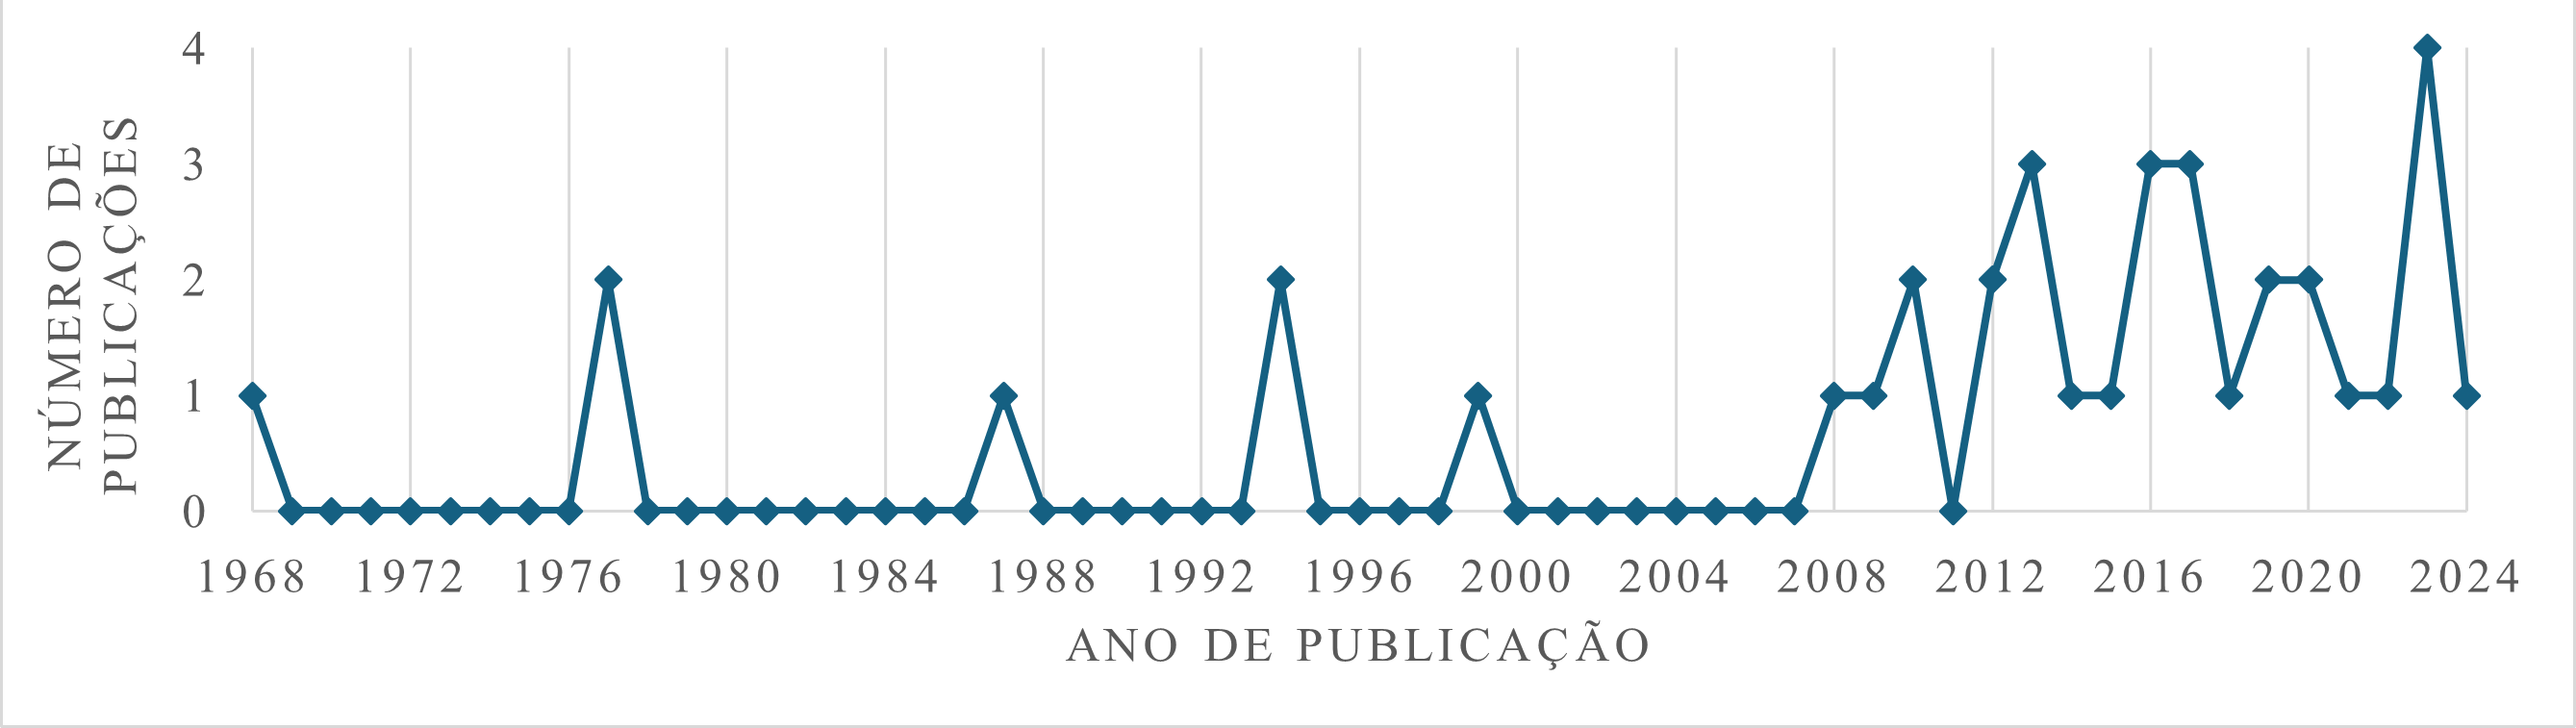
\includegraphics[scale=0.75]{imagens/grafico1.png}
    \fonte{Coleção principal do Web of Science, acesso em maio de 2024.}
    \label{graf:producao_anual}
\end{grafico}

O intervalo encontrado para a produção de artigos sobre FM na WoS foi de 1968 a 2024. Foram encontrados nesse indexador 36 documentos produzidos por 64 autores. A idade média dos textos foi de 13,5 anos, demonstrando que, apesar da frequência com que esses documentos são produzidos ter aumentado a partir de 2008, como é possível observar no Gráfico \ref{graf:producao_anual}, o campo teórico da FM já existe, pelo menos, desde 1968. Os países que mais concentraram publicações foram a Alemanha (11) e os Estados Unidos (10), seguidos pela Holanda (7), Inglaterra (4), México (2), França (1) e Índia (1), demonstrando que o estudo da temática continua concentrado em poucos países. Porém, foi possível observar que há um interesse crescente no estudo da FM.


\section{Fecundidade masculina pelo mundo}\label{tft_tef_mundo}

Cada vez mais há uma percepção de que é relevante compreender os aspectos reprodutivos masculinos, uma vez que a fecundidade masculina possui aspectos específicos, que a distingue da fecundidade feminina. \citeonline{zhang2010male} investigou os diferenciais nas TFTs e das TEFs femininas e masculinas utilizando como fonte principal a publicação \textit{“Demographic Yearbook 2001-Special Topic: Natality Statistics”}\cite{unstatsu25:online2001}. O autor analisou, ao todo, dados de 43 países entre os anos 1990 e 1998, utilizando o intervalo de idade (idade fértil) para as Taxas de Fecundidade Específicas por idade femininas (TEFF) de 15-49 e 15-59 para o cálculo das Taxas de Fecundidade Específicas por idade masculinas (TEFM). A partir de sua pesquisa, \citeonline{zhang2010male} constatou que o coeficiente de variação (CV) para as Taxas de Fecundidade Total Masculinas (TFTM) foi de 0,44, enquanto as Taxas de Fecundidade Total Femininas (TFTF) tiveram o CV de 0,37, indicando uma variação maior nos níveis das TFTMs em relação às TFTFs entre os países analisados. Em seu trabalho, o autor identifica ainda que, em países onde a fecundidade feminina é alta (estabelece TFTF > 2,2), a diferença entre a TFTM e TFTF tende a ser maior, enquanto países com TFTF abaixo desse valor tendem a apresentar taxas comparáveis ou mesmo um nível de TFTF levemente acima da TFTM. Suas conclusões indicam que as TFTMs estão mais espalhadas em relação à média, entre os países analisados, do que as taxas femininas. Ou seja, o número médio de filhos tidos pelas mulheres ao longo de sua vida reprodutiva (nos países analisados) é mais concentrado em torno da média feminina do que o número de filhos tidos por homens em relação a sua média. Adicionalmente, a transição de regimes de alta fecundidade para níveis mais baixos parece influenciar a relação entre fecundidade feminina e  masculina.


 Um segundo trabalho, referência para a área da FM, realiza uma revisão a partir de dados para a idade do pai de 163 países no período por volta de 2011. Nele, \citeonline{schoumaker2019male}, corroborando o que foi encontrado por \citeonline{zhang2010male}, observa que a medida que uma população passa pela transição demográfica, a fecundidade masculina e a feminina se aproximam. O número médio de filhos tidos por mulher variou de 1 a 8 filhos entre os países analisados, enquanto para homens o intervalo encontrado foi bem maior. As TFTMs encontradas pelo autor \footnote{O autor calcula a partir das Taxas de Fecundidade Específicas por idade (TEFs), com 7 grupos etários para mulheres, entre 15 e 49 anos e para homens 13 grupos, entre  15 e 79 anos. } para países da África Subsaariana, foram frequentemente 1,5 a 2 vezes maiores que as TFTFs, combinado com uma população mais jovem e diferenças de idade ao nascimento entre homens e mulheres próximas ou superiores a 10 anos. Enquanto nos países ocidentais, com estruturas etárias mais avançadas, a diferença entre homens e mulheres se mostrou menor, tanto na idade ao nascimento, entre dois e quatro anos, como nas TFTs, com uma razão da TFTM pela TFTF, muitas vezes, inferior a um, ou seja, com a TFTF maior do que a TFTM.

\citeonline{schoumaker2019male} encontra valores mais baixos para a TFTM  nos países europeus, em média entre um e dois filhos, sendo geralmente próximos da TFTF. Os países asiáticos, por outro lado, apresentaram uma variedade maior das TFTMs, com o Japão e a Coreia do Sul apresentando cerca de 1,2 filhos por homem, enquanto outros países do continente apresentam valores bem mais altos, Paquistão (5,1), o Iraque (5,5) e o Afeganistão (6,9). Para os países da América Central e do Sul os valores encontrados foram, no geral, baixos, com o Chile, a Costa Rica e Cuba, variando entre menos de dois filhos, apesar de haver o Haiti como exceção, com TFTM superior a cinco filhos por homem. As TFTMs com valores mais elevados, encontrados pelo autor, se concentraram na África Subsariana, onde, dos 43 países analisados (para essa região), metade possuia uma TFTM superior a 8,5 filhos e um quarto dos países, apresentaram um valor superior a 10 crianças por homem. Seu estudo é eficiente em ilustrar a variabilidade que a fecundidade masculina pode alcançar em diferentes contextos.

Outra contribuição de \citeonline{schoumaker2019male} está em observar que países com alta proporção de mulheres em relações poligínicas\footnote{Estado de um homem que está casado com muitas mulheres. “poliginia”, in Dicionário Priberam da Língua Portuguesa [em linha 2], 2008-2024, https://dicionario.priberam.org/poliginia.} estão relacionados a altos valores para a razão da TFTM pela TFTF. Porém, apesar de ser relevante, a poliginia por si só não se mostrou ser fator explicativo determinante, como o autor chama a atenção, essa diferença costuma estar associada a uma condição necessária à poliginia, a diferença de idade entre os cônjuges numa população com crescimento positivo \apud{pison1986demographic}{schoumaker2019male}.

Nesse sentido, a diferença de idade entre parceiros parece ser um fator importante para os diferenciais na TFT de homens e mulheres. Em trabalho recente, \citeonline{dudel2021male} elencam três possíveis razões para as diferenças encontradas nos valores das taxas de fecundidade masculinas e femininas: 1 - Diferenças de idade entre mães e pais combinado com variação nos tamanhos das coortes; 2 - Diferenças no tamanho das populações feminina e masculina; 3 - Diferenças de gênero no efeito tempo.  

O efeito tempo é uma distorção que pode ocorrer em medidas transversais de fecundidade, como é o caso da TFT. Uma taxa transversal é aquela que mistura eventos de diferentes coortes (ao contrário de taxas que acompanham coortes de maneira longitudinal)\cite{FOZ2021metodos}. Isso faz com que a TFT seja afetada pela experiência de coortes distintas, sendo sensível a mudanças comportamentais temporárias, flutuações de curto prazo que pode ser resultado de um adiamento ou adiantamento momentâneo da fecundidade.

Assim, \citeonline{dudel2021male} propõem que a diferença entre as TFTs masculina e feminina poderia advir de diferenças entre os sexos no  adiamento ou adiantamento da maternidade - paternidade. Segundo os autores, apesar de se observar um padrão geral de pais mais velhos que mães, em diferentes momentos e contextos sociais, alguns fatores, como a revolução de gênero, o aumento do nível educacional entre mulheres, costumam estar associados a um adiamento da maternidade e podem criar condições propícias para a diminuição do intervalo de idade entre parceiros (e.g. pela diminuição da dependência das mulheres em relação à renda do cônjuge).

Embora o adiamento da maternidade seja um tema intensivamente estudado pela demografia no contexto da transição demográfica, relativamente pouca atenção tem sido destinada aos fatores associados ao adiamento da paternidade, com exceção a alguns autores \cite{kyzlinkova2018fatherhood,olah2008sweden,office2009patterns,DenmarkNordfalk} que, no geral, têm mostrado o efeito tempo para os homens, da postergação da idade média ao nascimento, tende a acompanhar o das mulheres, porém muitas vezes se mostrando menos atenuado\footnote{\citeonline{DenmarkNordfalk} encontra um efeito tempo negativo para homens e mulheres dinamarqueses entre 1980-2010, com o efeito para as mulheres, mais evidente do que para os homens}. \citeonline{dudel2021male} chegam a conclusão de que as diferenças no adiamento da idade média ao nascimento entre os sexos e a diferença de idade entre parceiros são fatores relevantes para os diferenciais nas TFTs entre os sexos, apontando para tópicos de pesquisa vitais para o campo da FM. 

No que diz respeito às diferenças no tamanho das populações feminina e masculina, ocorre impacto sobre o denominador no cálculo das TEFs, a população exposta. Por exemplo, se a proporção de homens emigrantes de determinado país é maior que a de mulheres emigrantes, a população masculina diminui, podendo temporariamente aumentar a taxa de fecundidade masculina em relação à feminina. 



\begin{comment}

A combinação de diferentes idades entre mães e pais com a variação nos tamanhos das coortes produz discrepâncias na fecundidade de homens e mulheres porque, se homens e mulheres forem de coortes diferentes e houver variação no tamanho das coortes, o denominador das taxas masculinas e femininas podem diferir. \citeonline{schoumaker2017measuring}, por exemplo, demonstrou em países com altas taxas de crescimento populacional a TFTM cresce mais do que a TFTF, já que os pais costumam vir de coortes menores e de idade mais avançadas do que suas parceiras. 




   -----------------------
     A nossa segunda conclusão principal é que as diferenças de idade entre pais e mães permaneceram constantes ou diminuíram na maioria dos países do nosso estudo, exceto nos países da Europa Oriental e na Alemanha Oriental. Embora esta tendência geral esteja em linha com as expectativas baseadas nas teorias de género, as diferenças que existem actualmente entre os países parecem ser afectadas por mais factores do que apenas diferenças nos níveis de igualdade de género.
    -------------- 


Razão de sexo\footnote{Expressa pelo número de homens para cada grupo de
100 mulheres, na população residente em determinado espaço geográfico, no ano
considerado \cite{rede2002indicadores}.}


encontraram indícios de que as mudanças na razão entre a TFTM e a TFTF são governadas pelas diferenças de idade entre parceiros e em mudanças no comportamento reprodutivo, como adiamento da paternidade e maternidade. Analisaram dados de 17 países de renda alta, no intervalo entre 1968 a 2016 ou 1980 a 2016, para a maioria dos países, e chegaram a algumas conclusões interessantes. Segundo os autores,\textbf{o adiamento da maternidade e da paternidade são fatores...}


From a demographic perspective, such disparities can be driven by three main factors: first, differences in the population sizes of males and females, i.e., in the sex ratio, which can affect both TFR and CFR differences; second, age differences between mothers and fathers in interplay with variation in cohort sizes (affecting the TFR and the CFR); and, third, gender differences in tempo effects, which can impact gender differences in the TFR, but not in the CFR.



---
\textbf{quando os pais são atribuídos à mesma coorte que as mães, e que grandes diferenças de gênero nos níveis de fecundidade são muitas vezes motivadas por diferenças no momento da fecundidade. }


EM WONG 2020- SOBRE SCHOUMAKER 2019:

    The author shows that the TFR of men is almost always higher than that o

women, which he explains by two factors. The first is that men have a higher mortality rate than women, which would lead to fewer men exposed to the risk of parenthood. The second is that men tend to bond and have children with women younger than themselves. If these cohorts of men and women were born in a context of positive population growth, then the cohort of men tends to be smaller than that of women, also decreasing the population at risk of paternity.
\end{comment}

%Taxas Específicas de Fecundidade por idade

Quando falamos do padrão masculino da fecundidade nas faixas etárias, \apudonline{paget1994relational}{zhang2010male}, ao observar países com distintos níveis de TFT nas décadas de 1960-80, identificaram que os homens teriam, em geral, o início de sua vida reprodutiva postergado e uma parada bem posterior em relação às mulheres. Os homens teriam um pico mais tardio e inferior, com as TEFMs permanecendo mais elevadas do que as TEFFs em faixa-etárias mais avançadas. 

\citeonline{zhang2010male} subdivide a análise, com dados para os anos de 1990 a 1998, das TEFs entre países com TFT feminina alta e baixa (TFTM < 2,2 e TFTF < 2,2). O autor encontra que as TEFFs superam as TEFMs nas faixas etárias mais jovens (15–19, 20–24 e 25–29), com o valor médio da TEFFs da faixa etária de 15-19 anos sendo até cinco vezes maior que as TEFMs para esse grupo etário, tanto em países com alta, como com baixa TFT. A faixa de 30 a 34 anos se mostrou um ponto de inflexão na relação da fecundidade masculina com a feminina, sendo observado que nessa faixa as TEFMs começam a superar os níveis das TEFFs, com a razão da TEFM pela TFTF próxima de um. 

{\citeonline{zhang2010male} avança ao descobrir que um fator de mudança na correlação das TEFs feminina e masculina é quando as TFTs se aproximam do nível de reposição demográfica (2,2), quando a TFTM costuma alcançar um patamar inferior a TFTF. As hipóteses que o autor levanta sobre essa questão estão associadas ao denominador no cálculo das taxas de fecundidade, ou seja, mudanças no número de homens na faixa etária. O fato de países com TFT abaixo do nível de reposição serem, geralmente, países de economia desenvolvida pode estar associado a níveis altos de imigração, com o inverso verdadeiro, altas TFTs associadas a menor desenvolvimento e alta emigração. Compreendendo a migração como um movimento feito majoritariamente por homens jovens, isso contribuiria para que o denominador ficasse maior (e uma menor TFTM) em países desenvolvidos e menor em países menos desenvolvidos (TFTM maior). A segunda hipótese, também atrelada aos níveis de desenvolvimento, foca nos diferenciais de mortalidade por sexo. As mulheres costumam desfrutar de uma expectativa mais longa e menores níveis de mortalidade do que homens. O autor conjectura que, em países desenvolvidos, a expectativa de vida masculina pode ser maior e os níveis de mortalidade masculinos menores. Porém, apesar das hipóteses, deixou em aberto o motivo pelo qual a correlação entre TFTM e TFTF se modifica no ponto em que os países alcançam a TFTs no nível de reposição.

\begin{comment}
- diferenças de idade na parturição ---
\cite{dudel2021male}:
----Embora observemos padrões bastante diversos nas diferenças de idade entre países e grupos de países, o mecanismo demográfico subjacente é, em todos os casos, diferenças de gênero no adiamento. Especificamente, em todos os países que estudamos, a idade média ao dar à luz tem aumentado continuamente desde 1990, tanto para homens como para mulheres (ver materiais suplementares para obter detalhes); ou seja, tanto homens como mulheres têm adiado o parto. Em combinação com uma idade média de parto mais elevada para os homens, esta conclusão sugere que as mudanças na diferença de idade parental no momento do parto se devem a diferenças na velocidade com que o adiamento avança: se progredir mais rapidamente entre os homens do que entre as mulheres, a diferença de idade aumenta; mas se, por outro lado, avança mais rapidamente entre as mulheres do que entre os homens, a diferença de idade diminui----

tefs - United Nations Demographic Yearbook 2021




POP ESTÁVEL  (schoumaker)
    Em contraste, os países ocidentais combinam baixas diferenças de idade entre parceiros e estruturas etárias mais avançadas. Ambos os factores estão em jogo nas diferenças entre homens e TFRs femininas, como será demonstrado no caso de populações estáveis. 



IMIGRAÇÃO: (schoumaker)

    O efeito da migração internacional é visível em alguns países onde a razão é muito inferior ao esperado devido à diferença de idade (por exemplo, no Bahrein e no Qatar, com grande imigração masculina), ou superior ao esperado em países com grande emigração masculina, como no Nepal com o DHS. Em contraste, as estimativas que corrigem a migração internacional (seja no Nepal ou no Qatar) estão mais em linha com outras estimativas.

    (ZHANG)
When the cumulative pattern of fertility is considered, male total fertility rates (TFRs) are found to be different from those of females. It is shown that male TFRs were first higher than female TFRs in most Western industrialized countries before the 1960s. Such male and female fertility differentials are likely to be resulted from the relative shortage of men caused by two world wars. Since the 1960s, males in most industrialized countries have recovered from war time losses. Coupled with an increasing emigration that has been replaced by immigration which is largely dominated by men, male TFRs turned to be higher than female TFRs afterwards (Coleman, 2000). In addition to male and female fertility differentials in rates, demographers have also indicated that the progeny size distribution and childlessness patterns of men and women differentiate male fertility from female fertility.

\end{comment}


\begin{comment}
    A nossa segunda conclusão principal é que as diferenças de idade entre pais e mães permaneceram constantes ou diminuíram na maioria dos países do nosso estudo, exceto nos países da Europa Oriental e na Alemanha Oriental. Embora esta tendência geral esteja em linha com as expectativas baseadas nas teorias de gênero, as diferenças que existem atualmente entre os países parecem ser afetadas por mais factores do que apenas diferenças nos níveis de igualdade de gênero. Embora as nossas descobertas indiquem que a fecundidade masculina tem sido geralmente inferior à fecundidade feminina nos últimos anos, esta tendência não parece manter-se a nível mundial. 

    Schoumaker (2017, 2019) mostrou que em contextos em que a poliginia é praticada e as populações estão a crescer rapidamente, os níveis de fecundidade masculina podem por vezes ser duas vezes superiores aos níveis de fecundidade feminina. Seus resultados sugerem que esse padrão é impulsionado, em grande parte, pelas diferenças de idade entre os casais. 
    
    Esta conclusão está em linha com os resultados da nossa análise contrafactual, que indicam que os casos extremos tendem a desaparecer quando os pais são atribuídos à mesma coorte que as mães, e que grandes diferenças de gênero nos níveis de fecundidade são muitas vezes motivadas por diferenças no momento da fecundidade. . No outro extremo, o razão TFT mais baixo relatado na literatura é para Inglaterra e País de Gales em 1973, em torno de 0,89 (Schoen 1985). O valor que encontramos para a Alemanha Oriental, 0,84, está abaixo deste nível e pode indicar que os homens da Alemanha Oriental têm experimentado o que Schoen (1985) chamou de “aperto de natalidade”: ou seja, na Alemanha Oriental, o número desigual de homens e mulheres na faixa etária reprodutiva está tendo impacto na fecundidade dos homens. Geralmente, a variação nas razões TFR que observamos entre países e ao longo do tempo não é negligenciável. Os grupos de países com semelhanças culturais e/ou políticas parecem ter padrões de tendências mais semelhantes. Esta descoberta requer uma investigação mais aprofundada.




---- 
dudle 2016: 

as diferenças de idade dos pais aumentaram para as mães mais jovens e diminuíram para as mães mais velhas; e a heterogeneidade entre as faixas etárias aumentou. As inclinações para os homens apresentam menos variação do que as inclinações para as mulheres. 

na perspectiva dos pais, as diferenças de idade entre os pais têm geralmente diminuído, mas também tem havido um padrão bastante estável de pais mais velhos que tendem a ter filhos com mães muito mais jovens.

“observations that men generally prefer younger partners as they become older, while women’s age preferences for their partners are more heterogeneous (Skopek, Schmitz, and Blossfeld 2011).” ([Dudel et al., 2020, p. 13](zotero://select/library/items/XGG8CKCJ)) ([pdf](zotero://open-pdf/library/items/54XEELWP?page=14\&annotation=LPQ2UYNK))

a mudança nas diferenças de idade dos pais ao longo do tempo foi influenciada pelo género. Para as mulheres, esta mudança levou a uma maior heterogeneidade entre idades, de tal forma que as diferenças de idade dos pais entre mães mais jovens e mais velhas diferem mais hoje do que no passado. Entre os pais, por outro lado, as diferenças de idade parentais diminuíram, independentemente da idade em que tiveram um (outro) filho. Estas observações estão em linha com as conclusões existentes de que as alterações na fecundidade por estatuto social ou por idade que ocorreram nas últimas décadas foram muito maiores para as mulheres do que para os homens (ver Jalovaara et al. 2018). Uma possível explicação para isto é que o estatuto socioeconômico das mulheres tem vindo a mudar mais rapidamente. No entanto, embora seja claro que os padrões de disparidades de idade dos pais são de gênero, os resultados das nossas análises de regressão indicam que a diminuição das diferenças de idade dos pais que são atribuíveis ao atraso na parentalidade apresenta regularidades notáveis entre países ao longo do tempo.

indicam que, para as mulheres, o parto mais tardio está associado a uma menor diferença de idade parental; e, portanto, com uma relação de poder mais equilibrada. Nas últimas décadas, detectamos que as mães mais jovens têm filhos com parceiros cada vez mais velhos, o que sugere que é cada vez mais provável que estejam numa união com relações de poder desiguais. Para os pais, o parto mais tardio está associado a uma maior diferença de idade parental, o que implica que estes tenham maior poder na relação. No entanto, este efeito tem diminuído ao longo do tempo à medida que o adiamento da fecundidade aumentou entre homens e mulheres.” ([Dudel et al., 2020, p. 13]


\end{comment}

\begin{comment}

FATORES SOCIOLÓGICOS, ESTUDOS DE GÊNERO E PREFERENCIAS REPRODUTIVAS ENTRE HOMENS E MULHERES: 
\begin{itemize}
    \item Challenging Demography: Contributions from
Feminist Theory (Nancy E. Riley)
    \item Masculinity: An Overlooked Cultural Influence on Fertility
Rachael S. Pierotti, University of Michigan
\end{itemize}


SOCIOLOGICO (zhang) 
    Beyond investigating fertility determinants, examining other dimensions of fertility needs involving males as well. For example, understanding the timing of parenthood demands exploring closely the meaning of fatherhood and motherhood in various cultural institutions and how the meaning changes over the life course for men as compared to for women. Looking into the link between the construction and deconstruction of a childbearing and childrearing union (such as cohabitation and marriage) also requires knowing more about men’s commitment in these unions. The women’s health movement has also stressed the need for men to be aware of their responsibilities in family planning and reproductive health. In sum, it is imperative to bringing men into fertility and fertility-related research. Male fertility should be considered as an important component of fertility studies.


https://citeseerx.ist.psu.edu/document?repid=rep1&type=pdf&doi=db7234060968eb15b6239c3661d5dcac5159c3a5 
    Este artigo demonstra que a educação influencia o comportamento reprodutivo dos homens de múltiplas maneiras. Centrando-nos particularmente na falta de filhos e na fecundidade multiparceira, os elementos-chave nas nossas análises são factores relacionados com a capacidade de um homem para uma parentalidade económica e prática, reflectida, por exemplo, na sua capacidade parental. através das perspectivas de rendimento, da segurança no emprego, da flexibilidade laboral e da composição de género do emprego.

\citeonline{goldscheider1996fertility}





- estudos atuais(relevancia atual):  \cite{keilman2014measures}, \cite{gerber2014two}


\section{referencias do Zhang -- antigas:}

\begin{itemize}
  
    \item Os efeitos da idade na fecundidade masculina e feminina também são muito diferentes. As mulheres atingem seu pico de fecundidade entre 25 e 35 anos, após o qual a fecundidade começa a declinar até a menopausa. Já os homens continuam a ter capacidade reprodutiva até a morte, embora de forma gradual (Wood, 1994). 
    \item Quando o padrão cumulativo de fecundidade é considerado, as taxas de fecundidade total masculina (TFR) são encontradas como diferentes das femininas. Observa-se que as TFR masculinas eram maiores que as femininas na maioria dos países industrializados ocidentais antes dos anos 1960.
        \begin{itemize}
            {\item Essas diferenças de fecundidade entre homens e mulheres provavelmente resultaram da relativa escassez de homens causada pelas duas guerras mundiais. Desde os anos 1960, os homens na maioria dos países industrializados recuperaram-se das perdas da guerra. Aliado ao aumento da emigração substituída pela imigração predominantemente masculina, as TFR masculinas passaram a ser maiores que as femininas (Coleman, 2000)}
       \end{itemize}
    \item Além das diferenças nas taxas de fecundidade entre homens e mulheres, demógrafos também indicaram que a distribuição do tamanho da prole e os padrões de ausência de filhos diferenciam a fecundidade masculina da feminina. Algumas pesquisas mostram que, em geral, os homens têm menos filhos que as mulheres. 
    Consequentemente, há percentagens mais altas de homens sem filhos em comparação com as mulheres (Coleman, 2000). Todos esses fatos sugerem que a fecundidade humana não pode ser totalmente representada pela fecundidade feminina. Usar as taxas de fecundidade feminina para representar as masculinas pode ser problemático, especialmente em sociedades onde as taxas de divórcio, novo casamento e migração são bastante altas. Pesquisadores sugerem que mesmo aplicar as taxas de fecundidade feminina marital para representar a fecundidade humana como uma solução alternativa é inadequado, pois as taxas de nascimentos não maritais em algumas sociedades são comparativamente altas e os homens têm mais probabilidade de se casar novamente após o divórcio do que as mulheres, o que torna a fecundidade masculina e feminina não comparável (Greene \& Biddlecom, 2000; Juby \& Bourdais, 1998; Magnani, Bertrand, Makani, \& McDonald, 1995).

    \item Além de investigar os determinantes da fecundidade, examinar outras dimensões da fecundidade também exige envolver os homens. Por exemplo, entender o momento da paternidade exige explorar de perto o significado da paternidade e maternidade em várias instituições culturais e como o significado muda ao longo da vida para homens em comparação com mulheres. Analisar a ligação entre a construção e desconstrução de uma união de criação de filhos (como coabitação e casamento) também requer saber mais sobre o compromisso dos homens nessas uniões. O movimento pela saúde da mulher também destacou a necessidade de os homens estarem cientes de suas responsabilidades no planejamento familiar e na saúde reprodutiva. Em suma, é imperativo incluir os homens nas pesquisas de fecundidade e relacionadas à fecundidade. A fecundidade masculina deve ser considerada um componente importante dos estudos de fecundidade.
\end{itemize}






-----------
\end{comment}
\section{Principais bases e métodos}\label{bases_e_metodos-ref}


A TFT e as TEFs são geralmente calculadas para mulheres, porém, como defendemos aqui, ambas podem e devem ser calculadas também para homens. As TEFs por idade (${}_n{f}_x$, onde $x$ é o limite inferior da faixa de idade e $n$ o tamanho do intervalo, geralmente intervalos quinquenais de idade) relacionam-se ao número de nascimentos ocorridos entre homens de uma determinada idade ou grupo etário com o tempo total de exposição dos mesmos ao risco de terem filhos naquele mesmo período \cite{FOZ2021metodos}. Definida por:

\begin{equation}\label{tefmEqu}
{}_n{f}_x = 1000 \cdot \frac{\text{\footnotesize \textit{Número de nascimentos ocorridos aos homens com idades entre} } x \text{ \footnotesize e } x + n \text{ \footnotesize \textit{no período}}}{\text{\footnotesize \textit{População média de homens com idades entre} } x \text{ \footnotesize e } x + n \text{ \footnotesize \textit{no período}}} \\
\end{equation}

Já a TFTM quantifica o número médio de filhos nascidos vivos que um homem teria ao longo dos seus anos reprodutivos, se fosse exposto às TEFs masculinas de um determinado ano. Como vimos anteriormente\footnote{Seção \ref{tft_tef_mundo}}, a TFT pode ser afetada quando ocorre um adiamento ou adiantamento da paternidade-maternidade. Porém, é um dos indicadores mais relevantes para caracterizar o nível da fecundidade da população de determinado território ou grupo social. É obtido somando as TEFs (${}_n{f}_x$) e multiplicando pela amplitude do grupo etário $n$, onde $\alpha$ e $\beta$ indicam o início e o fim do intervalo reprodutivo masculino:

\begin{equation} \label{tftEqu}
TFT = n \sum_{x=\alpha}^{\beta} {}_n{f}_x
\end{equation}


Não há consenso sobre o intervalo utilizado para o período reprodutivo masculino, sendo utilizados diferentes intervalos entre os autores (15-59, 15-79, 17–59, 15-50, 15-59, 20-59\footnote{\citeonline{zhang2010male,schoumaker2019male,dudel2016estimating, kyzlinkova2018fatherhood, unstatsu2022Nota} e \citeonline{office2009patterns}, respectivamente. Alguns autores adotam intervalos diferentes conforme limitações da base de dados.}). A maioria dos autores agrupa os nascimentos observados fora do limite superior e inferior nas coortes limites. Por exemplo, considerando nascimentos com idade masculina observada menor de 14 anos, parte do grupo etário 15-19 anos. Nascimentos abaixo de 15 anos e acima de 60 costumam ser apontados como eventos rarefeitos.  
  

Conforme vimos a partir de \citeonline{zhang2010male}, os estudos de fecundidade masculina têm como uma de suas principais barreiras, a qualidade dos registros para idade do pai ao nascimento, informação necessária para se obter o numerador do cálculo das TEFMs (equação \ref{tefmEqu}). Os dados de fecundidade masculina estão disponíveis em muitos países ocidentais através do registo civil e sistemas de estatísticas vitais (CRVS). O \textit{“United Nations Demographic Yearbook”} compila o número de nascidos vivos por idade do pai e calcula as TEFMs através de registros civis e é uma das principais bases que tem sido utilizadas para os estudos de fecundidade masculina pelo mundo. A publicação é baseada em dados coletados das autoridades nacionais de estatística de diversos países, desde 1948. Ela é considerada uma das bases mais completadas que contém informação sobre fecundidade masculina, apresentado dados nas edições de 1949–1950, 1954, 1959, 1965, 1969, 1975, 1981, 1986, 1999 e 2007-2022 \cite{unstatsu25:online}. Porém, a base possui limitação quanto a sua abrangência. Sendo composta majoritariamente por nações onde os CRVS são mais avançados \cite{zhang2010male} e atingem maior completude, ou seja, com baixa proporção de dados faltantes. Essa foi a principal fonte de informação utilizada nas análises de \citeonline{zhang2010male} e \citeonline{paget1994relational}. 

Visando ampliar a análise da fecundidade masculina para países não abarcados pelo \textit{“United Nations Demographic Yearbook”}, \citeonline{schoumaker2017measuring} elabora e compara três métodos para estimar as TEFMs utilizando as bases do \textit{“Demographic and Health Surveys (DHS)”}\footnote{Pesquisa de saúde realizada a mais de 30 anos em cerca de 90 países. Dentre as informações coletadas (sobre mortalidade infantil, fecundidade, planejamento familiar, saúde materna, imunização infantil, níveis de desnutrição, prevalência do HIV e malária) estão aspectos relacionados a fecundidade e reprodução masculina. Fonte: https://www.usaid.gov/global-health/demographic-and-health-surveys-program.}. As pesquisas do programa DHS se estruturam por três questionários, aplicados aos moradores, à mulher selecionada (entre 15-49 anos) e ao homem selecionado (geralmente entre 15-59 anos). O autor utiliza os dados disponíveis para encontrar o número de nascimentos ocorridos aos homens nas faixas idades. Os três métodos utilizados foram: método dos filhos próprios \textit{(own-children method)}, o método da data do último nascimento \textit{(the date-of-last-birth method)} e o método cruzado \textit{(the crisscross method)}.



O método dos filhos próprios (MPF), utilizado habitualmente para calcular a fecundidade feminina, foi adaptado pelo autor para o caso dos homens mediante basicamente cinco passos: parear a criança sobrevivente com o respectivo pai, classificar os filhos por idade e por idade do pai em dado ano, redistribuir as crianças não correspondidas por idade do pai, reverter a sobrevivência das crianças para estimar o número de nascimentos por ano e idade do pai nos anos anteriores ao levantamento, e  reverter a sobrevivência da população masculina nos anos anteriores à pesquisa para estimar o denominador das TEFMs \cite{schoumaker2017measuring}. 
Formalmente, a TEFM no período entre $x$ e $x+1$ anos antes do momento da pesquisa, para homens que naquele momento tinham entre $y-x-1$ e $y-x$ anos deve ter sido: 

\begin{equation}
    TEFM_{y-x}(t-x-\text{\footnotesize1/2})=P_{x,y}\frac{\ell_{0}}{\ell_{x+\frac{1}{2}}} / P_{y}\frac{\ell_{y-x}}{\ell_{y+\frac{1}{2}}}
\end{equation}

No numerador temos ($P_{x,y}$) filhos atualmente vivos (sobreviventes dos que nasceram num momento passado), crianças de $x$ anos completos de idade cujos pais têm $y$ anos, multiplicado pela razão de sobrevivência da criança no intervalo ($P_{x,y} \ell_{0} / \ell_{x+\frac{1}{2}}$). O denominador é composto pelos pais atuais, sobreviventes dos que haviam na época, através de $P_{y}$ $\ell_{y-x} / \ell_{y+\frac{1}{2}}$ \cite{FOZ2021metodos}.  

Para o primeiro passo, parear as crianças sobreviventes aos seus respectivos pais (para obter idade dos pais ao nascimento), \citeonline{schoumaker2017measuring} utiliza informações inclusas nos próprios dados da DHS, disponíveis para quando ambos residem na mesma casa. Para o caso no qual o pai vive em casa diferente, o autor estimou as idades dos pais sobreviventes utilizando por registro doador (Hot-Deck) \apud{allison2001missing}{schoumaker2017measuring}, retirando crianças sobreviventes que relataram que seus pais não eram mais vivos. 
A idade do pai para os filhos cujo pai está vivo foi então imputada para cada filho não pareado, um filho com as mesmas características (idade e idade da mãe) foi selecionado aleatoriamente entre os filhos pareados\footnote{O autor realizou a imputação aleatória 10 vezes e calculou 10 séries das TEFMs, considerando, ao final, a média das 10 séries de TEFMs}.
A idade do pai do filho selecionado foi então atribuída ao pai do filho sem correspondência.
O autor afirma que se seguisse a abordagem padrão para o MFP (normalmente aplicado para o cálculo das TEFF), iria supor a mesma distribuição de idade dos pais de filhos compatíveis e de filhos não correspondidos de idade $x$, usar a idade da mãe no processo de imputação levou a uma idade ao nascimento mais baixa (um ano em média) para pais de filhos não correspondidos em comparação com pais de filhos pareados. Em seu processo de estimação, o autor encontrou que outras informações poderiam ser consideradas no processo de imputação, como o tipo de local de residência, porém demonstraram ter um impacto limitado nos resultados. 

Em seguida, para encontrar um pai (de idade imputada) para filhos não pareados, um homem com a mesma idade que a idade imputada do pai  foi selecionado aleatoriamente entre os homens no conjunto de dados do agregado familiar, independentemente do homem já ser pai ou não. Os últimos passos foram, estimar o número de nascimentos em $x$ anos antes da pesquisa (através do inverso da probabilidade de sobrevivência dos filhos com idade completa $x$) para, por fim, calcular as TEFMs, os nascimentos durante os cinco anos anteriores à pesquisa são somados por faixa etária dos pais ao nascimento, e a exposição é obtida somando o tempo que cada homem passou em cada faixa etária nos últimos cinco anos.

O segundo método proposto por \citeonline{schoumaker2017measuring} foi o da data do último nascimento. Nele, é pressuposto que as TEFMs são constantes para o grupo etário $j$ em dado período. As taxas de fecundidade no grupo etário $j$ ($\lambda_{j}$) são calculadas como a razão entre o número de nascimentos visíveis (últimos nascimentos) no grupo de idade $j$ e a exposição dos homens nessa faixa etária naquele período, medido como a soma da duração (para cada homem) passada na faixa etária entre a data do inquérito e a data do último nascimento, ou a data do início do período, se nenhum nascimento ocorreu durante o período (faixa do grupo etário, por exemplo, cinco anos). No método não é possível captar caso tenha ocorrido mais de um nascimento para o pai durante o período, o que gera subestimação da fecundidade. Porém, uma vantagem dessa escolha, segundo o autor, é de que seria possível  analisar as TEFMs entre diferentes grupos, com seus marcadores sociais ou características como tipo de relação monogâmica-poligínica, isso porque o número de nascimentos visíveis por grupo etário 
 é uma informação obtida diretamente do questionário dos homens selecionados.  


\begin{equation}
   TEFM (\lambda_{j}) = \frac{\text{\footnotesize \textit{número de nascimentos visíveis por grupo etário} }j}{\text{\footnotesize \textit{exposição visível no grupo etário}}j}
\end{equation}


Na terceira e última abordagem exposta por \citeonline{schoumaker2017measuring}, o método cruzado, é feito uma comparação entre os dados das crianças nascidas vivas em duas edições da DHS. TEFMs ($\lambda$) entre duas idades $x$ e $x+n$ sobre um período ($t$) são estimadas pela equação “crisscross”\footnote{Para maiores detalhes ver o trabalho \textit{“The crisscross method to evaluate data quality in fertility surveys”}\cite{schoumaker2014crisscross}, onde o autor detalha melhor seu método.}. Utiliza-se o número médio de crianças já nascidas por idade exata, estimado suavizando o número de crianças já nascidas por idade completa. As vantagens desse método seria que, por se basear no número de crianças já nascidas, não seria afetado por imprecisões nas datas de nascimento ou idades das crianças. No entanto, seria impactado por omissões diferenciais de nascimentos nos inquéritos e diferenças na composição da amostra entre edições da DHS (e.g. se homens com fecundidade elevada forem sub-representados).

A principal contribuição do trabalho de \citeonline{schoumaker2017measuring} é possibilitar a estimação da fecundidade masculina em países onde os registros administrativos não são totalmente consolidados. O Brasil tem bases da DHS para os anos de 1986, 1991 e 1996, disponíveis no site do programa DHS \footnote{Fonte: \href{https://dhsprogram.com/Countries/Country-Main.cfm?ctry_id=49\&c=Brazil}{Programa DHS - Brasil.}}, porém, em 1991, foi realizada uma pesquisa de Demografia e Saúde da Mulher e da Criança com abrangência somente para o Nordeste\footnote{\href{https://dhsprogram.com/publications/publication-FR5-DHS-Final-Reports.cfm}{Relatório Final - Pesquisa sobre Saúde Familiar no Nordeste Brasil 1991}}. Em 2006, foi realizada a Pesquisa Nacional de Demografia e Saúde da Criança e da Mulher (PNDS) nos moldes da 5ª fase do projeto DHS e está previsto para 2025 o resultado da PNDS de 2023, baseado na 8ª rodada do programa. A PNDS 2023 será a primeira a fornecer histórico de filhos biológicos nascidos vivos, para homens entrevistados de 15 a 59 anos, informação que poderá ser utilizada para cálculo da fecundidade masculina. As edições de 1991 (com abrangência para o Nordeste) e de 1996 tiveram questionários aplicados ao 'marido' e ao homem selecionado.  

\citeonline{wong2020LatinA} estimam as TEFMs e a TFTM utilizando métodos indiretos a partir de microdados disponíveis na plataforma do \textit{“Integrated Public Use Microdata Series (IPUMS), International”}, dos censos do Brasil, Argentina, Chile, Colômbia, Equador, México, Paraguai, Uruguai e Venezuela desde 1970. O método utiliza informações sobre a composição familiar e assume que o cônjuge ou companheiro da mulher que teve um filho nascido vivo nos 12 meses anteriores ao censo é o pai da criança. A partir do quesito que pergunta às mulheres sobre nascidos vivos nos últimos 12 meses ou pela idade do filho mais novo, calcula-se a fecundidade de período para os homens. Para estimar as idades dos pais ausentes (mulher solteira), os autores utilizaram a imputação condicional à idade da mãe, na qual a idade do pai-cônjuge ausente é a média de idade dos pai-cônjuges observados $b$ das mulheres em idade $a$, em cada país e ano \cite{wong2020LatinA}. 

\begin{equation}
    \hat{b} = E[b|A=a]
\end{equation}

As TEFMs foram obtidas pela divisão do número de nascimentos, pelo número de homens, no grupo etário. Os autores, buscaram corrigir possíveis fontes de erro (erro no registro do período de referência, subestimação do número de crianças na casa) a partir de um fator de correção, comparando a TFT feminina calculada pelo método indireto do artigo com a estimada pelo \textit{UN World Prospects\footnote{\href{https://population.un.org/wpp2019/}{World Population Prospects 2019.}}} (mantendo o padrão etário da população de cada país no momento do censo).     

Houve alguns autores que tentaram contornar o problema da qualidade dos registros administrativos e estimar a fecundidade masculina em países onde havia uma proporção considerável de dados faltantes. No Brasil, \apudonline{Wong1986}{wong2022fecundidade} usaram dados administrativos para calcular a fecundidade
masculina em São Paulo(SP) em 1983. Reportaram que, à época, cerca de 10\% dos registros de nascimento estavam com a idade do pai como “ignorada”. Infelizmente não consegui acesso ao artigo original das autoras para verificar se foram utilizadas técnicas de imputação. 

\citeonline{falcao_fecundidade_2013} utilizou microdados do Sistema de Informação sobre Nascidos Vivos (SINASC) e informações do Sistema Estadual de Análise de Dados - SEADE (para o denominador, distribuição da população por sexo e idade) para estimar a TFTM e as TEFMs para alguns municípios de SP. O critério de seleção dos municípios no artigo foi aqueles que possuíam um registro superior a 1.500 nascimentos no ano, e aqueles nos quais os registros com idade do pai não declarada fossem inferior a 8,0\%. Apenas 14 municípios paulistas do ano selecionado (2013) cumpriram os dois critérios. O autor limita, em sua análise, o período reprodutivo masculino de 15 aos 59 anos, após observar que os registros com pais acima de 60 anos não eram suficientemente robustos para alterar a TFTM. Em sua análise, \citeonline{falcao_fecundidade_2013} utiliza apenas os registros que possuem idade do pai observada, deletando os registros com idade do pai ausente.    

\citeonline{dudel2019estimating} utilizam registros administrativos da
Suécia (1968-2014), EUA (1969-2015), Espanha (1975-2014) e Estônia (1989-2013), onde a idade do pai é faltante em cerca de 1\%, para a maioria dos anos na Suécia, mas chegou a 17\% no início da década de 1990 nos EUA. Os autores problematizam a abordagem utilizada por alguns autores para lidar com o problema dos dados faltantes para a idade do pai, adotada também pelo “United Nations Demographic Yearbook”\cite{unstatsu2022Nota}. Normalmente os nascimentos de pais de idade desconhecida são distribuídos proporcionalmente pelas faixas etárias, de acordo com a distribuição dos nascimentos por idade do pai antes do cálculo das taxas. Dessa forma, é pressuposto que a idade do pai é ausente por motivos totalmente aleatórios e que a distribuição das idades não registradas é a mesma das observadas. \citeonline{dudel2019estimating} discordam dessa abordagem e comprovam, através da simulação de 71.550 cenários, que a imputação das idades paternas faltantes condicionada pela idade da mãe observada tem um melhor desempenho na grande maioria das simulações.  

Em seu trabalho, \citeonline{dudel2019estimating} distribuem as idades do pai não observadas de duas maneiras, condicional e não condicional à idade da mãe (assumida como sempre observada), e testam, ao final, qual das duas abordagens apresenta melhor desempenho, estimando as TEFMs para os países em determinado ano. Onde $B(x,t)$ denota os nascimentos de homens em idade $x$ no tempo $t$, $N(x,t)$ referencia a população exposta de homens em idade $x$. A TEFM calculada, como anteriormente, pelos nascimentos sobre a população exposta é dado por: $f(x,t)=B(x,t)/N(x,t)$, retirando-se o índice $t$ para simplificar as fórmulas. $B(\ast)$ representa o número de nascimentos com idade do pai desconhecida e $B^*(x)$ os nascimentos com idade do pai observada. 


Na abordagem incondicional, $B(\ast)$ (idades não observadas) são distribuídas conforme as idades observadas $B^*(x)$ e $P^*(x)$ é a proporção de pais em idade $x$ calculada ignorando valores ausentes. O cálculo da TEFM é expresso da seguinte forma: 

\begin{equation}
    f(x)=\frac{B^*(x)+B(\ast)P^*(x)}{N(x)}
\end{equation}

Para a abordagem condicional, considera-se $B^*(x,y)$ o número de nascimentos de pais em idade $x$ e mães em idade $y$. $P^*(x|y)$ é a distribuição da idade paterna condicional à idade da mãe, a partir dos valores observados para idade do pai, calculados: $B^*(x,y)/ \sum_{i=\alpha}^{\beta}B^*(i,y)$, onde $\alpha$ e $\beta$ representam a primeira e a última idade reprodutiva dos homens; $B(\ast,y)$ representa o número de nascimentos para os quais a idade materna é conhecida e igual a $y$ e a idade paterna é desconhecida. Assim, pela abordagem condicional, a TEFM é calculada (onde $\gamma$ e $\delta$ denotam as idades mais nova e mais velha das mulheres): 

\begin{equation}
    f(x)=\frac{B^*(x)+\sum_{j= \gamma}^{\delta}  B(\ast, j)P^*(x|j)}{N(x)}
\end{equation}





\begin{comment}

(fazer uma tabela mostrando os métodos já propostos e as bases utilizadas, seus pós e contra --\textit{shoumaker})


problema do método de estimar pelos filhos que coabitam residencia com os pais: 
mudanças no padrão de casamento, multiparentalidade--- >

https://journals.library.ualberta.ca/csp/index.php/csp/article/view/15837/12642
.....

FECHAR FALANDO SOBRE O PORQUE ESCOLHER A METODOLOGIA QUE ESCOLHI PARA TRATAR O DADO... 

\end{comment}





\section{Fecundidade masculina no contexto brasileiro}

A fecundidade, em comparação com mortalidade, é um componente da dinâmica demográfica fortemente afetado pelo contexto social. Numa perspectiva de estrutura e agência, as circunstâncias históricas e o território compõem o quadro de ações possíveis dos sujeitos, dos constrangimentos estruturais que guiarão a trajetória de vida de um indivíduo em determinada sociedade. Nesse sentido, a fecundidade masculina e as preferências reprodutivas podem apresentar determinantes específicos guiados pelos significados da construção da paternidade no Brasil e na América Latina.

\citeonline{giffin1999homens} analisando uma série de estudos (majoritariamente qualitativos) das décadas de 1980 e 1990, mostram que a fala masculina sobre sexualidade e afeto e da relação de homem-mulher é condicionada por um padrão histórico que ressalta a hierarquia dos gêneros e a desvalorização desses assuntos, vistos como femininos. De fato, o papel mais próximo que os homens parecem ocupar nas análises sobre aspectos reprodutivos parece ser sobre a sua influência enquanto cônjuge na utilização de contraceptivos de suas parceiras \cite{carvalho2001participaccao}. Pensar sobre os processos reprodutivos masculinos e seu impacto nas dinâmicas demográficas e sociais é essencial para identificar fatores que tem impactado na redução da fecundidade no país, principalmente no contexto das mudanças sociodemográficas recentes, tais como taxas mais elevadas de divórcio, aumento da participação da mulher no mercado de trabalho, transformações na organização do domicílio, urbanização, que passaram a demandar maior envolvimento dos homens na criação dos filhos. 

Em consistente decrescimento desde a década de 1960, a TFT brasileira atingiu, já no censo de 2010, patamar abaixo daquele do necessário à reposição populacional (2,1 filhos nascidos vivos por mulher). Segundo projeção do \textit{“World Population Prospects 2022”}\cite{desa2022united}, o total populacional brasileiro deve começar a declinar já próximo do início da década de 2050. Tais mudanças no cenário colocam em foco o estudo da fecundidade na demografia brasileira, de maneira geral. A transição da fecundidade brasileira é um fenômeno que está ocorrendo rapidamente, passando de um país com cerca 6,1 filhos por mulher na década de 1950 para o cenário atual. 

A fecundidade, também no Brasil, é abordada, quase que de maneira universal, como um fenômeno feminino, com seus determinantes e seus diferenciais segundo as variáveis demográficas (cor-raça, região, nível educacional, etc.) sendo, ainda que não exaustivamente, bem documentados\footnote{Para citar alguns exemplos: \cite{gonccalves2019transiccao,berquo2014notas,wong1984niveis,wong1983fecundidade}}. A fecundidade masculina, por outro lado, tem se mantido como uma área em que poucos pesquisadores ousaram adentrar. Alguns trabalhos \cite{gerber2014two, Caswell2022-zu}, porém, têm demonstrado a importância de considerar também a fecundidade masculina nas principais análises demográficas.

O trabalho de \apudonline{Wong1986}{wong2022fecundidade} foi pioneiro no Brasil nos estudos da FM. As autoras realizaram algumas análises utilizando dados administrativos\footnote{Como veremos no capítulo \ref{Sinasc&DNV}, à época o Sinasc ainda não havia sido criado.} do estado de São Paulo no ano de 1983. Seus resultados demonstraram (como visto na seção anterior) que, no ano analisado, em cerca de 10\% dos registros de nascimento de SP a idade do pai aparecia como “ignorada”. As autoras também observaram que a fecundidade masculina para o estado atingiu seu nível máximo entre os homens que tinham entre 20 e 30 anos e que, entre as mulheres, esse nível dava-se cerca de 5 anos antes, corroborando resultados encontrados na literatura que mostraram que o pico da fecundidade masculina é posterior ao feminino.

No que foi uma das primeiras pesquisas a investigar aspectos reprodutivos masculinos nacionalmente, a PNDS 1996 entrevistou homens entre 15 e 59 anos. Na época, a pesquisa encontrou que 87\% dos homens unidos declararam ter pelo menos um filho. 56\% dos homens relataram nunca terem tido filhos, 27\% ter um ou dois filhos e 17\% pelo menos três\apud{badiani1998homens}{falcao_fecundidade_2013}. A diferença na idade mediana ao casar entre homens e mulheres era em torno de três anos, enquanto a idade mediana na primeira relação para homens era de 16,7 anos mostrando que eles começavam a vida sexual aproximadamente 2,8 anos mais cedo do que as mulheres, de maneira oposta ao que acontece com o casamento, em que o homem casaria três anos mais tarde\cite[Tabela 5.7]{bemfam_brasil_1997}.

Mais recentemente, \citeonline{wong2020LatinA} traçaram um panorama da TFT masculina entre os anos de 1970 e 2010, mediante métodos indiretos aplicados a dados censitários disponíveis na plataforma do \textit{IPUMS International}\footnote{Citado na seção anterior (\ref{bases_e_metodos-ref})}. Os autores encontraram que, no Brasil,
o diferencial\footnote{(TFTM - TFTF)} entre a TFTM e a TFTF passou de, aproximadamente, 1,3 em 1970, para 0,2 filhos em 2010. A TFTM caiu em média 1,06 a cada década, tendo o valor inicial, em 1970, de 6,2 filhos por homem e valor final de 2,0, em 2010. Enquanto isso, a TFTF encontrada pelo método dos autores foi de 5,0 no mesmo período inicial e 1,8 em 2010, reduzindo 0,79 a cada 10 anos. Calculando a idade média da fecundidade de homens e mulheres, encontraram que, na década de 70, o valor para a população masculina era de 36,2 e para mulheres 29,8 anos, já no final do período, em 2010, os valores foram de 32,5 e 26,6, respectivamente. A diferença entre sexos para a idade média da fecundidade apresentou pouca variação, sendo de 6,4 em 1970 e 6,0, em 2010.

A análise realizada no trabalho de \citeonline{wong2020LatinA} segue o padrão observado em outros países, onde a diferença entre as TFTs masculina e feminina diminuem a medida que o país passa pela transição demográfica. A TFT masculina decresceu em ritmo mais acelerado que a feminina, com valores muito próximos ao final do período analisado. Apesar disso, a diferença da idade média da fecundidade permaneceu alta. Os autores argumentam que a queda (para ambos os sexos) do indicador pode ser parcialmente explicado devido ao crescimento da fecundidade adolescente na América Latina durante o intervalo estudado. No Brasil, a tendência alcançou o nível mais baixo para homens e mulheres na década de 2000, com uma leve subida em 2010. Caso seja mantida a tendência de diminuição da fecundidade adolescente e ocorra um aumento na proporção das mulheres que postergam a maternidade, é esperado encontrar um aumento da idade média da fecundidade feminina, padrão que, segundo os autores, pode ser refletido na fecundidade masculina. 

Trazendo mais uma contribuição relevante, o artigo decompõe\footnote{Referenciam o método a Kitagawa (1949).} as mudanças na idade média da fecundidade masculina em dois efeitos, o efeito das mudanças no padrão de nupcialidade e nos padrões da fecundidade feminina. O primeiro mede o papel das mudanças da diferença de idade entre casais, enquanto o segundo mensura o impacto da mudança de estrutura de idade da fecundidade feminina sobre a estrutura de idade na fecundidade masculina. Ou seja, um efeito indica qual seria o impacto do adiamento da fecundidade na idade média da fecundidade masculina, caso o intervalo de idade dos casais fosse constante, o segundo sinaliza o efeito das mulheres terem filhos com companheiros mais jovens. Assim, afirmam que, ao mesmo tempo que a fecundidade feminina está diminuindo, as mulheres estão tendo filhos com homens mais jovens do que no passado. A partir da separação dos dois efeitos, concluem que a mudança no padrão de nupcialidade brasileiro levou ao rejuvenescimento da fecundidade masculina, independentemente das mudanças na estrutura da fecundidade feminina que também foram experimentadas nas últimas décadas. Em sua conclusão, \citeonline{wong2020LatinA} apontam para a necessidade de melhor compreender os padrões de idade para nupcialidade nos países da América Latina, calculando medidas de fecundidade masculina para subgrupos populacionais, de modo a compreender o rejuvenescimento da fecundidade masculina para além do efeito da redução da idade média da fecundidade feminina.

Em 2019 foi a campo a Pesquisa Nacional de Saúde (PNS) que entrevistou indivíduos de 15 anos ou mais, coletando informações referentes à paternidade e pré-natal do parceiro, dentre os quesitos investigados, o número de filhos nascidos vivos declarados diretamente pelos homens. \citeonline{wong2022fecundidade} utilizam dados da pesquisa para estimar a parturição masculina (ou número de filhos tidos por idade) e avaliar o impacto de variáveis selecionadas sobre a fecundidade masculina. Descrevem que a fecundidade masculina no Brasil, assim como a feminina, apresenta diferenças entre as grandes regiões, com o Norte e o Nordeste apresentando um número médio de filhos mais elevado para homens e mulheres, em comparação com as regiões Sul e Sudeste. O comportamento da FM também apresenta diferenças em relação à raça-cor, de forma similar às mulheres, homens pretos e pardos apresentam um número médio de filhos mais elevado que homens brancos. Assim também ocorre com o nível de instrução, associado inversamente ao número médio de filhos.  

Ainda segundo relatório produzido pelo IBGE: “Pesquisa Nacional de Saúde 2019 – Ciclos de vida”, no ano do levantamento, cerca de 64,6\% dos homens brasileiros já haviam sido pais de pelo menos um filho ou filha (que em 2019, tinham 15 anos ou mais de idade). Entre os jovens de 15 a 29 anos, 19,0\% eram pais, enquanto na faixa de 30 a 39 anos esse percentual foi de 68,9\%, entre 40 a 59 anos foi 85,3\% e com 60 anos ou mais alcança 91,4\% \cite{instituto2021pesquisa}. Cabe lembrar que as faixas mais jovens estão no início do ciclo reprodutivo e podem ser afetadas, por exemplo, por efeitos de postergação da paternidade, como ocorre em outros países \cite{kyzlinkova2018fatherhood, dudel2020unexplored}. Segundo \citeonline{instituto2021pesquisa}, a idade média no momento do nascimento do primeiro filho entre os homens de 15 anos ou mais que já tinham filhos foi de 25,8 anos, onde na área urbana esse valor foi de 26 anos e de 24,9 anos na área rural. Os homens da Região Norte foram os que tiveram o primeiro filho mais cedo, com 24,3 anos e os do Sudeste os que tiveram mais tarde, em média 26,6 anos. 

\begin{comment}
    ESSE ARTIGO PODE SER MAIS EXPLORADO: \citeonline{wong2022fecundidade}

    DADOS DO RELATÓRIO: Pesquisa Nacional de Saúde (pns) 2019 – Ciclos de vida

    
    \cite{wong_male_nodate,franco_agora_nodate,de_carvalho_fecundidade_nodate, carvalho_apoio_2000, wong_fecundidade_nodate, falcao_fecundidade_2013, rutenberg_instituto_nodate, oliveira1999homens,siqueira_saue_2000, franco_os_nodate}

Scoppetta, O. Cambios en las trayectorias de fecundidad masculina en Córdoba, Colombia. Papeles de población, n. 15, v. 62, p. 173-199, 2009.

\end{comment}

Entretanto, se as pesquisas envolvendo o estudo da FM a partir de pesquisas domiciliares e censos no Brasil já são escassas, quando restringimos para estudos da temática que utilizam como fonte dados administrativos no Brasil, esse campo fica ainda mais restrito. Além do trabalho de \citeonline{Wong1986}, ao qual foi possível ter acesso graças ao artigo de \cite{wong2022fecundidade}, o artigo de \citeonline{falcao_fecundidade_2013} parece ser um dos poucos que se arriscaram em utilizar microdados do Sistema de Informação sobre Nascidos Vivos. Ainda assim, como explicado na seção anterior(\ref{bases_e_metodos-ref}), o autor se restringe a analisar municípios de São Paulo onde os registros com idade do pai não declarada eram, no máximo, 8,0\%. Analisando dados de 14 municípios paulistas para o ano de 2013, encontrou TFTs próximas para os dois sexos, com a TFTM levemente mais alta em 12 dos 14 municípios. Em 13 deles o pico da fecundidade masculina ocorreu na faixa de 30 a 34 anos (nível mais alto da TEFM). Foi possível identificar o diferencial de idade de pais e mães entre parceiros, com homens sendo mais velhos na maior parte dos grupos etários. 

\citeonline{wong2022fecundidade} enfatizam o papel fundamental do estudo da fecundidade masculina na transição demográfica não só no Brasil, mas no contexto dos países latino-americanos. Segundo os autores, o aumento da longevidade e o surgimento de novos arranjos familiares ao longo dos ciclos de vida são fenômenos que evidenciam a necessidade de ampliar o número de estudos que investiguem as múltiplas questões envolvidas com a fecundidade dos homens. Entretanto, o desafio que se impõe para os estudos da fecundidade masculina no Brasil vão além da superação do paradigma da abordagem de um sexo (feminino) e incluem a melhoria dos sistemas de registros de nascimento, ainda mais no que se refere à conscientização sobre a importância do preenchimento das informações relacionadas à idade do pai nesses registros. 
 
Uma vantagem de estimar a fecundidade masculina a partir de registros administrativos é a cobertura da base. Abastecida por documento obrigatório para todo brasileiro nascido vivo, teoricamente possibilitam abarcar informações para todos os nascidos vivos (principalmente a partir das melhorias quanto a cobertura, como veremos adiante no Capítulo  \ref{Sinasc&DNV}). Com relação à periodicidade de disponibilização dos dados, que é restringida apenas pelo período de consolidação das informações, ao contrário das pesquisas domiciliares e censos que costumam ter um intervalo bem maior. Uma desvantagem, evidentemente, é a proporção de dados faltantes que necessitam de tratamento e que, caso não sejam tratados de maneira correta, pode levar a viés nas estimativas. Complementarmente, um desafio que se impõe é que a base é composta principalmente por informações da parturiente e do recém-nascido, onde as únicas informações coletadas do pai, são: nome (não disponibilizado) e idade. Porém, por vezes, dados da mãe são utilizados como proxy para o dado do pai, como em \citeonline{dudel2016estimating}, no qual assumem que os pais vivem na mesma região que a mãe. 

Como visto anteriormente, alguns autores abordaram a questão sobre dados faltantes para informação da idade do pai empregando técnicas de imputação condicional à idade da mãe, tanto na utilização de registros administrativos \cite{dudel2019estimating} como de pesquisas domiciliares \cite{schoumaker2017measuring} e censos \cite{wong2020LatinA}. Não foi possível encontrar na literatura, imputação da idade do pai condicionada por outra variável. 

Espera-se identificar, através do trabalho aqui proposto, diferenciais das taxas masculinas e femininas de fecundidade no Brasil para os anos de 2012 a 2022, utilizando métodos de imputação para a variável relativa à idade do pai, presente na base do Sinasc e alimentada a partir da declaração de nascido vivo. E, dessa forma, contribuir para a literatura da fecundidade masculina brasileira a partir do desenvolvimento de métodos adequados para solucionar o principal empecilho para a utilização da base do Datasus na mensuração taxas de fecundidade masculinas, i.e. a alta proporção de dados faltantes para a variável idade do pai.  

\textcolor{red}{[complementar com dados para América Latina]}






\begin{comment}



Coleman, David. “Tendencias de la fecundidad...”



[conceituar bem]

[Relevância]

porque não estudar apenas a fecundidade feminina?

porque a fecundidade masculina apresenta resultados diferentes da feminina no mesmo corte transversal? 

o que explica essas diferenças?

e porque é importante estuda-las?

quando se começou a falar de fecundidade masculina?

quem fala e porque fala?

autores mais relevantes, mais citados... 

 na america latina?

quais teorias sociais estão associadas aos estudos da FM?

- o papel do pai o papel da mãe?

- transição demográfica e mudanças nos papéis de gênero?

FM pelo mundo? diferentes culturas, transições (demográficas) e determinantes? 
principais autores e países estudados? quais são os padrões e diferenciais encontrados?

países poligâmicos? 

Religião? educação? Riqueza do país? afetam?

países em diferentes momentos da transição demográfica?

países com políticas pró-natalistas?



    
\end{comment}


%
%%%%%%%%%%%%%%%%% DESCRIÇÃO DOS DADOS %%%%%%%%%%%%%%%%%

\chapter{Descrição da base de dados}\label{Sinasc&DNV}


Neste capítulo serão exploradas algumas questões relativas à base de dados utilizada, expondo tópicos sobre seu histórico e estrutura, compreendendo suas limitações e vantagens. Serão detalhados alguns aspectos da variável de interesse, idade do pai, seu período de implementação, assim como será realizada breve análise descritiva do padrão de dados faltantes para a variável por unidade federativa e grande região.   

\section{O Sinasc e a Declaração de Nascido Vivo}

Até a década de 1990 no Brasil, os nascimentos eram registrados no Sistema de Registro Civil. Portanto, se tinha conhecimento apenas dos nascimentos informados em cartório, o que ocasionava um sub-registro \cite{silvestrin2018avaliaccao}. As informações coletadas referiam-se, basicamente, à comprovação legal do evento, sem prover dados importantes para a área de saúde, como as condições da criança ao nascer \cite{szwarcwald2019evaluation}. Em 1989, um grupo assessor foi criado pelo Ministério da Saúde, visando ampliar, reformular e aprimorar o processo de produção e disseminação das Estatísticas Vitais (Gevims), no contexto da informatização dos serviços de saúde e redemocratização do país. O grupo atuou fomentando o debate entre órgãos estaduais responsáveis pela coleta e pela produção de dados da necessidade de implantar um sistema de informação sobre nascidos vivos, o Sinasc. Experiências internacionais e diagnósticos da condição interna dos registros de nascimentos (principalmente da ausência de informações relevantes sobre a saúde dos nascidos vivos) deram base para a necessidade da implementação do sistema e de seu documento base, a Declaração de Nascido Vivo (DNV) \cite{MSsinasc2009}. Nesse contexto, o Sistema de Informações sobre Nascidos Vivos foi implantado pelo Ministério da Saúde em 1990, com a intenção de subsidiar as intervenções relacionadas à saúde da mulher e da criança para todos os níveis do Sistema Único de Saúde (SUS). 

Por meio de diálogo com representantes de todas as unidades da federação foram selecionadas as variáveis para compor a DNV. Alguns dos critérios elencados foram que o documento deveria incluir um número reduzido de variáveis, porém, ao mesmo tempo, contemplar a diversidade regional de serviços de saúde em todo território nacional. Assim, o documento deveria ser adequado para o preenchimento, principalmente, dos profissionais de saúde e, ao mesmo tempo, suprir as necessidades dos gestores de saúde em diferentes níveis de desagregação \cite{MSsinasc2009}. Apesar da imposição legal para a efetivação do fluxo do Sinasc e para a implementação de seu documento base (a DNV) só ocorrer em julho de 1990, impulsionado pela promulgação do Estatuto da Criança e do Adolescente \cite{Lei:8.069:1990}, o sistema foi implementado prontamente pelas Secretarias Estaduais de Saúde \cite{BRMSlegislacao2009}. Ainda assim, devido à vasta extensão territorial brasileira, o desenvolvimento do Sinasc ocorreu de maneira heterogênea no país, fazendo com que os dados do sistema de informação passassem a ser divulgados apenas a partir de 1994 \cite{silvestrin2018avaliaccao}.

Como mencionado, o sistema é alimentado pela DNV, documento obrigatório para a lavratura da Certidão de Nascimento pelos Cartórios do Registro Civil, cujo modelo padrão passa a ser adotado nacionalmente a partir de 1990. A DNV, por definição, notifica o evento vital nascimento, para os nascidos vivos. Quando o produto da gestação não apresenta sinais vitais após a extração, é considerado morto, e apenas seu  óbito é notificado e, em caso de gravidez múltipla, deve ser preenchida uma DNV para cada produto da gestação, ou seja, para cada nascido vivo. Em caso de gestação por substituição (conhecido popularmente por barriga de aluguel) ou de adoção, deve ser considerada a informação da parturiente para preenchimento da DNV, ou seja, a pessoa que gerou e pariu a criança \cite{BRmanualDNV2022}.

Atualmente as unidades notificadoras reconhecidas pelo ministério da saúde\footnote{Art. 13, § 8º, da Portaria nº 116/2009} aptas a receberem formulários de DNV são os estabelecimentos e serviços de saúde (inclusive atendimento e internação domiciliar), profissionais de saúde e parteiras tradicionais vinculadas à unidade de saúde e os cartórios de Registro Civil, que poderão emitir a declaração para nascimentos que tiverem ocorrido a menos de três anos e tenham sido sem assistência de profissionais de saúde ou parteiras \cite{BRmanualDNV2022}. A declaração recebe três vias, a primeira é encaminhada para a Secretaria Municipal de Saúde, a segunda fica com o Cartório de Registro Civil, onde é arquivada no momento da emissão do registro de nascimento, e a última é arquivada no estabelecimento de saúde junto ao prontuário do médico do recém-nascido. 

Segundo o manual mais recente \cite{BRmanualDNV2022}, as DNVs têm como principal fonte as informações prestadas pela(o) parturiente e pelos profissionais de saúde presentes na sala de parto, porém deve-se utilizar também documentos disponíveis, como prontuários, Caderneta da Gestante e anotações pertinentes para auxílio do preenchimento. \citeonline{costa2009avaliaccao} apontam que a DNV pode ser preenchida, nos partos hospitalares, por uma variedade de profissionais de saúde. Entre obstetras, pediatras, enfermeiros-assistentes da sala de parto, estagiários, auxiliares de enfermagem, funcionários administrativos, entre outros, muitos dos quais não estarão necessariamente qualificados para a função. 

Muitos fatores podem afetar a qualidade das informações contidas no Sinasc \cite{bonilha2018cobertura}. Desde problemas no treinamento dos profissionais responsáveis pelo preenchimento que podem afetar a qualidade dos dados (problemas de incompletude e validade dos registros), da disposição das pessoas e instituições em participar e conduzir o sistema, ou questões relacionadas ao funcionamento do Sinasc, nível de cobertura, rapidez na inclusão do nascimento.

A avaliação de cobertura do Sinasc, diz respeito ao quanto dos nascimentos que ocorrem no país tem sido realmente registrados no sistema, e pode ser avaliada utilizando a razão entre Nascidos Vivos Informados e Estimados (via estatísticas oficiais produzidas no Censo Demográfico, Contagem Intercensitária, Pesquisa Nacional por Amostra de Domicílios, estimativas e projeções demográficas), onde valores abaixo de 100 indicam sub-registro do Sinasc \cite{rede2002indicadores}. Alguns autores demonstram como esse aspecto foi melhorando através do tempo \cite{gabriel2014evaluation, bonilha2018coverage}. Estima-se que na década de 1980, antes da implementação do Sinasc, o sub-registro do evento era da ordem de 22,6\% no país \cite{IBGEVitais1980}. Em 1994, ano em que passam a ser divulgados os dados do Sinasc, a região Norte e Nordeste apresentaram os piores valores para a Razão de nascidos vivos informados e estimados, de 65,5\% e 54,9\%, respectivamente \cite{rede2002indicadores}. Porém, o sistema foi se consolidando, em 2004 o Brasil apresentava uma cobertura de 89,4\%. Mais recentemente tem sido testada uma metodologia chamada “Técnica de Captura-Recaptura”\footnote{\href{https://biblioteca.ibge.gov.br/visualizacao/livros/liv101927.pdf#page=11.45}{IBGE. Estudo Complementar à Aplicação da Técnica de Captura-Recaptura Estimativas desagregadas dos totais de nascidos vivos e óbitos 2016 - 2019. Rio de Janeiro, 2022.}}, onde é feito o pareamento dos nascimentos registrados no Sinasc e aqueles contabilizados nas Estatísticas do Registro Civil, com o intuito de avaliar a cobertura do sistema. Ainda que seja uma estatística experimental\footnote{i.e. que estão sob avaliação porque ainda não atingiram um grau completo de maturidade em termos de harmonização, cobertura ou metodologia.}, é possível observar dos nascidos vivos no Brasil no ano de 2022, a proporção de subnotificação foi de 0,45\%, para partos realizados em hospitais, 1,01\% para partos realizados em outro estabelecimento de saúde sem internação, 4,07\% em partos domiciliares e 4,30\% na categoria  “outros” \footnote{\href{https://www.ibge.gov.br/estatisticas/sociais/populacao/26176-estimativa-do-sub-registro.html?edicao=32265\&t=resultados}{IBGE - Sistema de Estatísticas Vitais: Tabela 1.2}}. Demonstrando que, mesmo em partos realizados fora do ambiente hospitalar, o sistema parece estar próximo de uma cobertura completa.

A acurácia diz respeito à confiabilidade ou validade dos dados registrados. Segundo \citeonline{MSsinasc2009}, à data do documento, não existiam rotinas previstas no sistema para a avaliação da acurácia das informações. No entanto, autores brasileiros têm se debruçado sobre o tema, comparando principalmente as informações inseridas no Sinasc com dados do prontuário médico ou por meio de entrevistas com as mães. \citeonline{almeida2006validade}, por exemplo, mostraram problemas de acurácia nas informações sobre as condições socioeconômicas (grau de instrução/escolaridade, estado civil) das mães.

Outro aspecto fundamental para a qualidade do Sinasc é avaliar se os documentos estão sendo preenchidos de maneira adequada, saber quantos dos registros existentes no sistema apresentam informação
ou, então, saber a proporção de registros com informação em branco ou ignorada, i.e., a completude. Altos níveis de incompletude podem indicar a necessidade de treinamento para preenchimento de determinadas variáveis, que podem estar gerando dúvidas ou mesmo que não estão sendo consideradas relevantes pelos responsáveis pelo preenchimento da DNV.  

\citeonline{completude_sinasc} avaliaram, a partir dos dados tabulados do Sinasc\footnote{Extraídos a partir do tabulador de dados do Sinasc: \href{https://datasus.saude.gov.br/informacoes-de-saude-tabnet/}{Tabnet.}} a completude de algumas variáveis ao longo do tempo. Demonstraram que, de maneira geral, as variáveis disponibilizadas no tabulador demonstraram uma tendência de queda para os campos marcados como “ignorado”. Avaliando a completude por meio de uma métrica composta das médias das proporções de grupos de variáveis, onde se calculou a média das médias dos grupos para fazer uma comparação entre as Unidades Federativas (UFs). Identificaram que, nos anos em que algumas variáveis foram implementadas, como Consultas pré-natal e raça/cor, houve picos de não preenchimento. A região Norte e Nordeste apresentaram maiores proporções de campos ignorados no início do período analisado (1994), porém melhorando a cobertura a medida do tempo. 

\begin{grafico}
    \centering
     \caption{Métrica de qualidade do preenchimento dos dados de nascimentos por UF e ano}
    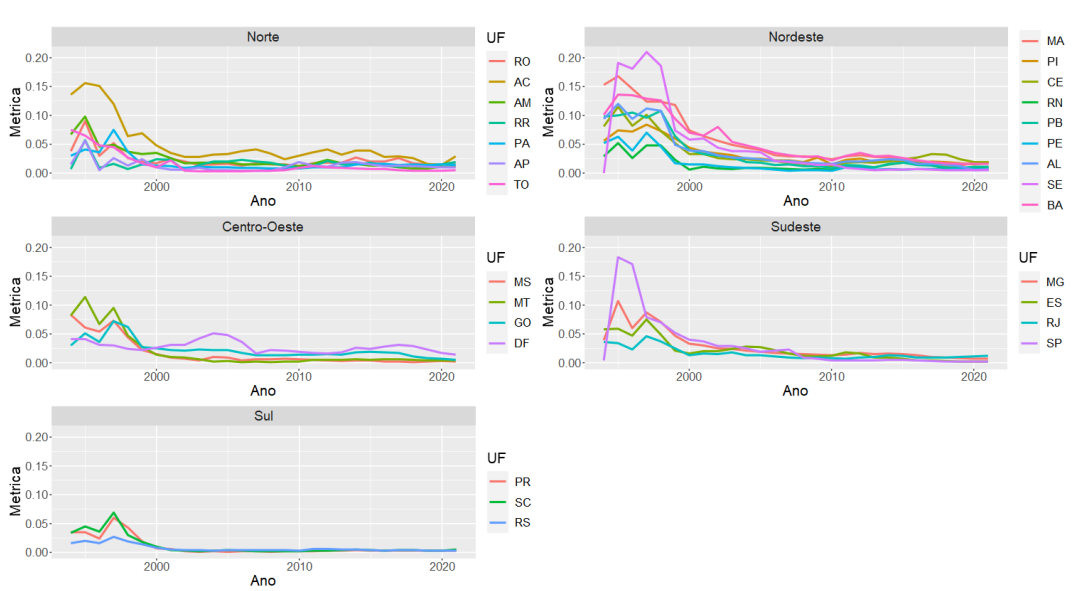
\includegraphics[width=6in]{imagens/o-que-se-tem.PNG}
     \legend{\footnotesize Legenda: Valor zero representa preenchimento de todos os campos. Quanto mais distante de zero, maior o uso das categorias “ignorado” e afins.}
    \fonte{\citeonline{completude_sinasc}}
\end{grafico}


Apesar de \citeonline{completude_sinasc} identificarem uma melhora no preenchimento das variáveis do Sinasc ao longo do tempo, sua análise não contempla a variável para idade do pai ou responsável, que não é disponibilizada através do tabulador Tabnet, apenas disponível através dos microdados. Embora a completude do sistema, de maneira geral, apresente melhorias, parece haver diferenças regionais e estaduais quanto à observação do campo idade do pai ou responsável, como veremos na próxima seção. Uma hipótese é de que possíveis diferenças na postura das Secretarias Municipais de Saúde (SMS) em relação ao preenchimento da variável podem ter afetado a relevância dada ao quesito.

A versão da DNV em uso foi atualizada em 2021 e é composta por 52 variáveis, distribuídas em oito blocos: I - IDENTIFICAÇÃO DO RECÉM-NASCIDO (seis variáveis: data, hora, sexo, raça/cor do recém-nascido, peso ao nascer, Índice de Apgar, detectada alguma anomalia congênita), II - LOCAL DA OCORRÊNCIA (sete variáveis: local da ocorrência, estabelecimento, endereço da ocorrência, CEP, bairro/distrito, município de ocorrência, UF), III - PARTURIENTE (14 variáveis: nome, cartão SUS, escolaridade (última série concluída), ocupação habitual, data nascimento, idade, naturalidade, situação conjugal, raça/cor, residência, logradouro, CEP, bairro/distrito, município, UF), IV -RESPONSÁVEL LEGAL (duas variáveis: nome, idade), V - GESTAÇÃO E PARTO (11 variáveis: histórico gestacional, data da última menstruação (DUM), número de semanas de gestação, número de consultas de pré-natal, 34 Mês de gestação em que iniciou o pré-natal, tipo de gravidez, apresentação\footenote{Com relação ao recém nascido. As opções são: 1 – Cefálica; 2 – Pélvica ou Podálica; 3 – Transversa 9 – Ignorado.}, o trabalho de parto foi induzido?, tipo de parto, cesárea ocorreu antes do trabalho de parto iniciar, nascimento assistido por), VI - ANOMALIA CONGÊNITA (uma variável de campo aberto para descrever todas as anomalias congênitas observadas no recém-nascido. ), VII - PREENCHIMENTO (seis variáveis: data do preenchimento, nome do responsável pelo preenchimento, função, tipo documento, número do documento, órgão emissor), VIII - CARTÓRIO (cinco variáveis de preenchimento exclusivo do Oficial do Registro Civil (cartórios): cartório, registro, data, município, UF)\cite{BRmanualDNV2022}.

A disponibilização do banco de dados consolidado ocorre a cada dois anos, devido aos processos de aprimoramento e qualificação dos dados de natalidade. Esses processos são realizados em três etapas junto aos estados e municípios onde há procedimentos de crítica dos dados, mediante checagem de inconsistências e possíveis duplicidades\footnote{\href{https://svs.aids.gov.br/daent/centrais-de-conteudos/dados-abertos/sinasc/}{Sistema de Informações sobre Nascidos Vivos (SINASC) - Nota Informativa.}}. Por esse motivo, nossa análise se limitará ao ano de 2022.

%

\section{Idade do pai ou responsável ao nascimento}\label{var_interesse}

Nossa variável de interesse, relativa à idade do pai, apresenta pouca documentação acerca de sua implementação e manutenção no Sinasc. A DNV passou por alguns processos de atualização. \citeonline{jorge2007quality} afirmam que no primeiro modelo de DNV estavam presentes campos para registros das seguintes informações: cartório de registro e o local de ocorrência do nascimento, informações sobre o recém-nascido (data do nascimento, sexo, peso ao nascer, índice de Apgar) e sobre a gravidez (duração da gestação, tipo de gravidez e tipo de parto), características da mãe do nascido vivo (nome, idade, grau de instrução, município de residência e filhos tidos) e nome do pai. Porém, em janeiro de 1996, já passa a circular um novo modelo de DNV no país, no qual o campo para registro do nome do pai foi retirado \cite{jorge2007quality}.

\citeonline{mello1993avaliaccao} já apontavam (quando o sistema de informação sobre nascimentos era ainda operado pelo Instituto Brasileiro de Geografia e Estatística, com base nas informações do Registro Civil) sobre comportamento atípico para a variável nome do pai, em relação às demais onde, segundo eles, “a ausência de informação, neste caso, não implica, necessariamente, falha de preenchimento, podendo, também, retratar o desejo de não identificar o pai.” \cite[p.21]{mello1993avaliaccao}. Relataram, ainda, que no estudo que realizam em cinco municípios de São Paulo, um dos municípios não possuia registro para a informação porque o único hospital da cidade\footnote{Município de Pariquera-Açu.}, à época, decidiu deliberadamente omitir o dado. Concluíram que a informação relativa ao nome do pai estava sendo pouco valorizada pelos estabelecimentos de saúde. Em trecho que exprimem sua opinião, os autores afirmam: “Essa atitude vem ao encontro de opinião dos autores que julgam ser o nome do pai uma informação de caráter jurídico e não médico, epidemiológico, ou de saúde pública e, portanto, dispensável em um documento dessa natureza.”\cite[p.21]{mello1993avaliaccao}.

Não foi possível verificar porque o campo (nome do pai) foi retirado em 1996, já no âmbito do Sinasc. Somente através do dicionário de variáveis disponível no site da Secretaria de Vigilância em Saúde e Ambiente \footnote{Fonte: \href{https://svs.aids.gov.br/daent/cgiae/sinasc/documentacao/dicionario_de_dados_SINASC_tabela_DN.pdf}{Dicionário de dados da tabela DN.}} foi possível identificar que as variáveis que registram informações sobre a paternidade do nascido vivo (a saber, nome e idade do pai) fazem parte de um conjunto de novos campos criados em 2009. 

A mudança da DNV em que é introduzida, aparentemente, pela primeira vez, o registro da idade do pai ao nascimento, foi discutida e aprovada no Comitê Técnico Assessor do SIM (Sistema de informação sobre Mortalidade) e Sinasc no período de 2007 a 2009 \cite{BRConsolidacaoSINASC2011}. O processo de implementação se deu de forma gradual, após realização de teste piloto, o novo formulário foi ajustado e impresso em 2010. O CTA decidiu por uma estratégia de não substituir abruptamente a DNV antiga pela nova versão, fazendo com que o modelo antigo e o novo circulassem simultaneamente.

Apesar da orientação de que, a partir de janeiro de 2011, fosse utilizado preferencialmente os formulários novos, naquele ano ainda houve uma proporção expressiva dos nascimentos sendo registrados no modelo antigo da DNV. Segundo relatório da Coordenação Geral de Informações e Análise Epidemiológica \cite{BRConsolidacaoSINASC2011}, a base de dados do Sinasc de 2011 é constituída de 58\% de formulários novos (com informação para idade do pai), e 42\% de formulários antigos. Por região, a participação do formulário novo variou, sendo maior no Nordeste (88\%), e menor no Sudeste (35\%). O Centro-Oeste teve, proporcionalmente, a segunda maior utilização de formulário novos (76\%), seguido pelo Norte (68\%), e pelo Sul (39\%). Devido aos campos com informações sobre a paternidade serem coletados somente a partir do novo modelo adotado em 2009, a análise terá início em 2012.

Em sua última atualização, o 8º modelo da DNV distribuído a partir de agosto de 2021, os campos para registro de informações paternas foram modificados, para se adequar a novos modelos de parentalidade e arranjos familiares\footnote{Fonte: NOTA TÉCNICA Nº 195/2021-CGIAE/DASNT/SVS/MS. Disponível em: https://dive.sc.gov.br/phocadownload/SINASC/Legisla\%C3\%A7\%C3\%A3o/NTF-n195-2021.pdf}.
O “bloco IV - Pai”, contendo o nome e idade do pai, passa a ser “Bloco IV– Responsável legal”, onde deve ser registrado o nome do(s) responsável(eis) legal(ais)\footnote{É possível registrar, inclusive, dois responsáveis legais, nesse caso, fica registrada a idade do  primeiro responsável legal inscrito.} \cite{BRmanualDNV2022}. Os campos para registro das informações paternas, desde sua implementação 2009-2010, não são de preenchimento obrigatório e não é necessário, nem suficiente, para o reconhecimento da paternidade. Ou seja, ter o nome do pai registrado na DNV não dá legitimidade legal à paternidade do nascido vivo, esse procedimento é somente realizado em cartório \cite{BRmanualDNV2011}. A não utilização dos termos “pai” e “mãe” ocorre para que seja contemplada a filiação, independentemente da identidade de gênero, como nos casos de reprodução assistida, casais transgêneros, união homoafetiva e outras situações similares. Nos campos para “Responsável legal” não têm, necessariamente, a idade do genitor do nascido vivo registrada. Porém, admite-se que o registro de nascimentos havidos por reprodução assistida ou de gestação por substituição ainda ocorram em proporção tal que não devem alterar as estimativas.

Fazendo uma avaliação da completude do preenchimento para a variável idade do pai ou responsável no Sinasc, podemos avaliar que 2012 foi o ano com menor proporção de registros ignorados. No decorrer dos anos, a completude da variável apresenta piora, chegando a mais de 60\% de dado faltante de 2018 em diante (gráfico \ref{graf:FaltanteBrasil})\footnote{Os gráficos apresentados nessa seção serão alterados para contemplar os anos de 2021 e 2022.}. Tal comportamento pode decorrer da falta de valorização destinada à variável, como ilustrado pela perspectiva de \citeonline{mello1993avaliaccao}, da percepção dessa informação como algo não associado à saúde pública ou sem valor jurídico (para a afirmação da paternidade) e, portanto, vista como não valiosa para o contexto do documento. 

\begin{grafico}
    \centering
    \caption{Percentual de dados faltantes para a idade do pai ou responsável - Brasil - 2012-2020}
    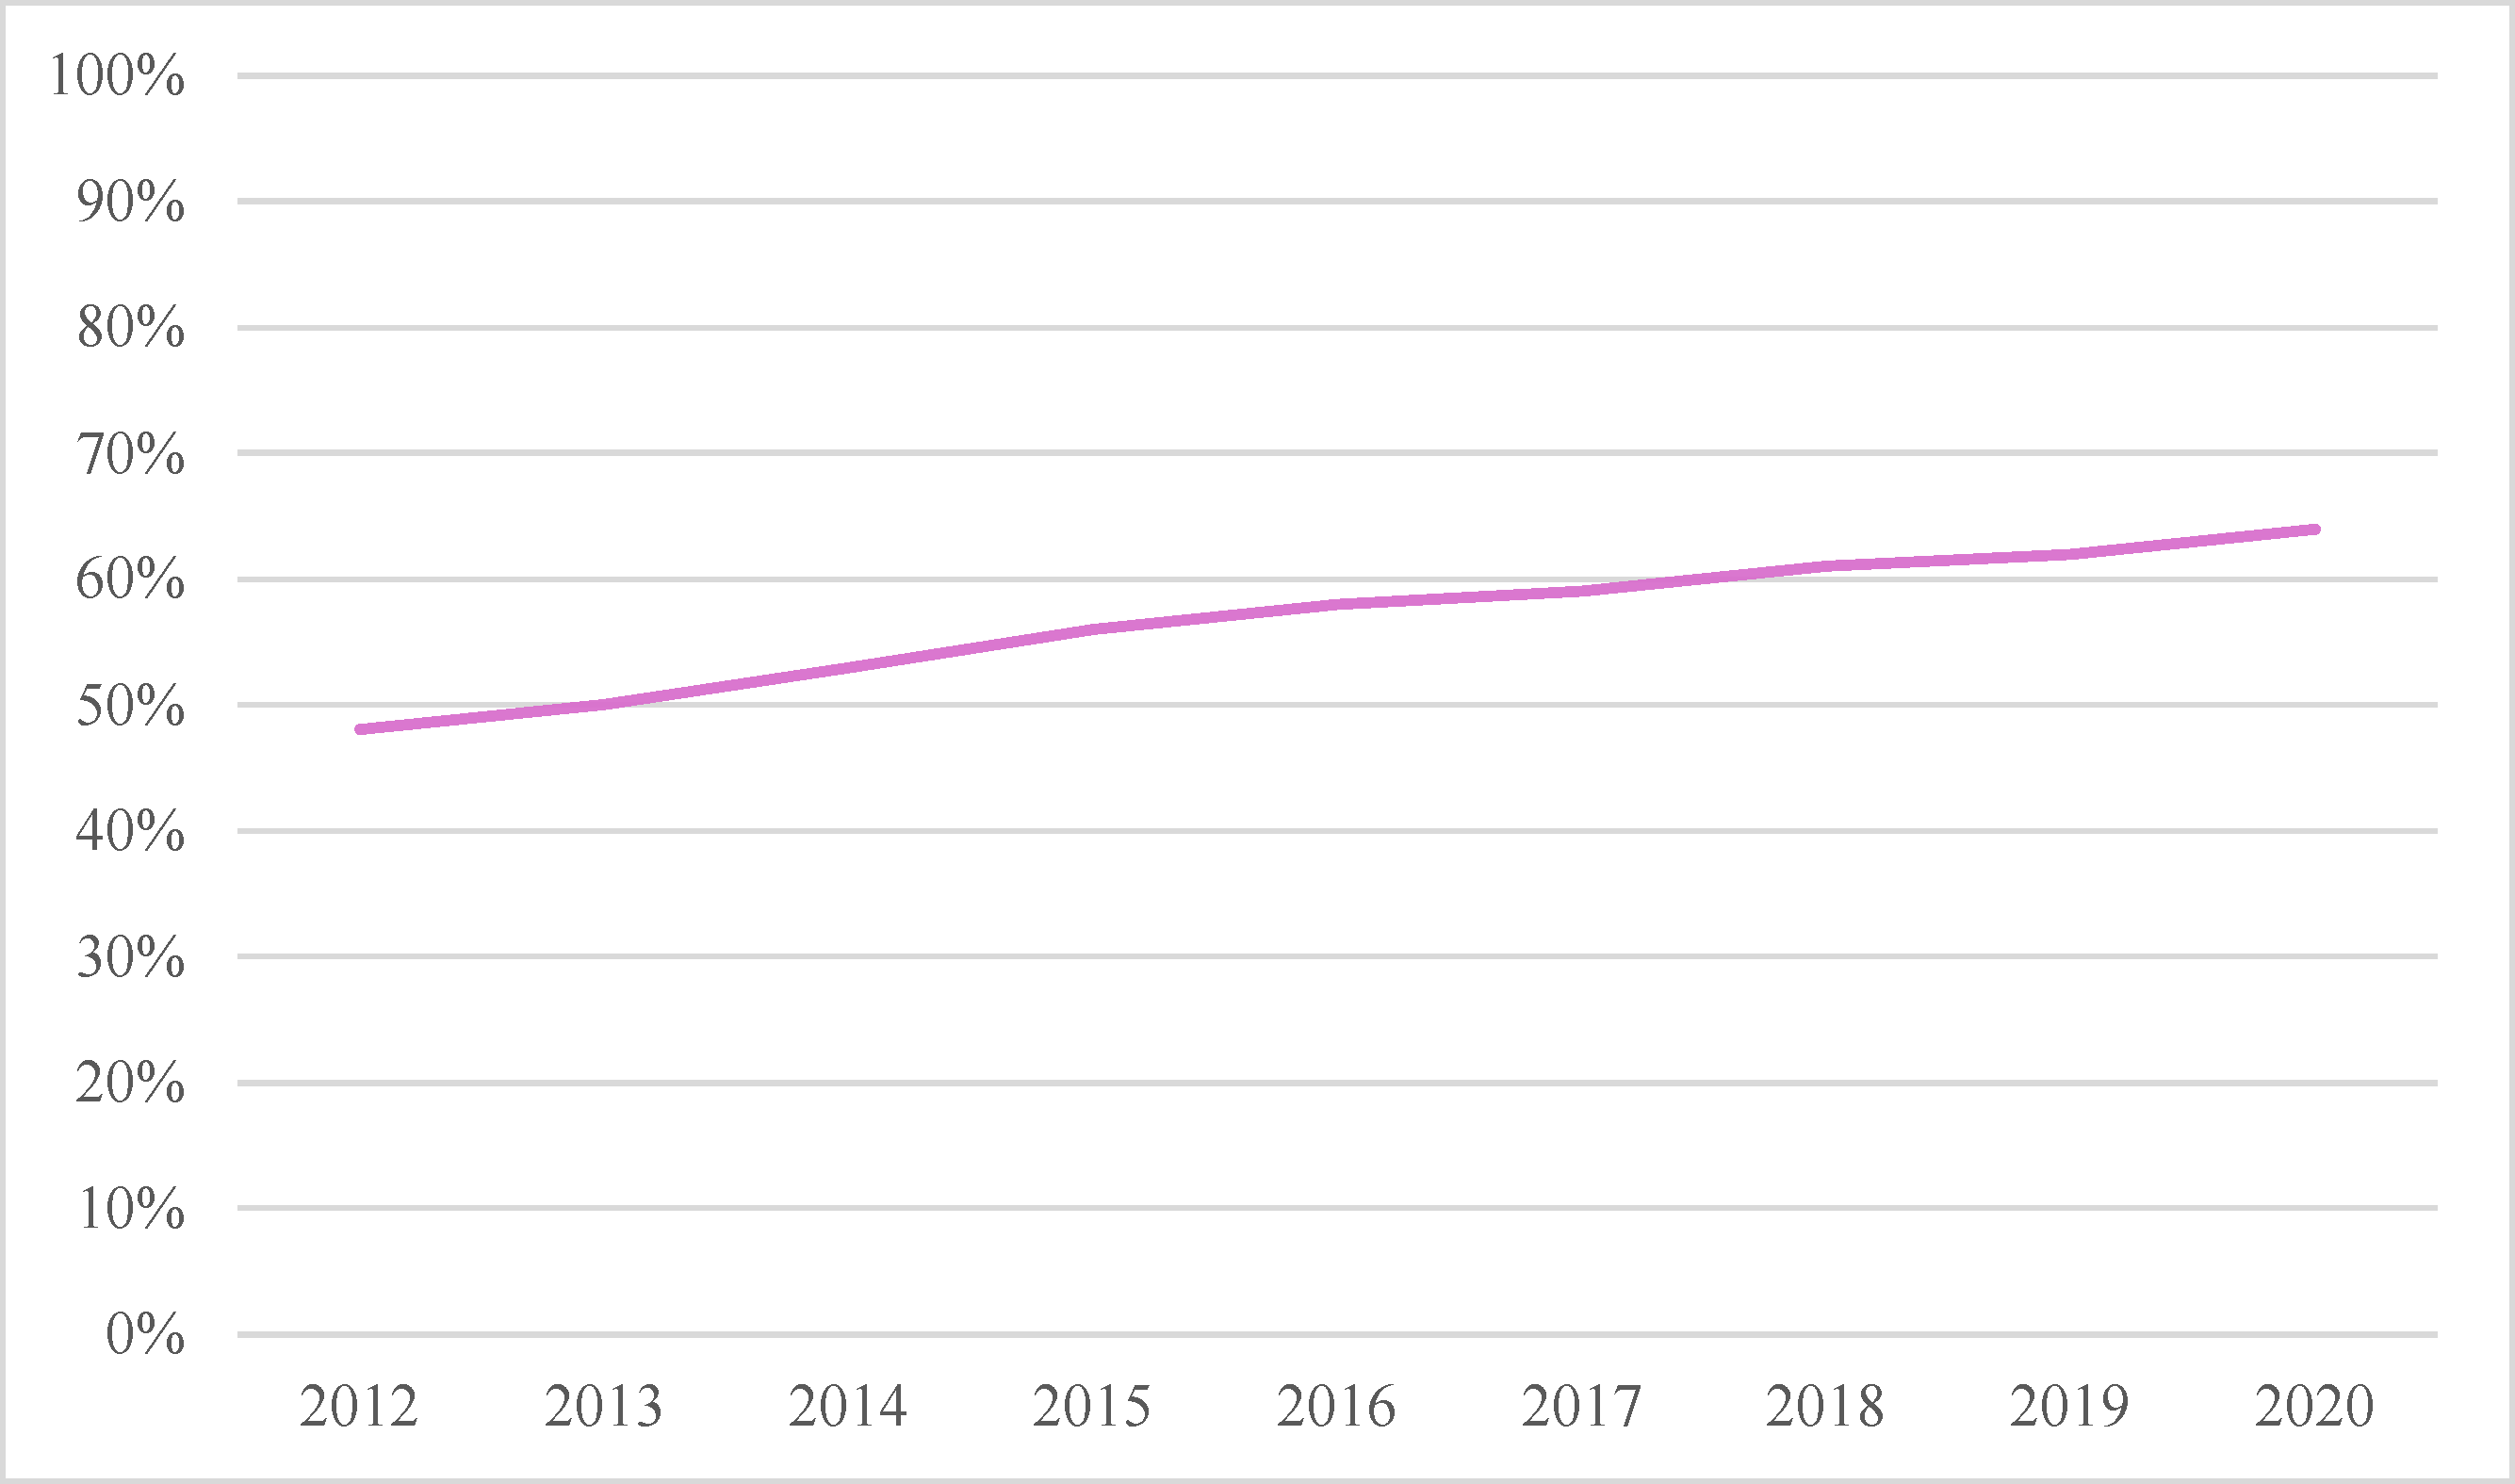
\includegraphics[width=5.0in]{imagens/Proporção de dados faltantes para idade do pai 2010-2020 nível Brasil.pdf}
    \fonte{Datasus - Sinasc}
    \label{graf:FaltanteBrasil}
\end{grafico}

A distribuição dos valores faltantes não acontece de maneira homogênea entre as regiões e UFs. Observando os gráficos \ref{graf:sudeste} ao \ref{graf:nordeste} vemos comportamentos diferentes. A região Sudeste apresenta percentuais semelhantes de valores faltantes entre as UFs, com valores concentrados entre 30\% e 40\% no início do período e entre 50\% e 60\% em 2020.

\begin{grafico}
    \centering  
    \caption{Percentual de dados faltantes para a idade do pai ou responsável - Região Sudeste - 2012-2020}
    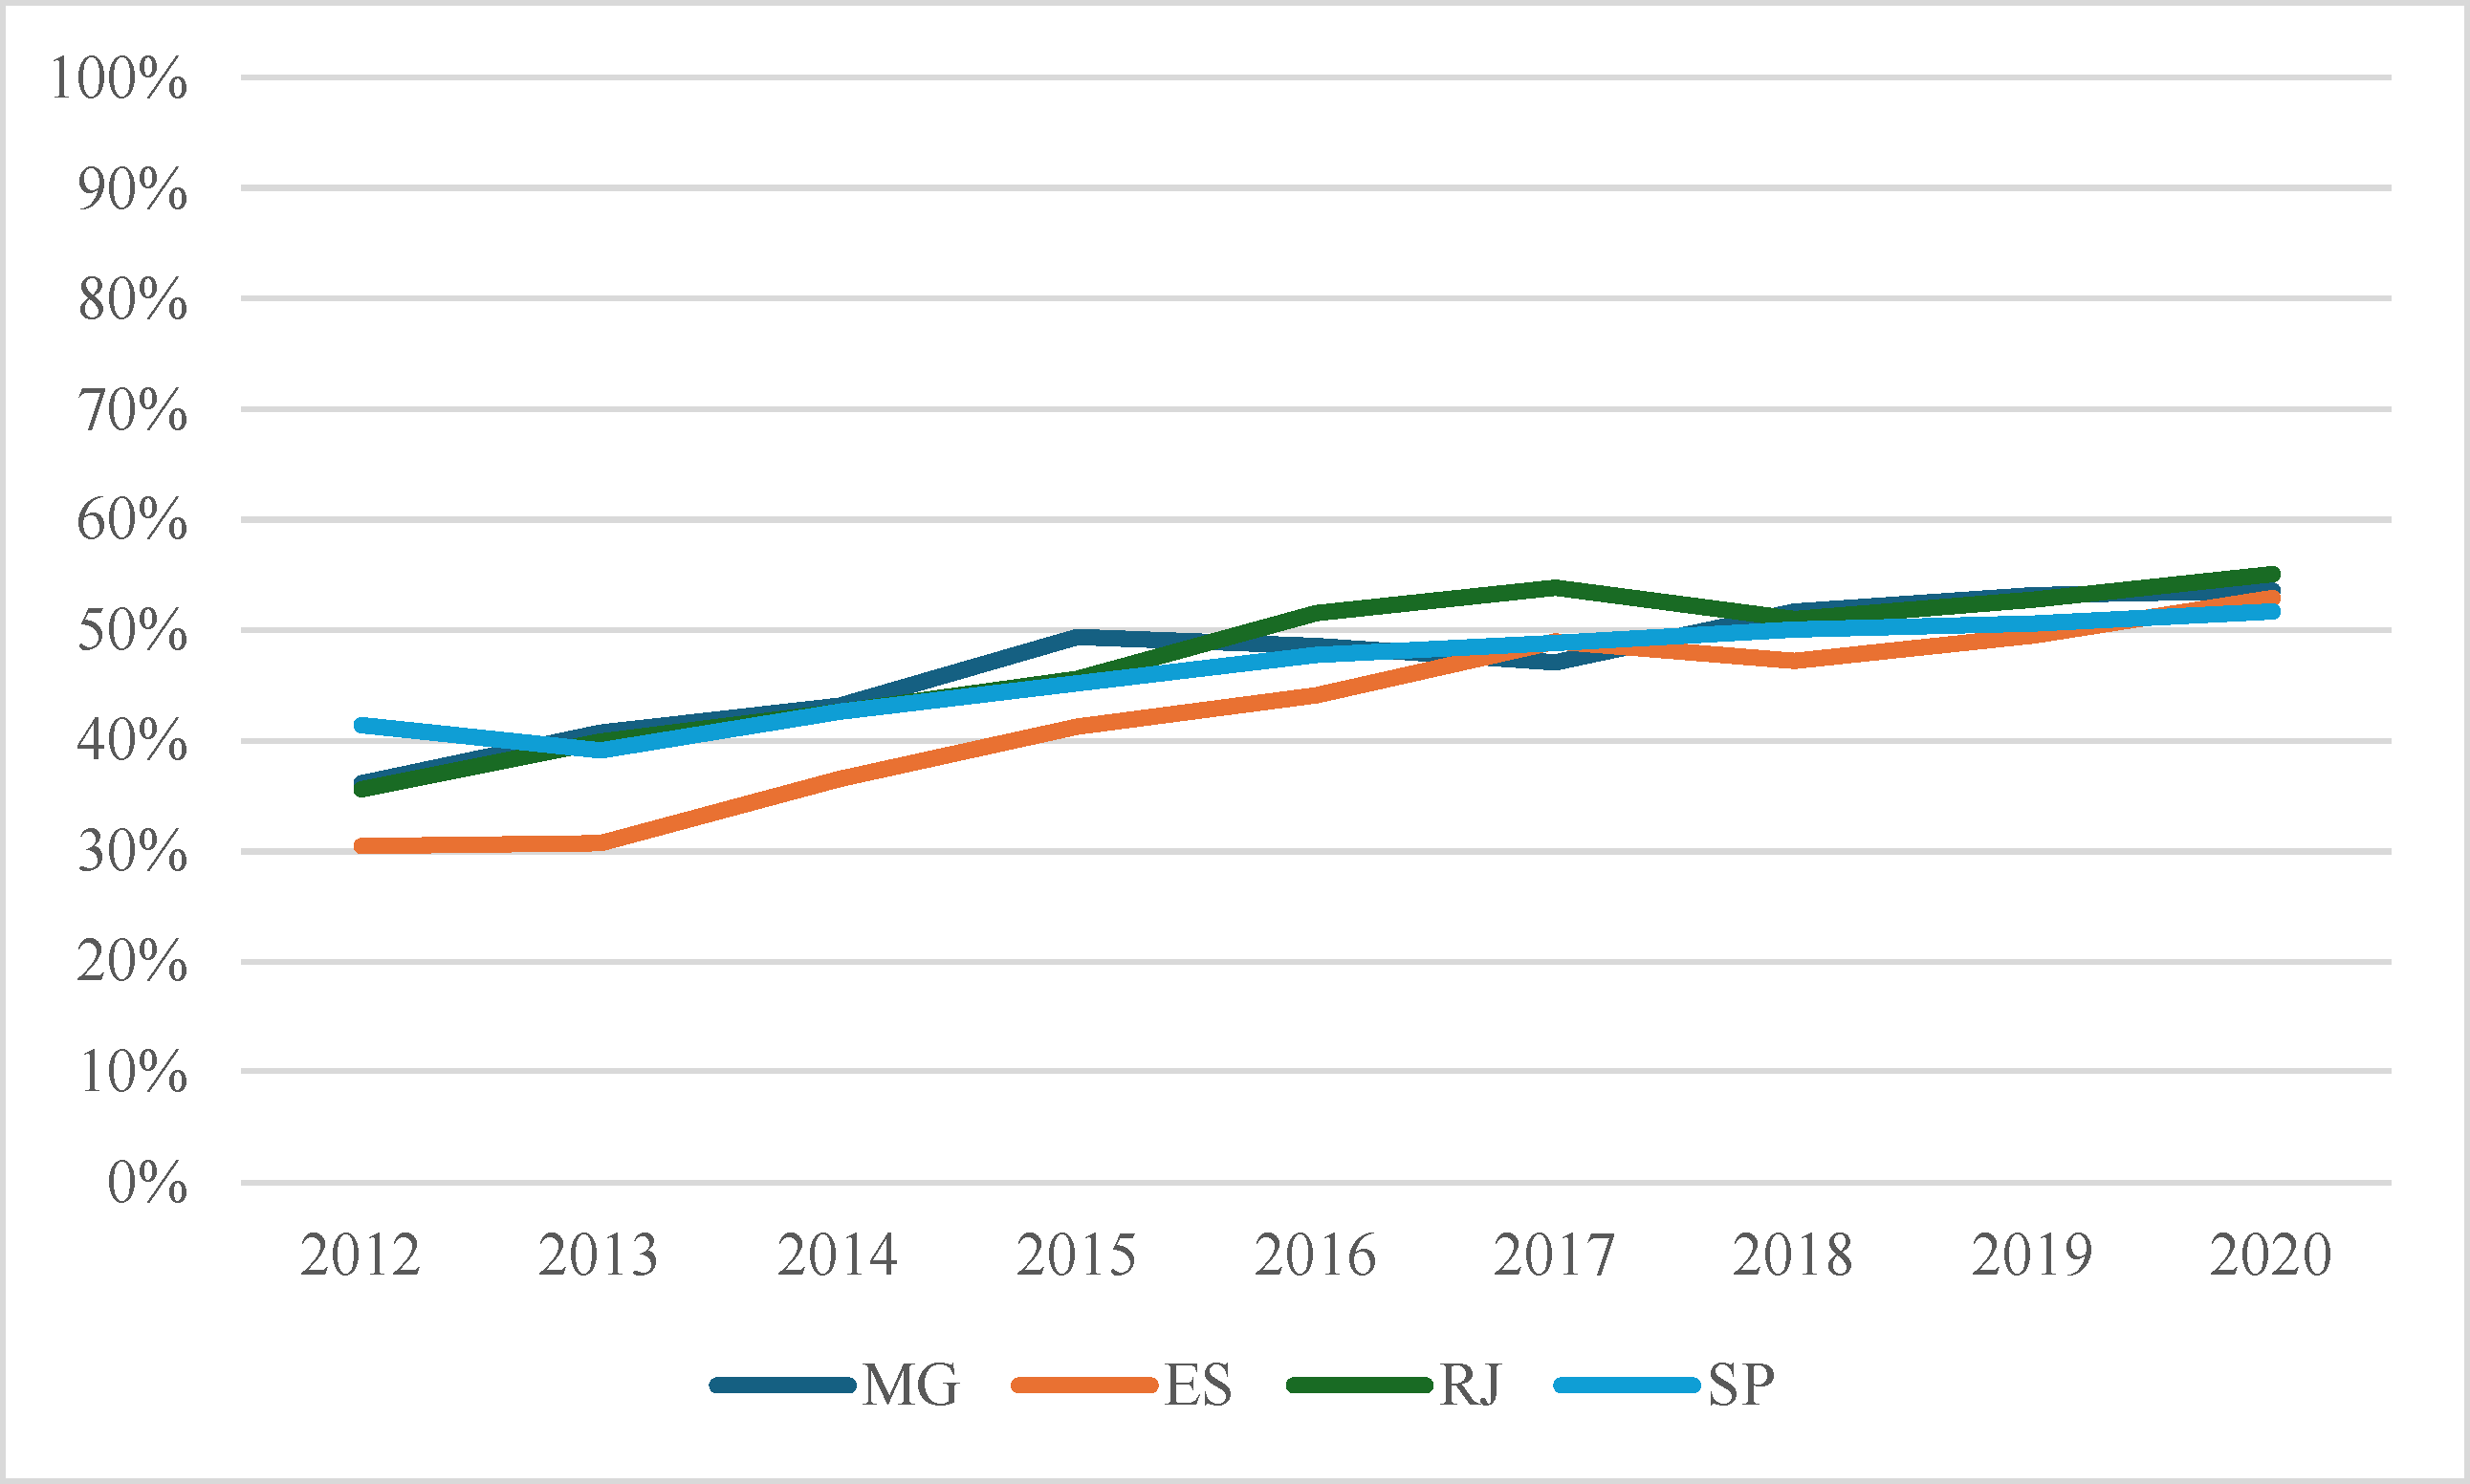
\includegraphics[width=5.0in]{imagens/faltantes-sudeste.pdf}
    \fonte{Datasus - Sinasc}
    \label{graf:sudeste}
\end{grafico}

Já os valores para o gráfico \ref{graf:sul} são mais discrepantes entre os estados, com Santa Catarina apresentando 45\% de dado faltante em 2012, enquanto Paraná o valor encontrado foi de 13\% para o mesmo ano. O Paraná foi a UF que apresentou as menores proporções de dados faltantes no período. Observa-se, porém, que o padrão de crescimento da não observação da idade do pai também ocorre no estado, alcançando o mesmo nível de dado faltante que o Rio Grande do Sul em 2020, em 33\%.

\begin{grafico}
    \centering  
    \caption{Percentual de dados faltantes para a idade do pai ou responsável - Região Sul - 2012-2020}
        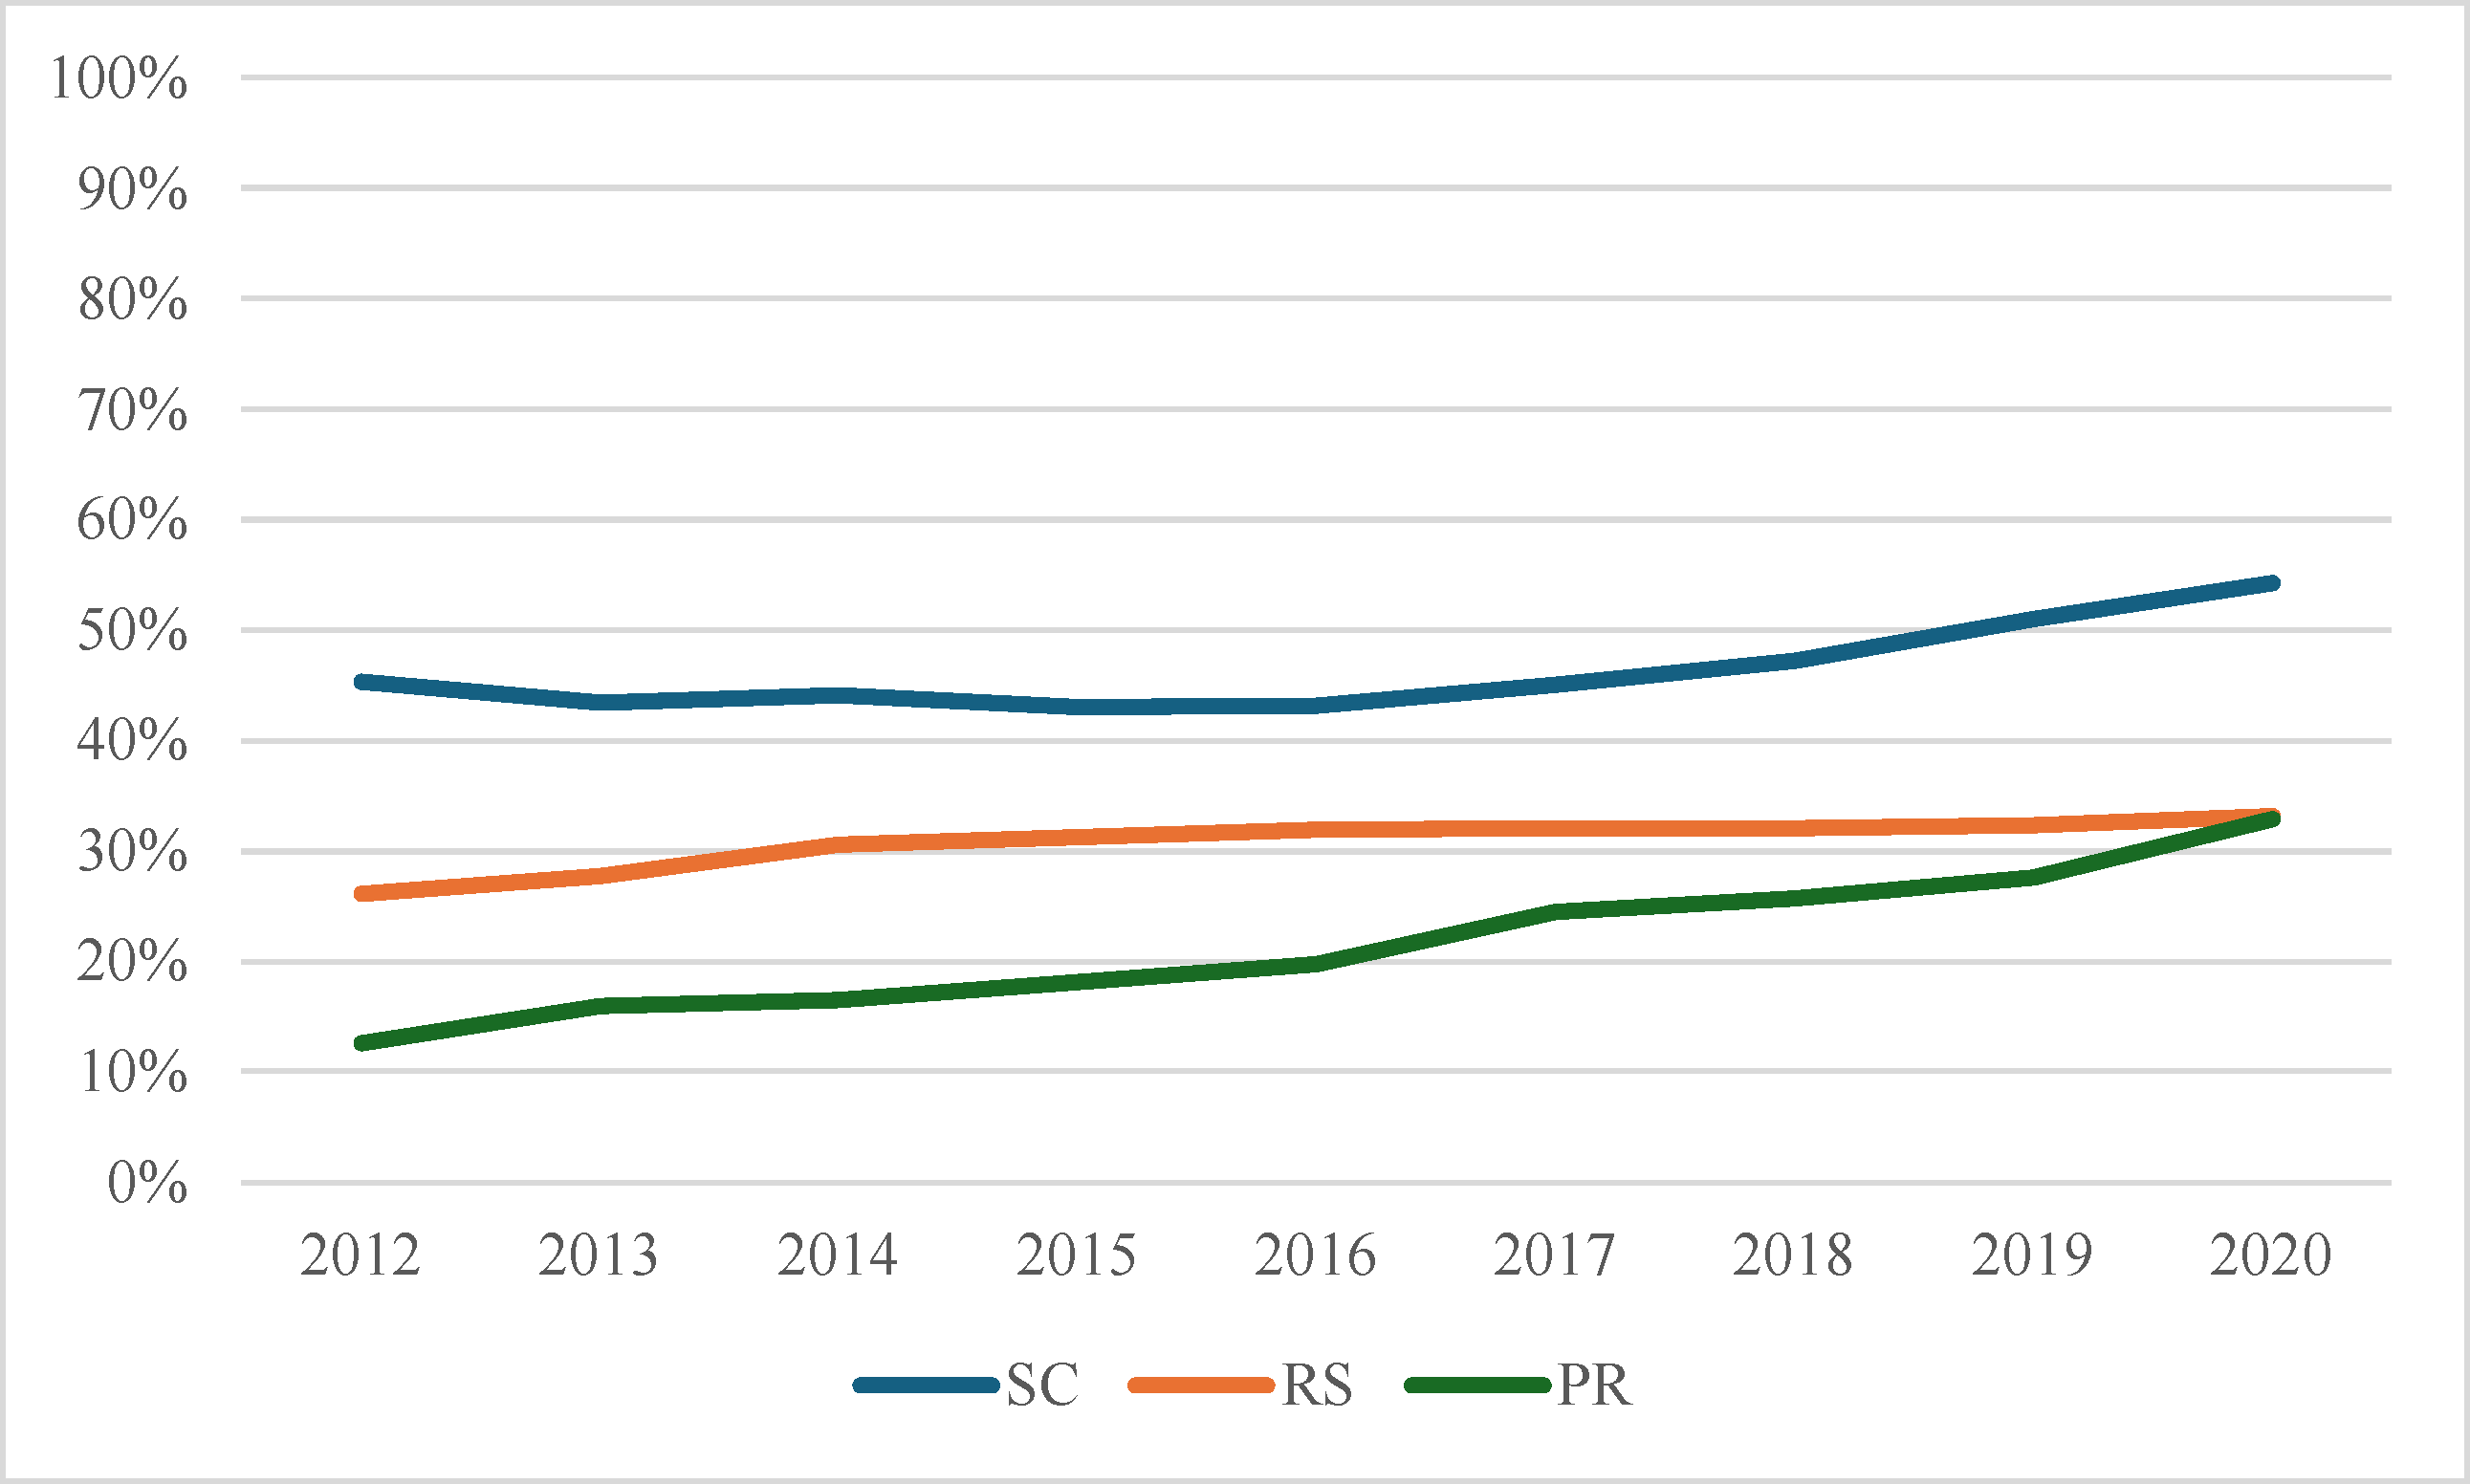
\includegraphics[width=5.0in]{imagens/faltantes-sul.pdf}
    \fonte{Datasus - Sinasc}
    \label{graf:sul}
\end{grafico}

\begin{grafico}
    \centering  
    \caption{Percentual de dados faltantes para a idade do pai ou responsável - Região Norte - 2012-2020}
           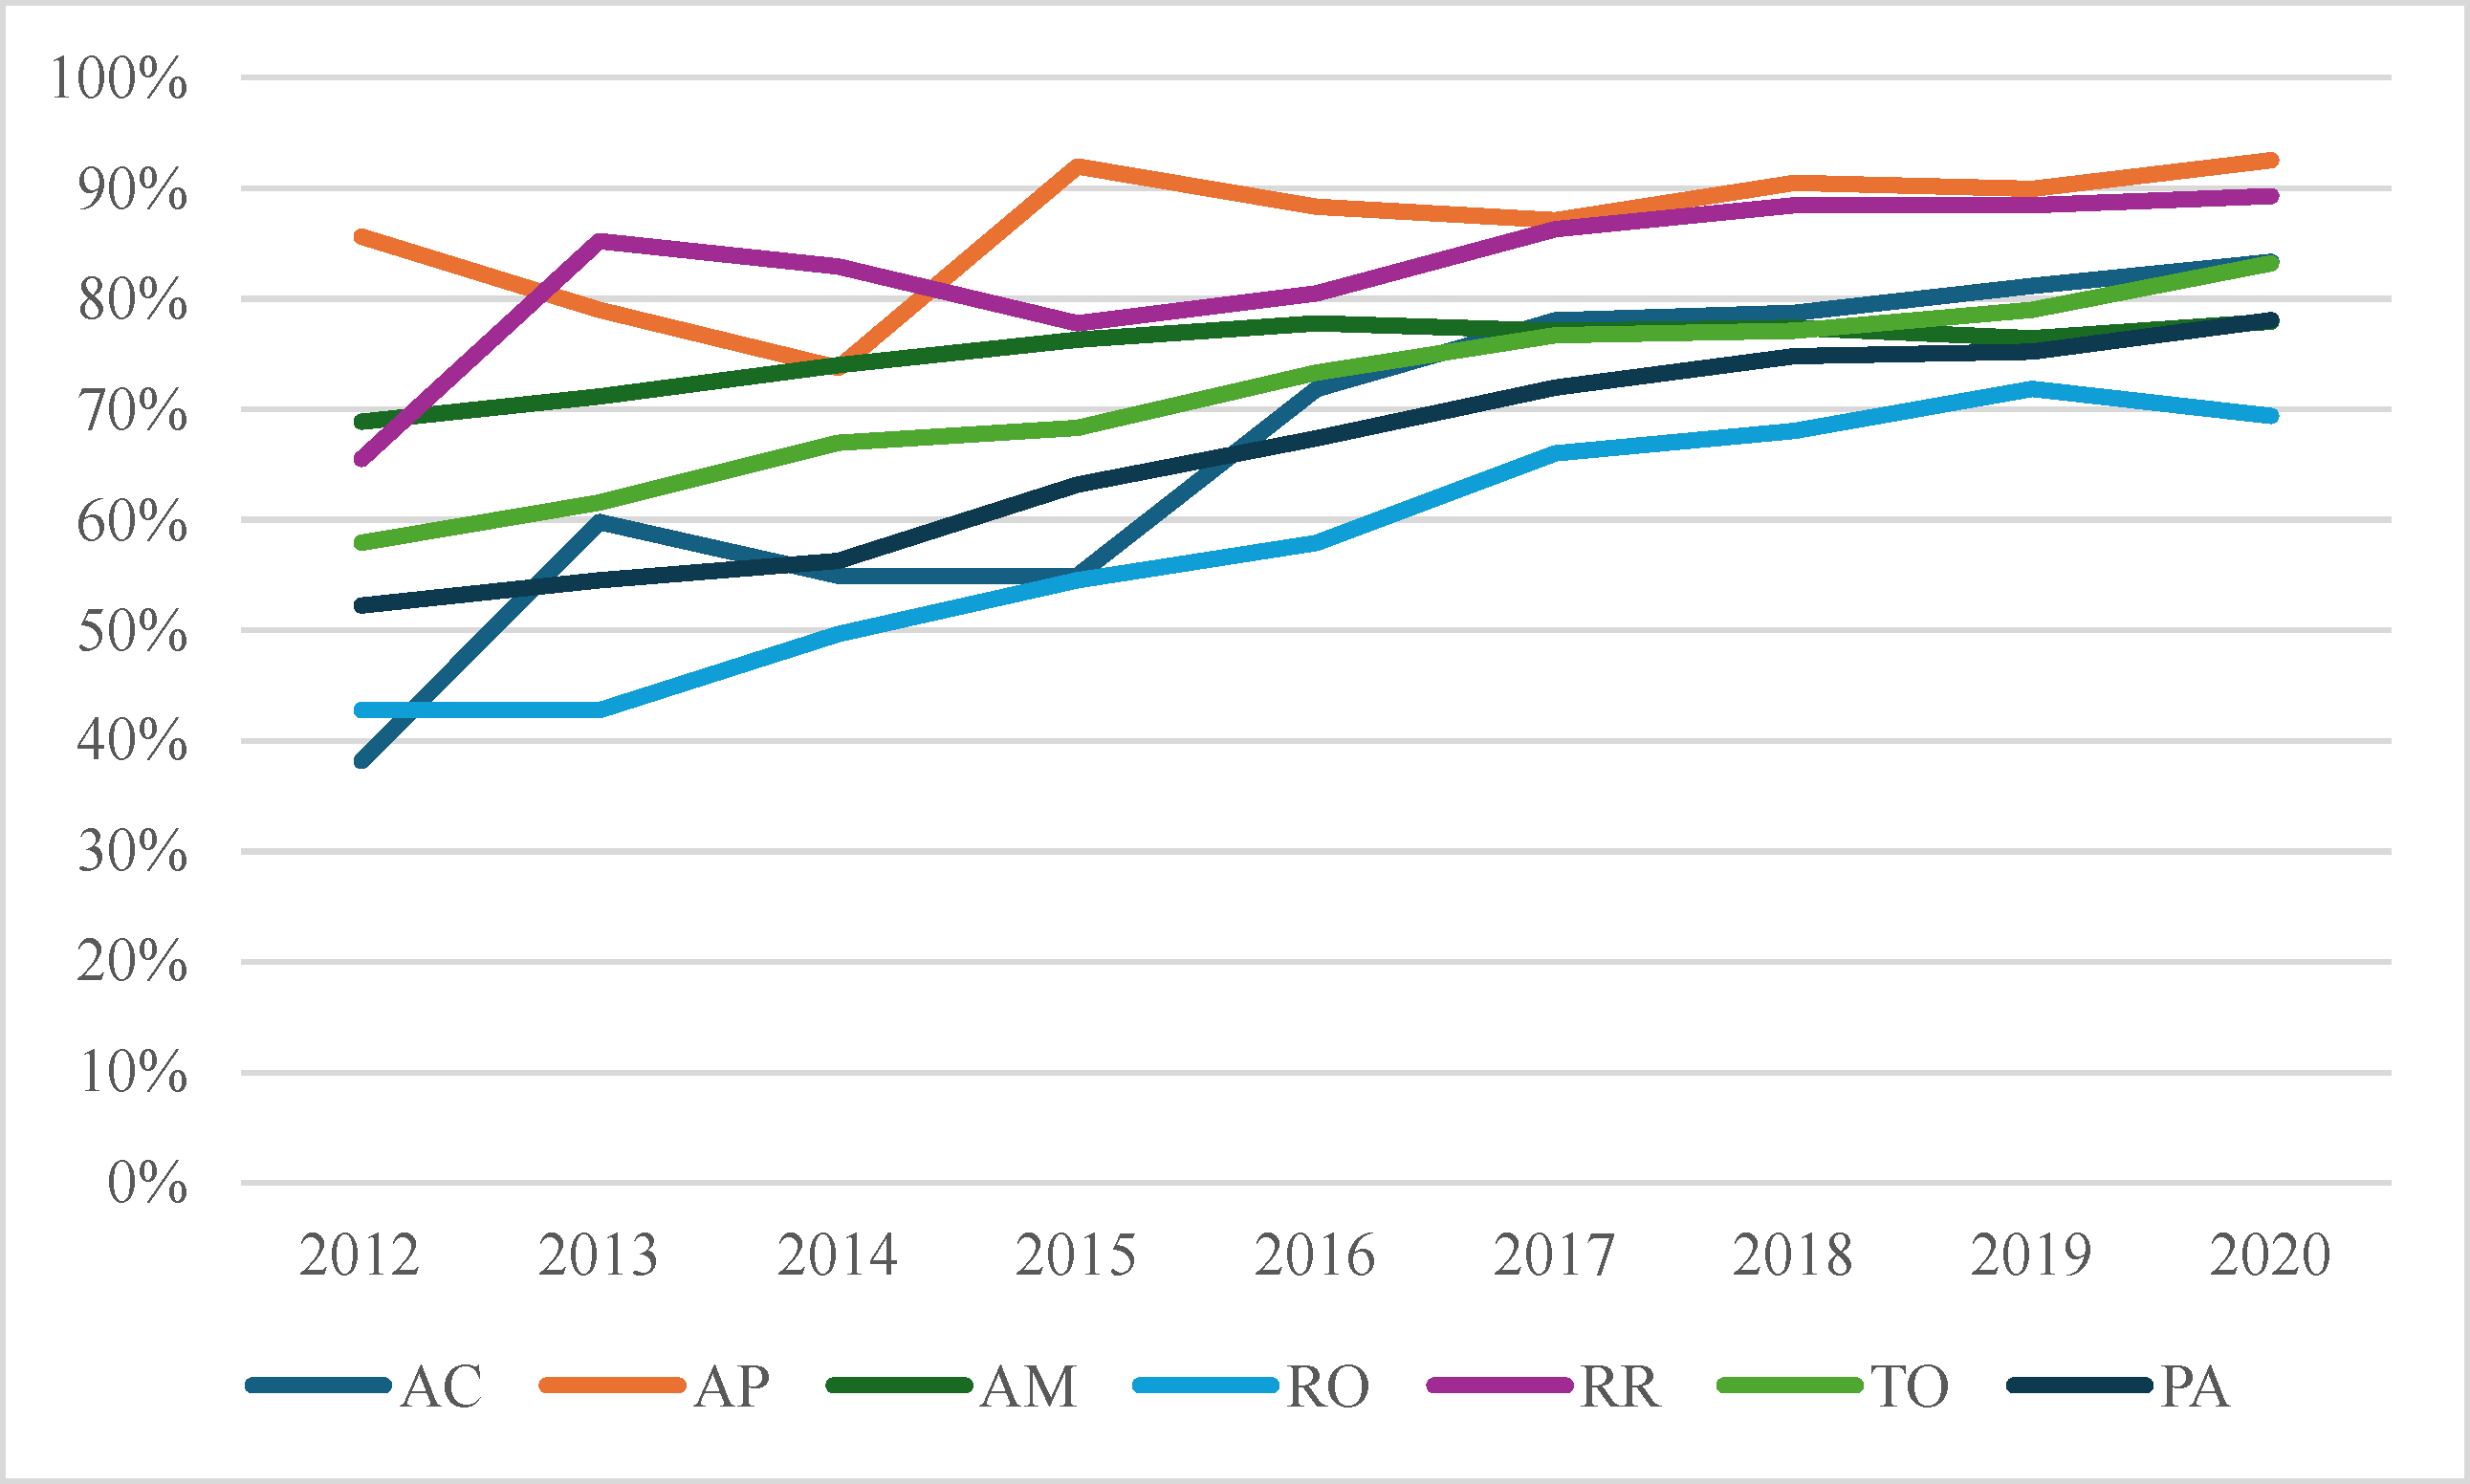
\includegraphics[width=5.0in]{imagens/faltantes-norte.pdf}
    \fonte{Datasus - Sinasc}
    \label{graf:norte}
\end{grafico}

\begin{grafico}
    \centering  
    \caption{Percentual de dados faltantes para a idade do pai ou responsável - Região Centro-Oeste - 2012-2020}
   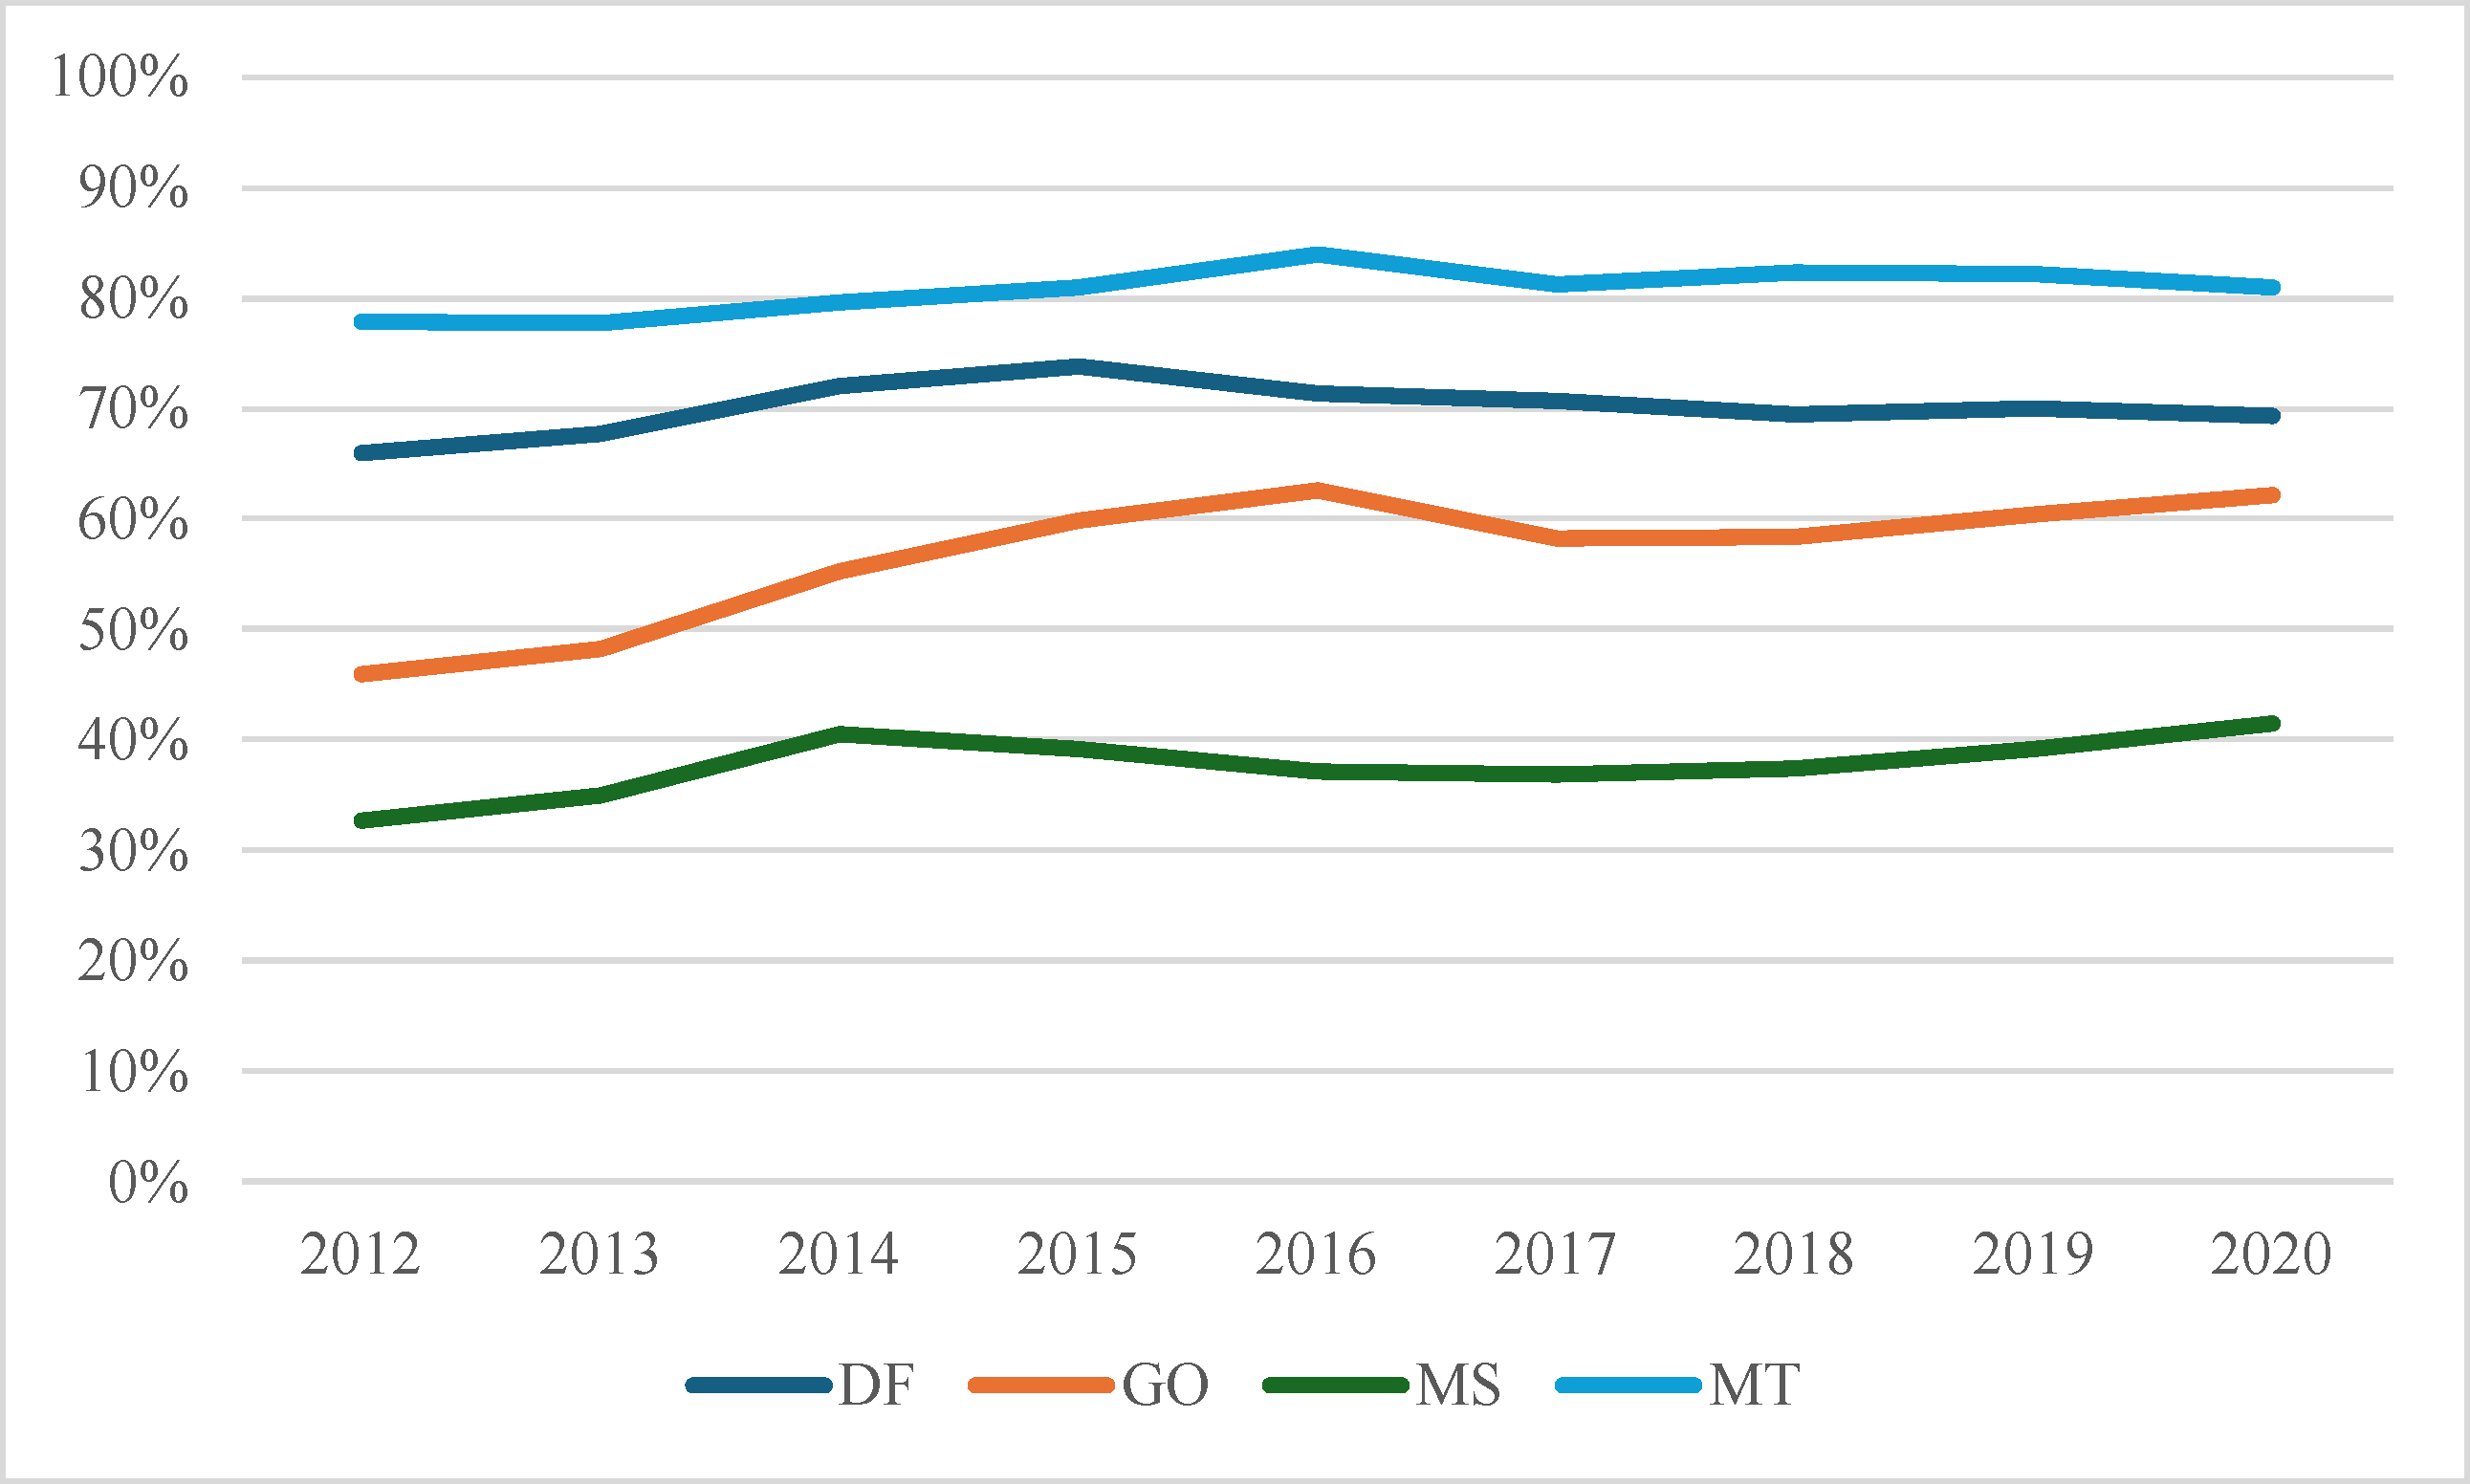
\includegraphics[width=5.0in]{imagens/faltantes-centro-oeste.pdf}
    \fonte{Datasus - Sinasc}
    \label{graf:centro-oeste}
\end{grafico}

\begin{grafico}
    \centering  
    \caption{Percentual de dados faltantes para a idade do pai ou responsável - Região Nordeste - 2012-2020}
        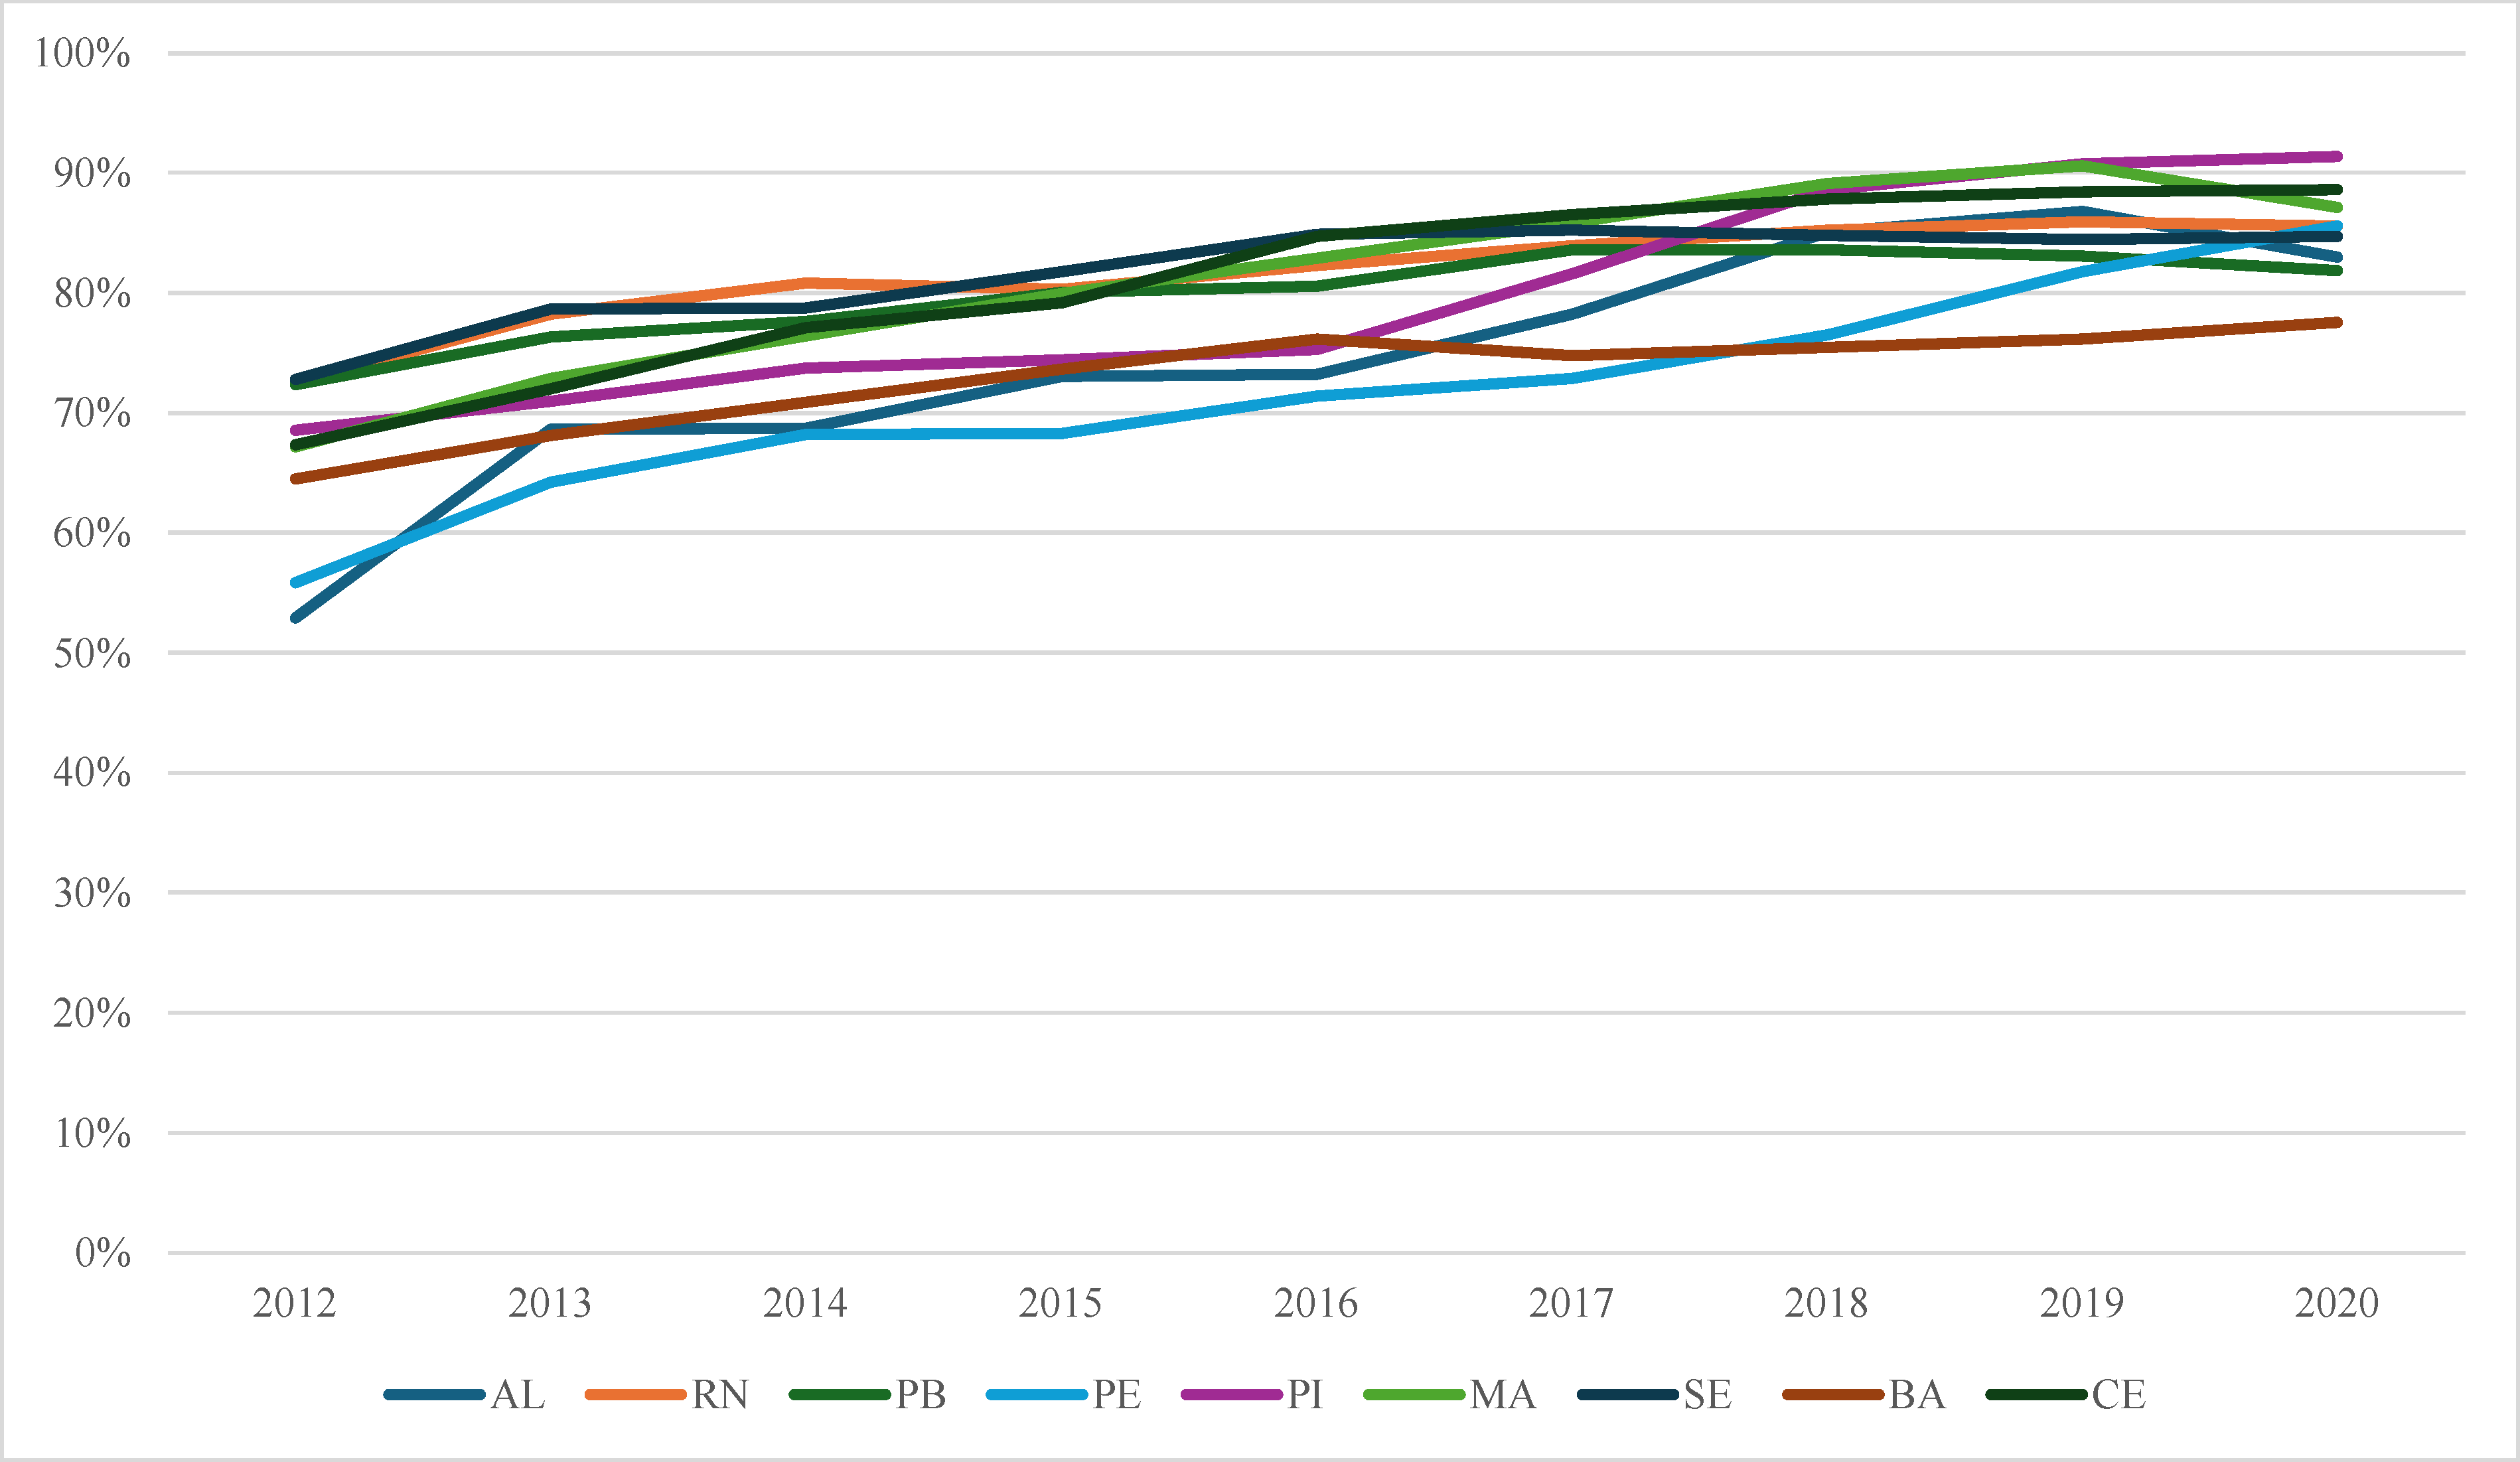
\includegraphics[width=5.0in]{imagens/faltantes-nordeste.pdf}
    \fonte{Datasus - Sinasc}
    \label{graf:nordeste}
\end{grafico}

Na região Norte (\ref{graf:norte}), a proporção de dados faltantes entre as UFs varia de forma menos suavizada através dos anos. Acre e Roraima, por exemplo, apresentam uma diferença de 22\% e 20\% (respectivamente) nos percentuais de dados faltantes de 2012 e 2013. O Amapá apresentou os piores níveis do país em 2012, 2015, 2016, 2017, 2018 e 2020. Em 2020, as UFs apresentaram 93\% de valores não observados, sendo esse o pior cenário entre as UFs no período entre 2012 e 2020.


Os dados da região Centro-Oeste demonstram certa estabilidade nos níveis diferentes de valores faltantes para as UFs. O Mato Grosso apresentou os piores níveis para todos os anos na região, mantendo uma diferença maior que 40\% até 2019 em relação ao Mato Grosso do Sul, a UF com melhores níveis da região. Em 2020 a diferença entre os estados alcança 39\%, a partir de uma suave melhora do Mato Grosso e uma leve piora do Mato Grosso do Sul.

O gráfico \ref{graf:nordeste} demonstra que o Nordeste, enquanto região, apresentou os maiores níveis de valores não observados. Nenhuma das UFs chega a alcançar um nível de pelo menos metade de preenchimento para a variável. Apresentam estabilidade em níveis altos para a proporção de valores faltantes para a idade do pai ou responsável. 





\begin{comment}

          AVALIAR AS RAZÕES PARA O CAMPO SER MARCADO COMO IGNORADO OU SER DEIXADO EM BRANCO ----
        
           FALANDO SOBRE A VARIÁVEL ESCOLARIDADE DA MÃE, MAS ACREDITO QUE O MESMO VALE PARA INFORMAÇÕES SOBRE O PAI: 
        
        A incompletude da escolaridade da mãe foi caracterizada quando o campo da variável no Sinasc apresentava-se em branco ou preenchido como “ignorado”. Todavia,
        
        O campo marcado como ignorado pode estar associado a diferentes fatores. Enquanto em “branco” pode ter relação com o não preenchimento do campo pelo profissional; “ignorado” pode ser pela indisponibilidade de tal informação.
        Nesse ponto de vista, algumas publicações referiram que uma das restrições para a melhor completude da variável foi a ausência das informações no prontuário hospitalar e, para o seu preenchimento, haveria necessidade de uma entrevista com a puérpera ou seu acompanhante, o que, muitas vezes, torna-se difícil por conta de ela não estar em condições de responder ou do seu acompanhante não
        ter conhecimento sobre sua escolaridade, sendo necessária a busca de outras fontes como o cartão da gestante \cite{silvestrin2018avaliaccao}
        %https://www.scielosp.org/pdf/csp/2018.v34n2/e00039217/pt 
\end{comment}



%
\input{cap2-base/tratamento-variável}

%
\chapter{Metodologia}\label{metodo}
%%%%%%%%%%%%%%%%% METODOLOGIA %%%%%%%%%%%%%%%%%

%\chapterprecis{Referencial teórico sobre os métodos quantitativos aplicados.}


Capítulo de descrição do referencial teórico dos métodos quantitativos aplicados. Primeiramente será explorado as teorias sobre tratamento de dados faltantes, para posterior ser debatido quais os métodos mais indicados para o tratamento do caso particular, idade do pai na base do Sinasc.  



\section{Dados faltantes \textit{(missing data)}}

Ao utilizar base de dados públicas e oficiais, provenientes de pesquisas domiciliares, como as realizadas pelos institutos nacionais de estatística, é habitual encontrar bases completas, com todos os dados preenchidos e com coluna de peso para ponderação, quando necessária. Porém, muitas vezes quando lidamos como registros administrativos ou bases de pesquisa realizada para algum projeto particular precisamos lidar, muitas vezes, com o processo de crítica e imputação de dados. O que nada mais é do que o processo de lidar com erros de mensuração ou fenômenos que por ventura prejudiquem a confiabilidade dos resultados. Deve-se perguntar se os valores observados da característica de interesse dos elementos da população contêm valores não realísticos, fruto de erros de digitações ou observações e de que forma os dados não observados podem afetar a estimativa dos fenômenos que se deseja observar.  

Lidar com dados faltantes é problema comum nas pesquisas de saúde e nas bases de registros administrativos. Alguns exemplos clássicos são: o atrito em estudos longitudinais (\textit{i.e.} quando os participantes abandonam o estudo antes do término do experimento), quando algumas unidades em uma pesquisa se recusam a responder o questionário completo ou a alguma questão específica, ou ainda quando algum item num registo administrativo deixa de ser preenchido. 

Cada processo de não resposta será criado por um mecanismo, que irá gerar no banco de dados diferentes padrões de dados faltantes. Uma ferramenta comumente utilizada para ilustrar esses padrões e mecanismos é a Matriz Indicadora de Dados Faltantes (MIDF). \citeonline{Little2002-cv} definem da seguinte forma: é suposto inicialmente um dataset retangular sem valores faltantes $(n \ X\ K )$, onde $Y = (y_{ij})$, com a i-ésima linha $y_{i} = (y_{i1},...,y_{iK})$ onde $y_{ij}$ é o valor da variável $Y_{j}$ para a unidade $i$. Com a ocorrência de valores faltantes a MIDF $M=m_{ij}$, onde $m_{ij}=1$ se $y_{ij}$ é faltante e $m_{ij}=0$ se $y_{ij}$ for observado. Enquanto o padrão do dado faltante descreve quais valores são, ou não, observados da MIDF (\ref{fig:padrao_missing}), os mecanismos dizem respeito a relação entre os dados ausentes e os demais valores na matriz. 

Os padrões mais comuns, ilustrados por \citeonline{Little2002-cv} estão presentes na figura \ref{fig:padrao_missing}. O padrão (\textit{a}) representa o caso de quando a ausência de dados se restringe a uma única variável, por exemplo, quando num experimento planejado, em que são analisados um conjunto de fatores sobre uma variável de interesse, é pressuposto que todas sejam totalmente observadas, porém, ocorre de uma variável não estar presente (pensando em ensaios agrícolas ou químicos). O padrão visto em (\textit{b}) ocorre quando um grupo de variáveis possuem valores faltantes para os mesmos itens. Esse é um padrão comum em pesquisas domiciliares, onde as variáveis relacionadas, por exemplo, a localização da casa ou quadro de moradores podem estar plenamente preenchidos, porém, ocorre a recusa do morador ou falta de coleta do morador selecionado (i.e. em pesquisas em que ocorrem três estágios de seleção). Já o padrão em (\textit{c}) é comum em estudos longitudinais aonde parte dos participantes abandonam o experimento antes do final. Em (\textit{d}) ocorre quando o padrão para a ausência de informação é espalhado por toda a matriz de dados. Enquanto a combinação em (\textit{e}) ilustra casos em que variáveis não são observadas ao mesmo tempo, representado pelo exemplo de uma junção de arquivos em que a variável $Y1$ é comum ao arquivo de $Y2$ e $Y3$.

Apesar de indicarem os melhores métodos, conhecer apenas o padrão da MIDF não é suficiente.  É necessário que o pesquisador compreenda o processo de levantamento do dado, se aproprie da literatura sobre o fenômeno que esta sendo mensurado, para poder elaborar sobre o tipo de processo que levou a perda daquela informação \cite{donders2006gentle}. Captar os aspectos relacionados a ausência do dado é crucial para definir as razões para o não preenchimento, ou seja, classificar o mecanismo associado à ausência do dado. Complementarmente, assumir mecanismos ou padrões inadequados pode levar a escolha de metodologias inadequadas para lidar com o dado faltante e a estimadores viesados, levando a conclusões errôneas \cite{ayilara2019impact}.      

\begin{figure}
    \centering
    \caption{Exemplos de padrões de dados faltantes}
    \includegraphics[scale=0.80]{imagens/padrões-missing.PNG}
    \fonte{\citeonline{Little2002-cv}}
    \label{fig:padrao_missing}
\end{figure}

A partir da matriz de dados completos $Y = (y_{ij})$ e da MIDF $M = (M_{ij})$, \citeonline{Little2002-cv} definem que os mecanismos de dados faltantes são caracterizados pela distribuição condicional de $M$ dado $Y$, ou seja, $f(M|Y,\phi)$, onde $\phi$ simboliza o parâmetro desconhecido. Assim, a partir do exposto, \cite{Little2002-cv} constroem a tipologia que considera três mecanismos para dados faltantes, são eles: 

\begin{itemize}
    \item DADO FALTANTE COMPLETAMENTE ALEATÓRIO - \textit{MCAR (Missing Completely at Random)}
\end{itemize}
  
Se a ausência do dado não depende dos valores completos $Y$, faltantes ou observados, categoriza-se o mecanismo do dado faltante como completamente aleatório, isto é, onde o modo para o qual os dados não são preenchidos, é totalmente aleatório, não relacionado a nenhum valor. Ou seja, a probabilidade do dado faltante condicionado pelos valores completos $Y$ e pelo parâmetro $\phi$ é igual para todos os valores de $Y$ e parâmetros $\phi$.

\begin{equation} \label{relacao_data}
f(M|Y, \phi)= f(M|Y, \phi) \quad   \forall \quad  Y, \phi. 
\end{equation}
    
Como explicita \citeonline{donders2006gentle}, quando o mecanismo MCAR ocorre, as observações para as quais existem valores faltantes compõe uma amostra aleatória do dado completo, ou seja, os valores observados são representativos para a população. Teoricamente, se MCAR, apesar dos valores faltantes, as idades dos pais observadas seriam suficientes para estimar a TFT brasileira. Um exemplo trazido pelo autor é de quando um tubo de ensaio com uma amostra de sangue ou um questionário de um entrevistado é perdido acidentalmente. A falta do dado não está relacionado a nenhuma característica do paciente do qual o sangue foi retirado ou à pessoa entrevistada, i.e., a probabilidade de a observação não ter sido realizada é totalmente ao acaso. Nesse comportamento, os dados observados também compõe uma amostra não viesada para os dados completos. 

Já \citeonline{Newman2014-gs} em seu trabalho define o mecanismo MCAR quando: a probabilidade de que um valor seja faltante não depende dos valores dos dados observados nem dos valores faltantes em si, $[p(dado faltante|dados completos) = p(dado faltante)]$. Não há relação entre o mecanismo da ausência de dados e as variáveis em análise. Segundo \citeonline{nunes2007metodos}, esse mecanismo impõe que a probabilidade de não-resposta seja a mesma para diversas situações, não se altera independentemente da proporção de dados faltantes.

\begin{itemize}
    \item DADO FALTANTE ALEATÓRIO - \textit{MAR (Missing at Random)}
\end{itemize}


Por outro lado, quando os valores faltantes dependem somente de componentes observados, o mecanismo presente é denominado dado faltante aleatório. Segundo \citeonline{Little2002-cv}, assume-se ${Y_{obs}}$ como as características observadas ou entradas de $Y$, e ${Y_{mis}}$ como os valores faltantes. Atribui-se que a probabilidade do valor ser faltante depende somente de valores observados, ${Y_{obs}}$ de $Y$, e não dos valores ausentes. Logo, \citeonline{Little2002-cv} formalizam:

\begin{equation} \label{mar_equ}
f(M|Y, \phi)= f(M|{Y_{obs}}, \phi) \quad   \forall \quad Y_{mis},\phi. 
\end{equation}

Considera-se o mecanismo MAR se a distribuição condicional de $M$ dado $Y$ é igual à distribuição de $M$ dado ${Y_{obs}}$ para todo ${Y_{miss}}$ para estimar o parâmetro $\phi$ \cite{rubin1976inference}. Ou seja, os valores completos para $Y$ são associados a uma ou mais características observadas ${Y_{obs}}$. Isso significa que a probabilidade de um valor não ser observado está associado a dados presentes no conjunto de dados. Trazendo para o nosso problema, \citeonline{dudel2019estimating} demonstra, por meio de imputações, simulando dados considerando dois mecanismos distintos para a ausência de dados (MCAR e MAR), que definir o mecanismo MAR para a idade do pai é mais preciso do que considerar que o dado é faltante por mecanismo completamente aleatório. Foram obtidos melhores resultados para as estimativas considerando a probabilidade de ausência da informação para a idade do pai condicional a idade da mãe. Ou seja, há probabilidade de não observar a idade do pai não é igualmente distribuída entre mães de todas as idades, mães mais jovens tem maior probabilidade de a idade do pai não ser observada \cite{dudel2019estimating}.        



\begin{comment}

\citeonline{zhang2021tutorial}:
-- ignorability.
Ignorable data are the types of missing data that can be effectively handled by modern missing data techniques such as FIML, MI and TS. Missing data needs to satisfy two conditions to become ignorable missing data: 1) the missing data are either MCAR or MAR; 2) parameters associated with the specific missing data rule are distinct from the parameters associated with the distribution of the variables in the dataset (Rubin, 1976). The second condition means that the parameters associated with the distribution of M are distinct from the parameters associated with the distribution of Y . 




\citeonline{donders2006gentle}:
Mostly, missing data are neither MCAR nor MNAR.
Instead, the probability that an observation is missing commonly depends on information for that subject that is present, i.e., reason for missingness is based on other observed
patient characteristics. This type of missing data is confusingly called missing at random (MAR), because missing data can indeed be considered random conditional on these
other patient characteristics that determined their missingness and that are available at the time of analysis.
For example, suppose we want to evaluate the predictive value
of a particular diagnostic test, and the test results are known
for all diseased subjects but unknown for a random sample
of nondiseased subjects. In this case the missing data would
be MAR: conditional on a patient characteristic that is ob-
served (here the presence or absence of the disease) missing
data are random.
Of course, it need not be that missingness
only depends on the outcome variable. But it is the simplest
situation, with one dependent or outcome variable and only
one independent or predictor variable.
ainda por \citeonline{donders2006gentle}:
Generally, when missing data are MAR,
all simple techniques for handling missing data, i.e., com-
plete and available case analyses, the indicator method
and overall mean imputation, give biased results.
However,
more sophisticated techniques like single and multiple imputations give unbiased results when missing data are
MAR.

\end{comment}



\begin{itemize}
    \item DADO FALTANTE NÃO ALEATÓRIO - \textit{MNAR (Missing Not at Random)}
\end{itemize}

O mecanismo não aleatório de geração de dados faltantes ocorre quando a probabilidade do dado não ser observado está relacionado ao dado faltante em si. Um exemplo clássico é para a variável renda, onde a uma tendência de subestimação devido à resistência de pessoas com rendas mais altas de revelarem a informação. Pensando na variável de interesse, idade do pai, seria o caso, hipoteticamente, se as idades dos pais não observadas ocorressem frequentemente a partir de determinada idade, se pais mais velhos tivessem vergonha de fazer o registro na DNV, por exemplo. 





Segundo \citeonline{enders2022applied}, na prática, os mecanismos para dados faltantes funcionam como pressupostos estatísticos para análise de dados faltantes, indicando as ferramentas mais adequadas para cada caso.




\textcolor{red}{[em construção]}



\begin{comment}



%\section{Métodos de imputação para dados faltantes}
%\section{Simulação}
%https://sci-hub.se/10.1007/s13524-011-0073-9


algoritmos de imputação  determinístico - não determinístico 

Além disso, existem algoritmos determinísticos e não-determinísticos. Os algoritmos não determinísticos podem encontrar diferentes soluções a cada execução, enquanto os
determinísticos sempre encontram a mesma solução (DE FRANÇA et al., 2006).

aleatorização -→ não deterministico... 

paramétrico

Quando é pressuposta determinada distribuição dos dados...

Modelos de imputação podem ser paramétricos ou não paramétricos...
se não paramétricos, podem ser frequentistas?

 coeficiente de correlação de Pearson é fortemente dependente da distribuição normal das variáveis, enquanto o coeficiente de correlação de Spearman é não paramétrico(Arciniegas-Alarcón e Dias, 2009).

conselhos: DOI: 10.1007/978-3-319-43742-2\13
– Always evaluate the reasons for missingness: is it MCAR/MAR/MNAR?
– What is the proportion of missing data per variable and per record?
– Multiple imputation approaches generally perform better than other methods.
– Evaluation tools must be used to tailor the imputation methods to a particular
dataset.




In order to choose the best methodological approach, several aspects must be considered. The missing mechanism is one. Another is whether to choose a parametric or a non-parametric method. The latter consideration is the same as for other statistical analyses: is it plausible that the data follow a known probability distribution, such as the normal distribution, or not.

Proportion of Missing Data and Possible Reasons
for Missingness

Besides the missing data mechanism, it is also important to consider the sample distribution in each variable, as some imputation methods assume specific data distributions, usually the normal distribution.
DOI: 10.1007/978-3-319-43742-2\_13


Abordagem paramétrica ou não paramétrica?


[porque idade do pai é faltante com mecanismo MAR?-esperada]

[Quais variáveis estão associadas a variável de interesse?]

[qual modelo de imputação é o mais adequado para a característica do conjunto de dados?]


\textbf{What should you preregister?}
\begin{itemize}
    \item Theory about why your data are missing at random/completely at random/not at random
    \item The method you plan to use to identify missingness (see Step 2)
    \item The auxiliary variables you will test
    \item The effect size or decision rule you plan to apply to determine whether a
    variable should be included as an auxiliary variable in multiple imputation
    or FIML
    \item The multiple imputation model you have chosen (with the predictor matrix
    - both key predictors and auxiliary variables - where appropriate)
    \item An explanation of how the multiple imputation model is congruent with the
    analysis model
\end{itemize}


\section{Definição do modelo proposto}


    The importance of congeniality
■ The imputation model and the analytic model must match.
■ As a general rule, whatever is included in the analytic model needs
to be included in the imputation model (e.g., interaction terms;
random intercepts, random slopes, and contextual effects in
multilevel models)



Quando É Adequado Usar Imputação (slide 2019 - Pedro Luis do Nascimento Silva e Andrea Diniz da Silva- aula 10) 

• Quando os mecanismos de geração de erros são corretamente
identificados;
• Quando informação auxiliar com bom poder preditivo está
disponível para todas as unidades amostradas, levando a
imputações que são próximas dos valores verdadeiros.
• Quando os padrões de não resposta podem ser estabelecidos
como:
o Missing Completely At Random (MCAR);
o Missing At Random (MAR).
• Pode ser difícil ou impossível imputar quando a não resposta é:
o Not Missing At Random (NMAR).
\end{comment}





%
%\include{cap4}
%
%%%%%%%%%%%%%%%%%% DESENVOLVIMENTO %%%%%%%%%%%%%%%%%
\chapter{DESENVOLVIMENTO} % CAIXA ALTA

\section{Análise exploratória dos dados}

\textcolor{blue}{mOSTRAR OS DADOS DE IDADE DO PAI AO LONGO DO TEMPO POR REGIÃO}



\begin{comment}
    ■ R packages: mi, mice, and Amelia packages include features for
model checking with core functions for imputing missing values
(van Buuren & Groothuis-Oudshoorn, 2011; Honaker et al., 2011;

Su et al., 2011). VIM and miP packages visualise imputed data
(Brix, 2012; Templ et al., 2015). These packages function to
graphically compare distribution of observed and imputed data, by
offering scatterplots for plotting observed and imputed data against
another variable. The mi package has tools to produce residual
plots to check imputation models when imputing data using MICE.
Amelia software has a diagnostic feature called overimputation to
produce cross-validation plots of mean imputed values against
observed value with 90% confidence intervals (Honaker et al.,
2011).
\end{comment}


\begin{comment}
Guia --- Missing Data and Multiple Imputation Decision Tree (1):

1. Examine patterns of missingness - for entire scales, items within scales,
patterns of missing data points, groups of people
○ Univariate descriptive statistics
■ Check for any illogical values that could be missing data codes
■ Consider implications of different data codes (e.g., missing data for
“I prefer not to answer”, “not applicable”, or because someone
didn’t provide an answer each have different implications)

○ Multivariate descriptive statistics
■ Look for outliers and try to determine whether the data are “real”
responses or can be considered skip patterns (e.g., careless
responders or straight-line responders; King et al. 2018)
■ Look for missingness at many variables simultaneously to identify
missing data patterns. For example, people might be missing all of
the cognitive tasks but none of the survey data (some example
visualizations)

2. Evaluate how much missingness you have on each variable of interest
Remember to pay attention to the percent of both item-missing data (i.e.,
skipped questions on a survey) and attrition-missing data (i.e., people that
were missing data for the entire wave - sometimes indicated by skip codes
within datasets).

3. Choose a decision rule for determining whether missingness is related to other variables in your dataset

■ This decision rule would ideally be preregistered!
■ In large datasets, p values may not be a reliable method to determine
which variables meaningfully predict missingness patterns (i.e., there may
be statistically significant differences at p < .05 because analyses are
highly powered, but these differences may not be practically or
meaningfully important).
■ Effect sizes are a perfectly valid way to determine whether something is
related to the missingness.
● How big of an effect size is big enough to matter? It depends, of
course, on what the outcome is you’re interested in. (Again, this is
where preregistration comes in handy.) Pick an effect size that is
the smallest relevant effect (Sullivan & Feinn, 2012).
● If you are struggling with what a “smallest relevant effect” might be,
some suggest a general rule of r > 0.4 correlation as a threshold for
inclusion (e.g., Collins et al., 2001; Enders, 2010) as this value
seems to find a good balance between model parsimony and
increased statistical power. (Note: you may have a “smallest
relevant effect” that is r < 0.4 - that’s okay, but make sure you
document and justify why you expect this to be the case) (UCLA
Statistical Consulting Group).

4. Check whether any auxiliary variables are related to your missingness

Auxiliary variables are variables in your data set that are not of particular
interest to your analysis, but that are either correlated with a missing
variable(s) or are believed to be associated with missingness. Auxiliary

variables will be added to the imputation model to increase power and/or
to help make the assumption of MAR more plausible, because including
these variables has been found to improve the quality of imputed values
generated from multiple imputation. This is especially important when
imputing a dependent variable and/or when you have variables with a high
proportion of missing information (Johnson & Young, 2011; Young &
Johnson, 2010; Enders, 2010).
○ You should still check for potential auxiliary variables even if your data are
MCAR or MNAR!
■ With MCAR data, just double check to make sure that there is
nothing else predicting patterns of missingness.
■ With MNAR data, your sample will be biased no matter what.
However, you can lessen any additional bias and increase your
power by using MI and including auxiliary variables that may
explain other missingness patterns.

■ Test auxiliary variables for inclusion
1) Create a new dummy variable that represents whether your key
variable is missing (missdummy=1) or not missing (missdummy=0).
2) Then predict it with auxiliary variables you think are likely to be
related to missingness (e.g., t-tests for continuous auxiliary
variables, chi-square for binary auxiliary variables, anova for
categorical auxiliary variables). For example, in many longitudinal
academic datasets, variables like parent education, mobility,
income to needs ratio, and disability status are often related to
higher dropout (attrition) in longitudinal studies.
3) Repeat this for any key variables you plan to include in the analysis
(predictors; outcomes).

■ Note: Assume that any statistical MCAR tests are actually tests for
whether your data can be listwise deleted (van Ginkel et al., 2020); also,
see FAQ
\end{comment}




\begin{comment}
        \href{exemplo1}{https://hdsr.mitpress.mit.edu/pub/4tx7h11w/release/2}
    \href{exmplo2}{https://www.researchgate.net/publication/358529185_A_reinforcement_learning-based_approach_for_imputing_missing_data}
    \begin{algorithm}
    \caption{nome do método utilizado para a simulação }\label{alg:cap}
    \begin{algorithmic}
    \Require $n \geq 0$
    \Ensure $y = x^n$
    \State $y \gets 1$
    \State $X \gets x$
    \State $N \gets n$
    \While{$N \neq 0$}
    \If{$N$ is even}
        \State $X \gets X \times X$
        \State $N \gets \frac{N}{2}$  \Comment{This is a comment}
    \ElsIf{$N$ is odd}
        \State $y \gets y \times X$
        \State $N \gets N - 1$
    \EndIf
    \EndWhile
    \end{algorithmic}
    \end{algorithm}
\end{comment}


%
%%%%%%%%%%%%%%%%%% RESULTADOS %%%%%%%%%%%%%%%%%
\chapter[RESULTADOS] {ANÁLISE DOS RESULTADOS} \label{resultados}

\begin{comment}
       \subsection{Exemplo de Tabela}
    
    \begin{table}[h]
    \centering
    \caption{Título da Tabela} \label{rotulo}
    \begin{tabular}{l|r}
    \hline 
    Col1 & Col2 \\\hline
    $x_i$ & 555  \\ \hline
    \end{tabular}
    \end{table}
    
    \subsection{Exemplo de quadro}
    
    \begin{table}[htbp]
    \center
    \caption{Título da Tabela} \label{rotulo2}
    \begin{tabular}{l|r}
    \hline 
    Col1 & Col2 \\\hline
    $x_i$ & 555  \\ \hline
    \end{tabular}
    
    \end{table}
    
    
    
    
    \begin{quadro}[htbp]
    \caption{\label{quadro_exemplo}Exemplo de quadro}
    \begin{tabular}{|c|c|c|c|}
    	\hline
    	\textbf{Pessoa} & \textbf{Idade} & \textbf{Peso} & \textbf{Altura} \\ \hline
    	Marcos & 26    & 68   & 178    \\ \hline
    	Ivone  & 22    & 57   & 162    \\ \hline
    	...    & ...   & ...  & ...    \\ \hline
    	Sueli  & 40    & 65   & 153    \\ \hline
    \end{tabular}
    \fonte{Autor.}
    \end{quadro}
 
\end{comment}

% 
%%%%%%%%%%%%%%%%%% CONCLUSÃO %%%%%%%%%%%%%%%%%
\chapter[CONCLUSÃO]{CONSIDERAÇÕES FINAIS} \label{conclusao}

\chapterprecis{Comentários finais e trabalhos futuros.}

\index{sinopse de capítulo}
%
\bookmarksetup{startatroot}% 
%
\postextual
%
\bibliography{ref}
%
 
%
% ----------------------------------------------------------
% Glossário
% ----------------------------------------------------------
%Capítulo excluído
% Consulte o manual da classe abntex2 para orientações sobre o glossário.
%
%\glossary
% ---
%\begin{apendicesenv}
%%
%\partapendices

%%%%%%%%%%%%%%%%% EDITAR APENDICES %%%%%%%%%%%%%%%%%
%% ----------------------------------------------------------
%\chapter{Capitulo}
%% ----------------------------------------------------------
%\chapter{Caplitulo 2}
%% ----------------------------------------------------------
%\end{apendicesenv}
%% 
%\begin{anexosenv}
%%
%\partanexos

%%%%%%%%%%%%%%%%% EDITAR ANEXOS %%%%%%%%%%%%%%%%%
%\chapter{Capitulo}
%% ---
%\chapter{Capitulo}
%%
%\chapter{Capitulo}
%% 
%\end{anexosenv}

%---------------------------------------------------------------------
%---------------------------------------------------------------------
\printindex
%
\end{document}